\documentclass[12pt,examcopy]{uathesis}
\usepackage{graphicx}
\usepackage{algorithm}
% \usepackage{subcaption}
\usepackage[dvipsnames]{xcolor}
\usepackage{pgfplots}
% \usepackage{algorithmic}
\usepackage{algpseudocode}
\usepackage{amssymb}
\usepackage{moreverb}
\usepackage{booktabs}
\usepackage{amsmath}
\usepackage{dsfont}
\usepackage{adjustbox}
\usepackage{tikz}
\usetikzlibrary{shapes,arrows}
\usepackage{csquotes}
\usepackage{url}
\usepackage{rotating}
% \usepackage{subcaption}


\newtheorem{definition}{Definition}

% some settings to fill pages more densely
\renewcommand\floatpagefraction{.9}
\renewcommand\topfraction{.9}
\renewcommand\bottomfraction{.9}
\renewcommand\textfraction{.1}
\setcounter{totalnumber}{50}
\setcounter{topnumber}{50}
\setcounter{bottomnumber}{50}

% \pgfplotsset{compat=1.15}

\begin{document}
\title{Concept Drift in Medical Referrals Triage}
\author{Hamish Huggard}
\department{Computer Science}
\supervisor{Yun Sing Koh}{Gillian Dobbie}
\maketitle

\frontmatter
\begin{abstract}
In many machine learning applications, the relationship being modelled may change over time, a phenomenon called concept drift. Most existing approaches to concept drift have assumed an artificially narrow specification of the problem. In this thesis we explore some new approaches to concept drift which introduce several new ``tricks" which help bridge the gap between academic concept drift detection and real data science applications. As a motivating example for our investigation, we consider a medical clinic where a decision support system is helping clinicians triage patients referred by GPs. As the triage decision making process evolves, the decision support system should be able to detect that its model has become outdated, and signal to a data scientist that it requires retraining.

We first introduce the Multiple Drift Detector framework, in which a detector for several different types of concept drift is constructed out of a single ``narrow" drift detector. This allows for a more complete and interpretable monitoring of concept drift. Changes in the accuracy, precision, recall, accuracy, label distribution, or instance distribution can be detected, whereas typically only changes in accuracy are detected by existing drift detectors. We also present a graphical interface for MDD to assist understanding of how a data stream is evolving.

Next, we introduce the calibrated drift detection method (CDDM), an algorithm which makes use of probabilistic predictions of models to detect increases in the reducible error, and not the the irreducible error, of a model. Both of these are detected by conventional drift detectors, which can result in unnecessary and expensive model retraining.

Next, we present Bayesian drift detection method (BDDM), an algorithm which computes exact posterior probability distributions over possible drift locations and over the error rate of the model. This allows decisions about whether to retrain a model to be made on a rational, expected utility basis. We also introduce Bayes with adaptive forgetfulness (BWAF), which is a heuristic approximation of BDDM.

Finally, we experimentally validate our novel drift detection methods. We demonstrate the circumstances under which CDDM is useful. We also demonstrate that BWAF is competitive on most metrics on standard benchmarks. Finally, we show BWAF is competitive on a synthetic medical triage data stream.
\end{abstract}

\begin{acknowledgements}
I would like to acknowledge and thank: 
\begin{itemize}
    \item {\bf The Precision Driven Health Partnership} for funding this work. Special thanks are due to {\bf Kelly Atkinson} for being my point of contact and support.
    \item {\bf Edmond Zhang} for introducing me to this project and mentoring me in the field of medical data science. 
    \item {\bf Yun Sing Koh} and {\bf Gillian Dobbie} for being generally swell thesis advisors, as well as encouraging me to submit a paper to SIGIR, and putting just enough pressure on me so that I actually got work done without being overwhelmed by guilt and anxiety. 
    \item {\bf My past self}, for not procrastinating too much. Although he didn't remotely pull his weight, he did at least get the ball rolling, and he did do some good work on side-projects.
    \item {\bf An unknown Mesopotamian clerk}, without whose invention of writing this thesis would not be possible.
    \item {\bf My parents}, without whom I would not be possible.
    \item {\bf Christelle Quilang} for giving me a backrub one time when I was writing code.
    % \item {\bf My cat} for her lukewarm interest in my existence.
    \item {\bf COVID-19} for adding some variety to the months leading up to my thesis deadline.
    \item And finally, any editors, proof-readers, markers, or gate keepers who can appreciate a joke.
\end{itemize}
\end{acknowledgements}

\chapter*{List of Publications}

Parts of Chapter \ref{chapt:CDDM} have been published in:
\begin{itemize}
    \item Hamish Huggard, Yun Sing Koh, Gillian Dobbie, and Edmond Zhang. Detecting Concept Drift in Medical Triage. In Proceedings of Special Interest Groups of Information Retrieval (SIGIR), 2020.
\end{itemize}

\setcounter{tocdepth}{1}
\tableofcontents

\listoffigures

\listoftables

\mainmatter
\chapter{Introduction} \label{chapt:Introduction}

In a machine learning application, a change in the data distribution is known as concept drift. Adapting to concept drift is one of the core problems in data stream learning \cite{big_data}.
Over the last few decades, considerable research has been dedicated to detecting and adapting to concept drift \cite{gama_survey}\cite{barros_comparison}. Because concept drift is such a broad category of phenomenon, this research has necessarily had to focus on a specific formulation of concept drift. The most common formulation is roughly
\begin{displayquote}
  At regular time intervals, new instances become available. A model must predict the label corresponding to each new instance. Immediately after the prediction has been made the true label becomes available. The learner then incrementally updates the model based on the new instance-label pair in an online manner.
\end{displayquote}
We will call this the {\bf standard formulation of the concept drift problem}, or simply the standard formulation. %A common variant of the standard formulation is that instances and labels become available in batches rather than individually. Practically, this often makes little difference. 

The standard formulation is attractive from an academic perspective. It is simple and covers a wide class of problems. It is easily rendered in synthetic benchmark datasets against which progress in the field can be measured. It can be naturally expressed in formal mathematics, so is easily tractable to theoretical study.

There are broadly two approaches to handling concept drift. ``Blind" approaches do not explicitly model drift, instead allowing the model to gradually adapt to the new environment. ``Informed" approaches, instead employ {\bf drift detectors} to explicitly detect when concept drift has occurred so that the model can be retrained \cite{gama_survey}. Blind approaches are often inadequate, as it can take too long for the model to adapt to the new environment. Informed approaches work roughly as follows:
\begin{displayquote}
  The drift detector monitors some performance metrics of the model. When it detects a degradation in performance, it infers that the model no longer reflects the current data distribution, and signals that concept drift has occurred. It then retrains the model using data which arrived after the drift was detected.
\end{displayquote}
We will call this the {\bf standard approach to concept drift adaptation}, and it is illustrated in Figure \ref{fig:standard_adaptation}.

\begin{figure}
    \centering
    
    % Define block styles
    \tikzstyle{decision} = [diamond, draw, fill=blue!20, 
        text width=4.5em, text badly centered, node distance=3cm, inner sep=0pt]
    \tikzstyle{block} = [rectangle, draw, fill=blue!20, 
        text width=5em, text centered, rounded corners, minimum height=4em]
    \tikzstyle{line} = [draw, -latex']
    \tikzstyle{cloud} = [draw, ellipse,fill=red!20, node distance=3cm,
        minimum height=2em]
    
    % Define block styles
    \begin{tikzpicture}[node distance = 2cm, auto]
        % Place nodes
        \node (start) {};
        \node [block, right of=start, node distance=3cm] (model) {Model};
        \node [block, right of=model, node distance=6cm] (detector) {Detector};
        \node [right of=model, distance=3cm] (mid) {};
        \node [cloud, below right of=model, align=center, node distance=4cm] (action) {retrain};
        % Draw edges
        \path [line] (start) -- node {data}(model);
        \path [line] (model) -- node {error rate}(detector);
        \path [line] (detector) |- node {drift detected} (action) -| (model);
        % \path [line] (action) ;
    \end{tikzpicture}
    \caption{Informed approach to concept drift adaptation.}
    \label{fig:standard_adaptation}
\end{figure}

\section{Motivation}

In many applications the standard formulation of the concept drift problem diverges from reality in important ways. In this thesis we explore some algorithms which help bridge the gap between academic concept drift detection and practical data science applications. %In some cases this may only mean that existing drift detectors are theoretically inappropriate, but practically serviceable. In other cases it may be a fatal flaw that renders drift detectors unusable.

We are motivated by a concrete problem from medical data science. We will return to this motivating example for illustration throughout the thesis. The problem is as follows.
\begin{displayquote}
  When a patient is referred to a medical facility, the referral is documented with free text and structured data, containing such information as condition, comorbidities, and demographics. From this data a clinician will make a decision about how urgently the patient needs to be addressed, and assign the patient a triage priority label. Some examples of triaging manuals are publicly available \cite{aus_triage}\cite{UK_mental_triage}\cite{musculoskeletal_services}.

  Referral documents are often electronic, reflecting a broad trend of medical facilities switching from paper documents to electronic health records (EHR)~\cite{ehr_adoption}. These electronic documents present an opportunity~\cite{ehr_opportunities}: supervised learning can be used to train a model which predicts triage labels for referral documents. This model can then be incorporated into a decision support system to help clinicians make more efficient and systematic triage decisions.

  An obvious benefit of such a support system is helping timely triaging of referrals. Automatic support system triage can provide a first pass on referrals, which can then be manually reviewed by clinicians. Another area in which this decision support system is expected to benefit public health is by countering potential bias in the healthcare system \cite{pdh}.

  Staff, resources, policy, and medical best practices evolve over time, and the decision support system must be able to detect and adapt to these changes. For instance, suppose a condition is discovered to be particularly dangerous for some demographic. Clinicians will likely increase the average priority of patients with the condition in this demographic. A decision support system must be able to promptly detect that such a change has occurred, and trigger appropriate actions for the model to be corrected. That is, a decision support system must be sensitive to {\it concept drift}.

  Within the medical context, a high degree of reliability is required. When concept drift is detected, a human expert is required to oversee and assist in the retraining of the model, as shown in Figure \ref{fig:referrals_triage}. When a GP makes a referral, the electronic referral document is sent to the model, a clinician, and a drift detector. The model predicts the triage label of the referral, and this prediction is sent to both the clinician, for decision support, and the drift detector. When the clinician decides on an ``official" triage label, this is also sent to the drift detector. The detector monitors the incoming referral documents, predictions, and labels for signs of concept drift. If drift is detected, a data scientist is alerted. The data scientist inspects the output of the drift detector, and the distribution of the data stream, and decides if the model is still fit for purpose (FFP). If not, the data scientist may decide to retrain the model, or recall the model if its performance cannot be recovered to an acceptable level.

  If the model is to be retrained, the data scientist must decide what data can be included in the new training set. For example, in the previous scenario, the model should be retrained on the full corpus of data, minus the referral documents of patients from the demographic group with the condition from before the priority change. The drift detector should help the data scientist figure out which data to use in retraining.
\end{displayquote}

\begin{figure}
    \centering
    \tikzstyle{block} = [rectangle, draw, 
        text width=5em, text centered, rounded corners, minimum height=6em] % fill=blue!20, 
    \tikzstyle{line} = [draw, -latex']
    \tikzstyle{cloud} = [draw, ellipse,fill=yellow!20, node distance=3cm,
        minimum height=3em]
    
    \begin{tikzpicture}[node distance = 3cm, auto]
        % Place nodes
        \node [block] (gp) {
\includegraphics[width=1cm]{images/referrals_triage/gp.png}\\GP};
        \node [cloud, right of=gp] (referral) {Referral};
        \node [cloud, above right of=referral, align=center] (support) {Decision\\support};
        \node [block, above of=support] (model) {
\includegraphics[width=1cm]{images/referrals_triage/model.png}\\Model};
        \node [block, below of=support, node distance=5cm] (clinician) {
\includegraphics[width=1cm]{images/referrals_triage/clinician.png}\\Clinician};
        \node [cloud, right of=clinician, node distance=4cm, align=center] (label) {Triage\\label};
        \node [cloud, right of=model, node distance=4cm] (prediction) {Prediction};
        \node [block, right of=referral, node distance=6cm] (detector) {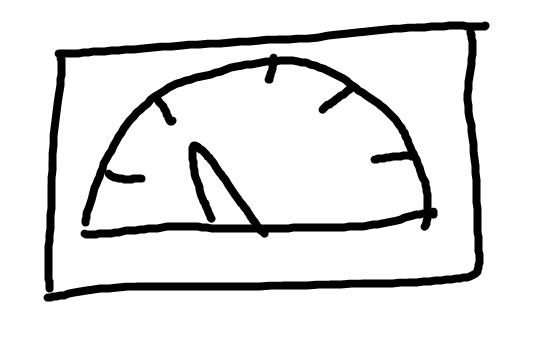
\includegraphics[width=1cm]{images/referrals_triage/detector.png}\\Detector};
        \node [cloud, above of=model] (retrain) {Retrain};
        \node [cloud, right of=detector, align=center] (detection) {Drift\\detection};
        \node [block, above of=retrain] (ds) {
\includegraphics[width=1cm]{images/referrals_triage/datascientist.png}\\Data scientist};
        % Draw edges
        \path [line] (gp) -- (referral) -- (detector);
        \path [line] (referral) |- (clinician);
        \path [line] (clinician) -- (label) -- (detector);
        \path [line] (referral) |- (model);
        % \path [line] (referral) -- (detector);
        \path [line] (model) -- (prediction) -- (detector);
        \path [line] (detector) -- (detection) |- (ds);
        \path [line] (ds) -- (retrain);
        \path [line] (retrain) -- (model);
        \path [line, dashed] (model) -- (support) -- (clinician);
    \end{tikzpicture}
    \caption{The proposed method for handling concept drift in GP referrals triage.}
    \label{fig:referrals_triage}
\end{figure}

This setting diverges from the standard concept drift problem formulation in that there may be an arbitrarily long delays between new instances arriving and correct labels becoming available. Furthermore, the labels may become available in a different order to instances.

Also, unlike in the standard approach where the detector automatically retrains the model when drift is detected, in the GP referrals context, a human in the loop oversees and assists in model retraining. 

How should a concept drift detector be designed to meet these challenges?

\section{Problem Statement}


% In order to make an informed decision about what action to take, the data scientist will want to know:
% \begin{itemize}
%   \item Has the distribution of referrals changed? And if so, does this require model retraining or recall? Can this be detected before all the labels have arrived, which could take arbitrarily long?
%   \item Will retraining the model on more recent data actually improve its performance? Or is performance irreparably degraded under the new distribution because the referral tasks have become intrinsically more difficult?
%   \item How severe was the concept drift and how long ago did it occur? Can the uncertainty on these questions be quantified?
% \end{itemize}
% Existing drift detector methods are unable to provide this information. This is the problem we intend to solve in this thesis.

% We are interested in applying concept drift detection to a task where instances and labels arrive in an irregular manner, and where model retraining is facilitated by a human expert. The main research questions we explore are:

To assist a human expert in making effectively adapting a model to concept drift, we would like to be answer the following questions:
\begin{enumerate}
  \item If there is a delay between having access to new instances and their corresponding labels, is it possible to get early warnings that the data distribution has changed so that the model is no longer fit for purpose?
  \item Sometimes model performance will degrade {\it irreducibly}, meaning that the average difficulty of the prediction task has become more difficult such that retraining the model will not be useful. Can we differentiate between reducible and irreducible error, so that the human expert can evaluate whether a model performance can be recovered after concept drift?
  \item Given that it is not possible to know exactly when concept drift occurred or how severe it is, can we compute probability distributions over times when drift may have occurred, or over how much a model's performance has degraded due to concept drift? This would allow the expert to make retraining decisions informed by expected utility.
\end{enumerate}

\section{Objectives}

The aims of our research are:
\begin{enumerate}
  \item To develop a system which can provide early warnings of concept drift based on instance values when labels have not yet become available.
  \item To develop drift detection algorithms which only detects reducible, and not irreducible, degradation in performance.
  \item To develop a drift detection method which computes probability distributions for drift timing and model degradation.
\end{enumerate}

\section{Contributions}

The main contributions of our work are:
\begin{enumerate}
  \item A framework for providing early warnings that a model requires retraining or recall, the multiple drift detector (MDD). MDD monitors the instance distribution, the label distribution, and model performance metrics for indicators of concept drift. We also present a graphical interface for visualising the history of the status of MDD.
  \item A drift detector which only detects reducible, and not irreducible, performance degradation, the calibrated drift detection method (CDDM).
  \item A drift detection method which computes which computes probability distributions for drift timing and model degradation, the Bayesian drift detection method (BDDM). Additionally, we introduce beta with adaptive forgetfulness (BWAF), an efficient heuristic approximation of BDDM.
\end{enumerate}

\section{Overview of Research}

\begin{figure}
    \centering
    \tikzstyle{block} = [rectangle, draw, 
    text width=7em, text centered, minimum height=4em]
    \tikzstyle{line} = [draw, -latex']
    \begin{tikzpicture}
        \node [block] (detection) {Concept drift detection};
        \node [left of=detection, node distance=4cm] (left) {};
        \node [right of=detection, node distance=4cm] (right) {};
        \node [block, below of=left, node distance=4cm] (types) {Detecting multiple drift types (Chapter \ref{chapt:MDD}).}; %
        \node [block, below of=detection, node distance=4cm] (reducible) {Detecting drift due to reducible error (Chatper \ref{chapt:CDDM}).};
        \node [block, below of=right, node distance=4cm] (uncertainty) {Quantifying drift uncertainty (Chapter \ref{chapt:BDD}).};
        % Draw edges
        \path [line] (detection) -| (types);
        \path [line] (detection) -- (reducible);
        \path [line] (detection) -| (uncertainty);
    \end{tikzpicture}
    \caption{Overview of the topics covered in this thesis.}
    \label{fig:overview_topics}
\end{figure}

The topics discussed in this thesis are illustrated in Figure \ref{fig:overview_topics}. To understand how our contributions would assist the human expert in adapting the decision support system of our motivating example to concept drift, consider Figure \ref{fig:human_decision_flow}. 

If the distribution of instances changes, MDD will provide an early warning that ``feature drift" has occurred. The expert inspects the distributional change using the MDD graphical interface, and decides whether the instance distribution has changed sufficiently that the model is no longer fit for purpose. If it the model is not fit for purpose, then it is recalled from the decision support system, so that it is not contributing clinically harmful predictions. Otherwise, no action is required.

If the relationship between instances and labels changes (i.e., if the triaging rules change), then MDD will warn that concept drift has occurred. At this point, the expert can consult the BDDM for a probability distribution over performance metrics, to determine if the model has sufficiently degraded to require retraining. 

If the model {\it does} require retraining, then the expert can consult CDDM for whether the degradation is reducible or irreducible. If the change is irreducible, then by definition, model retraining will not recover model performance and the model must be recalled from the decision support system. If the degradation {\it is reducible}, then the expert can again consult BDDM for a probability distribution over drift timing. With this information, the expert can determine a suitable data set to retrain the model. If the retrained model performs adequately, then it can re-deployed in the decision support system.

\begin{figure}
    \centering
    
    % Define block styles
    \tikzstyle{decision} = [diamond, draw, fill=blue!20, 
        text width=4.5em, text badly centered, node distance=3cm, inner sep=0pt]
    \tikzstyle{block} = [rectangle, draw, fill=green!20, 
        text width=5em, text centered, rounded corners, minimum height=4em]
    \tikzstyle{line} = [draw, -latex']
    \tikzstyle{cloud} = [draw, ellipse,fill=red!20, node distance=3cm,
        minimum height=2em]
        
    \begin{tikzpicture}[node distance = 2cm, auto]
        % Place nodes
        % real drift flow
        \node [block] (real) {Real drift};
        \node [decision, below of=real] (posterior) {Fit for purpose};
        \node [decision, below of=posterior] (reducible) {Is error reducible?};
        % feature drift flow
        \node [block, left of=real, node distance=3cm] (feature) {Feature drift};
        \node [decision, left of=reducible, node distance=3cm] (fit) {Fit for purpose?};
        % outcomes
        \node [cloud, below of=fit, node distance=3cm] (recall) {Recall};
        \node [cloud, left of=recall, node distance=3cm] (continue) {No action};
        \node [cloud, below of=reducible, node distance=3cm] (retrain) {Retrain};
        % Draw edges
        \path [line] (feature) -- (fit);
        \path [line] (fit) -- node {no} (recall);
        \path [line] (fit) -- node {yes} (continue);
        \path [line] (real) -- (posterior);
        \path [line] (posterior) -- node {no} (reducible);
        \path [line] (posterior) -| node [above] {yes} (continue);
        \path [line] (reducible) -- node {yes} (retrain);
        \path [line] (reducible) -- node {no} (recall);
    \end{tikzpicture}
    \caption{The decision making of the human expert.}
    \label{fig:human_decision_flow}
\end{figure}


\section{Structure of this Thesis}

This thesis is structured into the following chapters.
\begin{itemize}
    \item Chapter \ref{chapt:Background} provides background on machine learning and data streams, and surveys related work on concept drift detection.
    \item Chapter \ref{chapt:MDD} introduces multiple drift detector (MDD), a framework  for providing early warnings that a model requires retraining or recall.
    \item Chapter \ref{chapt:CDDM} introduces calibrated drift detection method (CDDM), a drift detector which only detects reducible, and not irreducible, performance degradation.
    \item Chapter \ref{chapt:BDD} introduces Bayesian drift detection method (BDDM), a method for exactly calculating posterior probabilities of drift timing and performance degradation. We also introduce beta with adaptive forgetfulness (BWAF), an efficient heuristic approximation of BDDM.
    \item Chapter \ref{chapt:Experiments} describes experiments in which validate our novel drift detection methods. These involve a Bernoulli data stream, a battery of benchmark data streams, and a synthetic GP referrals triage data stream.
    \item Chapter \ref{chapt:Conclusion} concludes this thesis by summarising the key points and discussing directions for future research.
\end{itemize}

\chapter{Background} \label{chapt:Background}

In this chapter we provide background and related work for this thesis. Section \ref{background:setting} introduces the setting of this work in machine learning and data streams, including notation and definitions. Section \ref{background:related_work} discusses the related work on concept drift. Section \ref{background:conclusion} summarises the related work.

%-------------------------------------------------------------------
% SETTING
%-------------------------------------------------------------------

\section{Setting} \label{background:setting}

In this section we outline the setting of this thesis. Specifically, we provide the definitions and notation which will be used to describe machine learning and data streams.

% In Section \ref{setting:ml} we give notation and definitions relating to machine learning.  In Section \ref{setting:data_streams} we give notation and definitions relating to data streams.  

% \subsection{Machine Learning} \label{setting:ml}

% \newcommand{\y}[1]{y^{(#1)}}
% \newcommand{\yhat}[1]{\hat{y}^{(#1)}}
% \newcommand{\q}[1]{q^{(#1)}}
% \newcommand{\qhat}[1]{\hat{q}^{(#1)}}
\newcommand{\id}[1]{\mathds{1}[#1]} % identity function
\newcommand{\x}[1]{x^{(#1)}}
\newcommand{\X}[1]{X^{(#1)}}
% \newcommand{\qyhat}{\q{\hat{y}}}

A {\bf label} is a random variable to be predicted by the machine learning model, denoted $y\in dom(y)$. In general, a label may be (non-exhaustively) binary, numeric, or categorical. However, in this thesis we will only be concerned with binary and categorical labels.\footnote{An astute reader will note that we equivocate between $y$ being a random variable and $y$ being a specific value {\it of} that variable, and similarly with $x,q,z$, etc. This is to simplify notation.}  

A {\bf binary label} may only take the values $0$ and $1$. We will denote binary labels with $y$. Because this is also the symbol for a generic label, we will explicitly note when a label is binary. A {\bf multiclass label} may take on any of $n$ values, $dom(y)=\{c_1,c_2,\dots,c_n\}$. %We denote a multiclass label as a one-hot vector ${\bf y}=(y^{(1)},y^{(2)},\dots,y^{(n)})$, where $y^{(i)}=\id{y=c_i}$, and $\id{}$ is the identity function. For example, if $dom(y)=\{cats, dogs, pigeons\}$, and $y=pigeons$, then
% \begin{equation}
%     \bf{y} = \begin{pmatrix}y^{(0)}\\y^{(1)}\\y^{(2)}\end{pmatrix} = \begin{pmatrix}0\\0\\1\end{pmatrix}
% \end{equation}

An {\bf instance} is a vector concatenation of one or more variables called {\bf features}, and is denoted $x\in dom(x)$. Features may be (non-exhaustively) binary, numeric, categorical, or free text, and an instance may have any combination of feature types. The $n$-th feature of an instance is denoted $\x{n}$.

A {\bf concept} is a joint probability of instances and labels:
\begin{equation}
    \Pr(x,y).
\end{equation}
It is often convenient to express this in terms of a ``true" relationship between instances and labels, plus some amount of noise, as in:
\begin{equation}
    y = f(x) + \epsilon(x)
\end{equation}
where $f$ is the {\bf relationship}, and $\epsilon$ is {\bf noise} random variable which may or may not vary with $x$. 

The marginal probabilities of labels and instances are called the {\bf label distribution} and the {\bf instance distribution}, and denoted
\begin{equation}
    P(y) \text{ and } P(x).
\end{equation}
 
% The {\bf conditional label distribution} is the probability distribution over labels, conditional on the corresponding instance. For a binary label $y$, we denote conditional label distributions with
% \begin{equation}
%     q = \Pr(y=1|x).
% \end{equation}
% For a multiclass label we use
% \begin{equation}
%     \bf{q} = \begin{pmatrix}q^{(0)}\\q^{(1)}\\\vdots \\q^{(n)}\end{pmatrix} =\begin{pmatrix}\Pr(\y{0}=1|x)\\\Pr(\y{1}=1|x)\\ \vdots\\\Pr(\y{n}=1|x) \end{pmatrix}.
% \end{equation}
% Because the classes are mutually exclusive, we require
% \begin{equation}
%     \|{\bf q}\|_1=\sum_{i=0}^n \q{i} =1.
% \end{equation}
A {\bf learner} is an algorithm designed to infer from a set of instance label pairs a {\bf model} which approximates the relationship between instances and labels. The output of a model is called a {\bf prediction} and is denoted $\hat{y}$. 

There are two kinds of predictions we are concerned with. The first is a {\bf point prediction}, in which the model simply outputs the prediction $\hat{y}$.  
% \begin{equation}
%     \hat{y} = \hat{f}(x) \approx f(x)
% \end{equation}
% or in the multiclass case
% \begin{equation}
%     {\bf \hat{y}} = \hat{f}(x) =  \begin{pmatrix}\yhat{0}\\\yhat{1}\\ \vdots\\\yhat{n} \end{pmatrix} = \begin{pmatrix}\id{\hat{y}=c_0}\\\id{\hat{y}=c_1}\\ \vdots\\\id{\hat{y}=c_n} \end{pmatrix} = \hat{f}(x) \approx {\bf y}.
% \end{equation}
~The second is a {\bf probabilistic prediction}, in which the model outputs a probability distribution over possible labels. 

Due to noise, stochasticity, or the limited inferential capabilities of the learner, there is some probability that the model will make the wrong prediction. We thus denote
\begin{equation}
q = \Pr(y=\hat{y})
\end{equation}
as the {\bf reliability} of the model, or the probability that the model will make the correct prediction, for the given instance. 

For a model which makes probabilistic predictions, the {\bf confidence} is the probability assigned by the model to its predicted label, denoted
\begin{equation}
\hat{q} = \hat{\Pr}(y=\hat{y}).
\end{equation}
The {\bf residual} of a prediction is a metric of the disparity between predictions and labels. For our purposes, it is given by
\begin{equation}
    res = \id{y=\hat{y}} = \begin{cases} 1 & \text{if }y=\hat{y} \\ 0 & \text{if }y\ne\hat{y}.
    \end{cases}.
\end{equation}

% \begin{equation}
%     \hat{q} = \hat{f}(x) \approx \Pr(y=1|x).
% \end{equation}
% or in the multiclass case
% \begin{equation}
%     {\bf \hat{q}} = \hat{f}(x) =  \begin{pmatrix}\qhat{0}\\\qhat{1}\\ \vdots\\\qhat{n} \end{pmatrix} \approx {\bf q}.
% \end{equation}
% The {\bf risk} of a model is the probability of an incorrect prediction:
% \begin{equation}
%     R = P(y=\hat{y}) = \int P(\hat{y}\ne y|x)dP(x)
% \end{equation}
% where $\int f(x) dP(x)$ is the Lebesgue-Stieltjes integral. We use it for the convenience of indicating that $x$ may be discrete or continuous. If $y$ is a binary variable, then we have
% \begin{align}
%     P(\hat{y}\ne y|x) =& P(\hat{y}\ne f(x)=y|x) \\
%     &+ P(\hat{y}=f(x)\ne y|x).
% \end{align}
% The first term is {\bf reducible error}, and can be corrected with further learning. The second term is {\bf irreducible error} and cannot be corrected.

% \subsection{Data Streams} \label{setting:data_streams}

A {\bf time series} is a sequence of values which become successively available as time progresses. We denote these as
\begin{equation}
    Z = z_0,z_1,z_2,\dots
\end{equation}
A {\bf Bernoulli time series} consists of samples of a random variable where:
\begin{equation}
    z_i = \begin{cases}
    1 & \text{with probability $p$} \\
    0 & \text{with probability $1-p$}
    \end{cases}
\end{equation}
where $p$ is the {\bf rate} of the series. The rate of the residual series is called the {\bf error rate} of the model. 

The times at which each value in the time series becomes available are denoted by
\begin{equation}
    \tau_0,\tau_1,\tau_2,\dots
\end{equation}
If the differences in time between all instances are equal, or formally
\begin{equation}
    \tau_{i+1}-\tau_{i} = c
\end{equation}
for all $i\in\mathbb{N}$ and some constant $c$, then the time series is an {\bf evenly spaced time series}. Otherwise it is an {\bf unevenly spaced time series}. 

An example of an evenly spaced time series is hourly measurements of air quality \cite{ME}. An example of an unevenly spaced time series is our motivating example of GP referrals triage, in which new referral documents or clinician labels may become available at any time.

Some specific time series we are interested in are {\bf instance series} or {\bf feature series}, 
the {\bf label series},
the {\bf prediction series},
and the {\bf residual series}, which are denoted, respectively,
\begin{align}
    X &= x_0,x_1,x_2\dots \\
    Y &= y_0,y_1,y_2\dots \\
    \hat{Y} &= \hat{y}_0,\hat{y}_1,\hat{y}_2\dots \\
    RES &= res_0,res_1,res_2\dots
\end{align}
An instance time series and a label time series together are called a {\bf data stream}. A {\bf drift} is a change in the distribution of a series
\begin{equation}
    \Pr_t(z) \ne \Pr_{t+1}(z) \label{eq:drift}
\end{equation}
where $\Pr_t(z)$ is the distribution of $z$ at time $t$. The point at which a drift occurs is called a {\bf drift point} or {\bf drift location}. In Equation \ref{eq:drift}, the drift point is $t+1$.

% For a Bernoulli stream, we call the difference between the rate of the stream before and after the drift the {\bf magnitude} or {\bf severity} of the drift. 

Concept drift is any change in the joint distribution of instances and labels.
\begin{equation}
    \Pr_t(x,y) \ne \Pr_{t+1}(x,y) 
\end{equation}
There are several sub-types of concept drift. Note that there are many variations in the terminology used to describe concept drift \cite{dataset_drift}\cite{characterizing_drift}, so the definitions provided here are not universal. {\bf Feature drift},  also known as and {\bf virtual drift} or {\bf instance drift}, is a change in the distribution of feature values. 
\begin{equation}
    \Pr_t(x) \ne \Pr_{t+1}(x) 
\end{equation}
{\bf Label drift} is a change in the distribution of label values.
\begin{equation}
    \Pr_t(y) \ne \Pr_{t+1}(y) 
\end{equation}
{\bf Real drift} is a change in the distribution of labels conditional on instances. These are the most consequential type of concept drift as they can require a change in the decision boundary of the model.
\begin{align}
    \Pr_t(y|x) \ne \Pr_{t+1}(y|x)
\end{align}
These types of concept drift are not mutually exclusive, and in fact will often occur together. 

We further differentiate feature drift into {\bf on-manifold} and {\bf off-manifold} feature drift. In on-manifold feature drift, the relative probability of instance values increase or decrease, but the set of possible instance values remains the same. In off-manifold feature drift, the set of possible instances changes. For example, in the domain of classifying emails into spam and non-spam, if a new type of ``Nigerian prince" spam email begins circulating, then this is off-manifold feature drift. Conversely, if the relative frequency of ``Nigerian prince" spam email increases from one in one thousand to one in one hundred, then this is on-manifold drift. 

A rich taxonomy of different types of drift has been explored, as illustrated in Figure \ref{fig:drift_taxonomy}. For our purposes, we need only differentiate between {\bf abrupt} drift, where the stream distribution changes from one stable distribution to another stable distribution over a short period of time, and {\bf gradual} drift, where the data stream goes through many ``intermediate distributions" over a long period of time before stabilising on a new distribution.

\begin{figure}
    \centering
    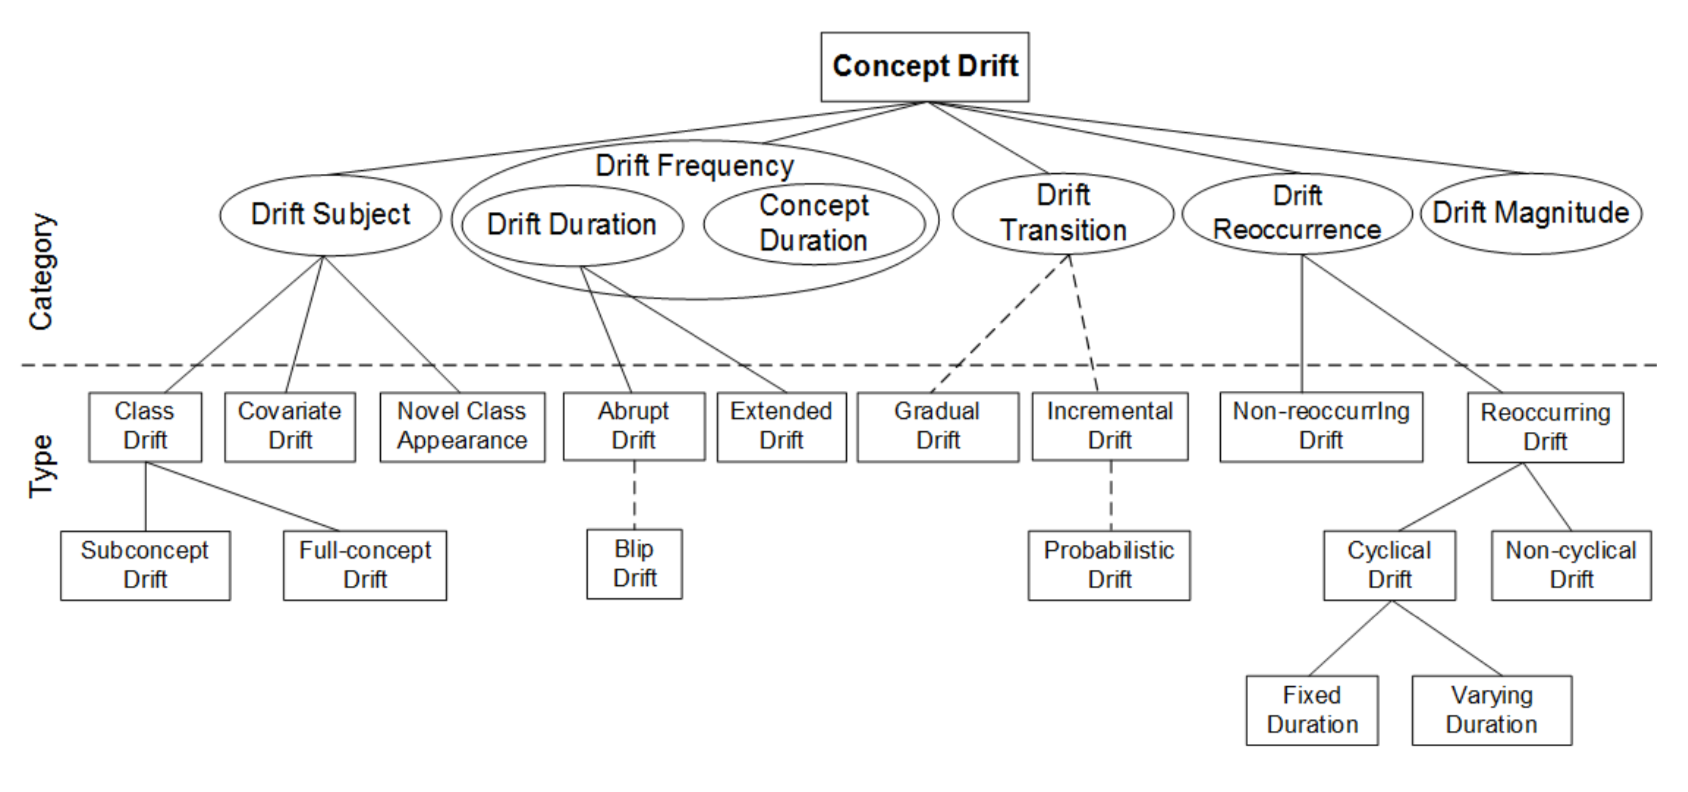
\includegraphics[width=\textwidth]{images/drift_taxonomy.png}
    \caption{Taxonomy of drift types. Solid lines denote mutually exclusive subcategories. Dashed lines denote non-mutually exclusive subcategories. Illustration originally appeared in Webb et al. \cite{characterizing_drift}.}
    \label{fig:drift_taxonomy}
\end{figure}


%-------------------------------------------------------------------
% RELATED WORK
%-------------------------------------------------------------------

\section{Related Work} \label{background:related_work}

There are broadly two approaches to handling concept drift. {\bf Blind} approaches do not explicitly model drift, instead allowing the model to gradually adapt to the new environment. {\bf Informed} approaches, instead employ {\bf drift detectors} to explicitly detect when concept drift has occurred so that the model can be retrained on data from the drift point onward \cite{gama_survey}.

A drift detector is an algorithm which predicts whether drift has occurred for a given data stream
\begin{equation}
    D(Z) \approx \begin{cases}
    1 & \text{if drift has occurred on $Z$} \\
    0 & \text{otherwise}
    \end{cases}
\end{equation}
The following are desirable properties for a drift detector:
\begin{itemize}
    % \item A detector should ideally be {\bf transparency} This enables practitioners to both understand the shortcomings of the model and identify when it is going wrong, and also should allow them to trust the system more, given they can actually see its internal mechanisms.
    \item {\bf Adaptiveness} The ability to detect when concept drift has occurred in a short span of time so that model retraining can commence quickly.
    \item {\bf Accuracy} The system should have a low rate of false-positives and false negatives, so that unnecessary training isn't invoked, and necessary training isn't neglected.
    \item {\bf Robustness} The system should be robust to noise.
\end{itemize}
We now present a survey of the field of concept drift detection research.

% \section{Theoretical Results Pertaining to Concept Drift}
% Holembold and Long (1991, 1994) provide an algorithm which is adaptable to drift up to a given extent.
% Kuh , Petsche, and Rivest (1991, 1994) provide an algorithm and theoretical guarantees for a maximum rate of drift. Their approach is based on the PAC framework.

\subsection{Early Algorithms}

Page \cite{CUSUM} introduced the field of change detection, the parent field of concept drift detection. Page proposed the Page-Hinkley Test (PHT), also known as CUSUM algorithm, in the context of industrial quality control. We imagine testing fixed-size samples of some product from various batches. The number of faulty products from batch $i$ is given by $x_i$. We would like to raise the alarm that the industrial process has gone awry whenever the following condition is met:
\begin{equation}
    \begin{cases}
        x_n > 1 & \text{or} \\
        x_n + x_{n-1} > 2 & \text{or} \\
        \vdots \\
        \sum_{i=0}^k x_{n-i} > k + 1 & \text{for some $k$}
    \end{cases}
\end{equation}
This is equivalent to recording the cumulative sum $S_n = \sum_{i=0}^n x_i$ and raising the alarm whenever
\begin{equation}
    S_n - \min_{i} S_i > h
\end{equation}
for some $h$. In practice, this means we need only keep two registers. First, $S_n$ which accumulates $x_i$, and $S_{min}$, which stores the minimum value of $S_i$ encountered so far.

% This equation can easily be adapted to detect significant deviations in both the positive and negative directions. CUSUM may therefore be used to detect change in any real-valued time series. It can also be used to detect changes in a binary-valued series, if the series is processed in batches, as in the motivating example. 

Work on concept drift often describes adaptations of CUSUM to the problem of concept drift detection \cite{barros_comparison}\cite{gama_survey}. These works cite the original paper by Page \cite{CUSUM}, making the author of these variations unclear. %I have elected to describe the original form of the algorithm as it is more elegant and theoretically justified than its variations.

The study of concept drift {\it per se} appears to originate with the STAGGER algorithm \cite{STAGGER}. This work was heavily influenced by cognitive psychology, so the original usage of ``concepts drift" denoted changes in conjunctive definitions of words. For example, a concept drift could be {\tt bachelor = unmarried AND man} changing to {\tt bachelor = unmarried AND woman}. This work also introduced the STAGGER dataset, which has become a standard benchmark in the field. 

The FLORA family of algorithms  \cite{FLORA}\cite{FLORA2}\cite{FLORA3} expanded the study of symbolic concept drift, and introduced many ideas to the field including recurring concepts, sliding windows of recent examples, and dynamic changes to the window size depending on the stability of the concepts. 

Klinkenberg and Joachim subsequently expanded the study of concept drift to real-valued domains \cite{SVM_detection}. Their approach was to train an SVM online, using a sliding window whose size is chosen to minimise generalisation error, which is estimated with the $\zeta\alpha$ metric. Although this approach was efficient and theoretically well motivated, it was tied specifically to SVMs, and so was not a general solution to the problem of concept drift detection.

The sequential probability ratio test (SPRT) \cite{SPRT} detects when a time series drifts from one distribution $P_1(z)$ to a new distribution $P_2(z)$. Let $z_1,z_2,\dots,z_n$ be some sequence. SPRT monitors the metric
\begin{equation}
  T_1^n = \log\frac{P_1(z_1,z_2,\dots,z_n)}{P_2(z_1,z_2,\dots,z_n)} = \sum_{i=1}^n \log\frac{P_1(z_i)}{P_2(z_i)}
\end{equation}
When $T_1^n>L$, for some parameter $L$, SPRT signals that drift has occurred.

\subsection{Drift Detection Method}

Drift detection method (DDM) \cite{DDM} maintains a running observed mean of the residual time series $p$. The uncertainty around the true error rate is estimated via a normal distribution (the true posterior is a beta distribution) with standard deviation $s=\sqrt{p(1-p)/i}$. A register of the lowest values of $p$ and $s$ are maintained, denoted $p_{min}$ and $s_{min}$. If $s+p>s_{min}+2\cdot s_{min}$, DDM emits a drift warning, and all new instances from that point are stored in a buffer. If $s+p>s_{min}+3\cdot s_{min}$, DDM emits a signal that drift has occurred, and the model is retrained on the instances in the buffer. 

RDDM \cite{RDDM} is a variant of DDM with periodic resets to become more reactive to changes in the error-rate. EDDM \cite{EDDM} is another variant, which monitors for changes in the distribution of {\it gaps} between errors, rather than changes in the error rate itself.

\subsection{Sliding Window Methods}

STEPD essentially approaches concept drift detection by testing the hypothesis ``the error-rate changed $n$ time steps ago for some fixed, and pre-set $n$" at each time step \cite{STEPD}. This is achieved by partitioning the data stream history into 1) a sliding window of the most recent $n$ values, and 2) the preceding values. The statistical test of equal proportions is then used to test whether the rates of the two partitions are significantly different.

FTDD , FPDD, and FSDD \cite{FTDD} are variants of STEPD, which uses Fischer's exact test %or the chi-square test 
in place of the test of equal proportions, because the latter is inappropriate for small or imbalanced data. 

WSTD is another variant, which uses the Wilcoxon rank sum statistical test instead of the test of equal proportions, and additionally limits the size of the second partition \cite{WSTD}.

PL (paired learners) is another sliding window method \cite{PL}. However, rather than testing for differences in error rates of a single model between the two partitions, it instead tests for differences in the error rates of two models. One model, the ``stable learner" is trained online on the entire data stream, and the other, the ``reactive learner" is trained only on the contents of the sliding window. If the proportion of instances in the window that are classified correctly by the reactive learner, but not the stable learner, exceeds some threshold, then drift is indicated.

FHDDM may be considered a hybrid of DDM and sliding window methods \cite{FHDDM}. At each time step the error rate in the sliding window is estimated. If this error rate significantly exceeds its lowest value, then drift is indicated.

SEQDRIFT2 \cite{seq_drift} uses the Bernstein bound to compare a window of the most recent instances with a reservoir of the preceding instances.

MDDM \cite{MDDM} uses both a sliding window {\it and} geometric or linear weighting, and uses the McDiarmid bound. It detects increases in the weighted error rate in the window.

\subsection{Adaptive Windowing}

A major flaw of the sliding window approaches is that they are brittle with respect to the window size parameter. If the window size is too large then there will be a large delay in the drift detection. If the window is too small then the detector will not be able to detect small drifts over random noise. ADWIN combats this problem by dynamically increasing or decreasing the window size \cite{ADWIN}. The authors explain:
\begin{displayquote}
    The idea is simple: whenever two ``large enough" subwindows of $W$ exhibit ``distinct enough" averages, one can conclude that the corresponding expected values are different, and the older portion of the window is dropped. In other words, $W$ is kept as long as possible while the null hypothesis ``$\mu_t$ has remained constant in $W$" is sustainable up to confidence $\delta$.
\end{displayquote}
This involves testing for drift at each time step in the window, which requires a multiple comparisons correction. One of the main advantages of ADWIN is that it provided theoretical guarantees on its false positive and negative rates.

SEED \cite{SEED} is another drift detection method which considers multiple drift points. Unlike ADWIN, the data are processed in batches or ``blocks", so most possible drift points are automatically excluded. When contiguous blocks are evaluated via the Hoeffding inequality to have the same rate, then the two are merged, thus eliminating one potential drift point.

\subsection{EWMA}

An exponentially weighted moving average (EWMA) \cite{EWMA} is an estimation of a variable $x$, which gives exponentially more weighting to more recent examples:
\begin{equation}
  \hat{x}_t = \lambda \hat{x}_{t-1} + (1-\lambda) x_t
\end{equation}
where $\lambda$ is the decay factor. EWMA is employed in several drift detection methods as it provides a way of estimating the current error rate of the model without knowing how far back in time a drift occurred. When the EWMA estimation of the error rate is significantly larger than the overall mean error rate, then we may conclude drift has occurred. ECDDM is a straightforward application of EWMA to concept drift detection, deriving p-values from a lookup table \cite{ECDDM}. LFR also uses EWMA, although p-values are derived from Monte Carlo estimation \cite{LFR}.

\subsection{HDDM}

Fr{\'\i}as-Blanco et al. \cite{HDDM} cast the drift detection problem as follows. There are $n$ examples $x_1,\dots,x_n$, and a hypothesised drift point $d$. The instances before the drift point are denoted $X=x_1,\dots,x_{d-1}$, and their mean is denoted $\mu_X$. Similarly, those instances after the drift point are denoted $Y=x_d,x_{d+1},\dots,x_n$, and their mean $\mu_Y$. These means are estimated using either the sample average or exponentially weighted average. Depending on which estimator is used, the method is known as HDDM$_A$ or HDDM$_W$. The estimations are denoted $\hat{\mu}_X$ and $\hat{\mu}_Y$, respectively. The authors derive bounds for $P(\hat{\mu}_X+\epsilon < \hat{\mu}_Y|\mu_X \ge \mu_Y)$ and $P(\hat{\mu}_X > \hat{\mu}_Y|\mu_X+\epsilon < \mu_Y)$, thus bounding the false positive and false negative rates, respectively.

This is incorporated into an online drift detection algorithm as follows. At time $t$, the hypothesised drift point is set to $d=t$, and is fixed at this value until enough instances are accumulated to the right of the drift point that either $P(\hat{\mu}_X+\epsilon < \hat{\mu}_Y|\mu_X \ge \mu_Y)$ is statistically insignificant, in which case a drift is signalled, or $P(\mu_X+\epsilon < \mu_Y)$ is statistically insignificant, in which case $d$ is set to the current time step. A major advantage of HDDM is that the derived bounds do not assume that the data stream to be monitored is Bernoulli, so can be used to detect drift on real-valued loss streams.

\subsection{Region Drift}

Most of the drift detectors discussed so far have supposed that when concept drift occurs, all the data before the drift becomes irrelevant. Liu et al. \cite{LLD} introduced the notion of {\bf region drift}, in which concept drift only affects a ``region" of instance space. Thus all the data outside of this region from before the drift can be reused when retraining the model. The authors present a new drift detector, local drift degree (LLD), which processes data in batches and uses the nearest neighbour methods to determine if drift has occurred in each region since the previous batch.

\subsection{Data Batches}

Degree of drift (DoF) \cite{DoF} considers data in batches. If the most recent two batches have a heterogeneous Euclidean/overlap metric (HEOM) which is $s$ standard deviations above the mean of past batches, then drift is indicated.

\subsection{Unbalanced Classes}

Wang et al. \cite{DDM-OCIa}\cite{DDM-OCIb} argue that most drift detectors, which detect concept drift via monitoring for increases in the error rate are unsuitable for data streams with unbalanced classes, because
\begin{quote}
  the  minority class  contributes  too  little  to  these  performance  measures compared  to  the  majority  class [and]  too  few  examples from the minority classes can make the time arbitrarily long until  the  concept  drift  is  detected.
\end{quote}
Wang et al. thus propose drift detection method for online class imbalance (DDM-OCI). This monitors for decreases in the recall of the minority class, rather than decreases in the overall accuracy of the model.

Linear four rates (LFR) \cite{LFR} expands on this idea. In addition to monitoring the recall of the minority class, it also monitors the recall of the majority class and the precision of both. It uses an EWMA-style \cite{EWMA} estimator with lookup tables to detect changes in these rates.

PerfSim \cite{perfsim} similarly monitors all the components of the confusion matrix, and uses the cosine similarity test to detect changes between batches of data. CSDD \cite{CSDD} uses the same test, but uses a sliding window rather than batches of data.

\subsection{Bayesian Concept Drift Detection}

Many researchers have proposed Bayesian approaches to change point detection, a problem closely related to concept drift detection. Barry and Hartigan \cite{barry_hartigan} derived an $O(n^3)$ algorithm for detecting {\it multiple} change points within a time series. Fearnhead \cite{fearnhead} developed an $O(n^2)$ algorithm to achieve the same task. 

Adams and MacKay \cite{adams_mackay} adopted a Bayesian approach to change point detection for online contexts. This approach considers a hypothesis space of $l=1, l=2, \dots$, where $l=i$ indicates that a drift point occurred $i$ time steps in the past. At each new time step, the posterior $\Pr(l=i)$ for each $i$ is recalculated.

Bach and Maloof \cite{BCMC} adopted the Adams-MacKay approach to concept drift adaptation. They proposed the Bayesian conditional model comparison (BCMC) algorithm, which makes predictions according to an ensemble of Bayesian learners, one for each value of $l=i$. The models are weighted according to the $\Pr(l=i)$ posteriors. The authors also propose a more efficient algorithm which approximates BCMC, called the pruned Bayesian conditional model comparison (PBCMC).

% \subsection{Ensemble approaches}
% ELM \cite{ELM}


% \subsection{Expeirments}

% \cite{barros_comparison}


%-------------------------------------------------------------------
% CONCLUSION
%-------------------------------------------------------------------

\section{Conclusion} \label{background:conclusion}

With some abstraction, we can consider drift detection methods of consisting of three components. First is the method of generating drift point candidates. The common approaches are using a {\it sliding window}, in which case the candidate drift point is the start of the window, {\it aggregation}, in which case the data stream is aggregated into blocks and the spaces between these blocks are used as drift point candidates, {\it batching}, in which the spaces between batches of data are drift point candidates, and {\it thresholding}, in which case the candidate drift point is derived by monitoring for a summary statistic exceeding some threshold.

The second component of a drift detector is a statistical test. Many detectors make use of Hoeffding's test, Bernstein's test, McDiarmid's test, Fischer's exact test, or the cosine test. 

The third component is the operationalisation of concept drift. The general problem of concept drift detection is virtually insoluble in its most general form, so drift detectors operationalise the problem to make it tractable. The most common operationalisation is to detect increases in the error rate of the model. Other approaches include monitoring for increases in the precision and recall.
All the existing drift detectors we have surveyed are summarised according to these components in Table \ref{tab:drift_detectors}.

\begin{table}[]
    \centering
    \caption{Summary of existing drift detectors}
    \label{tab:drift_detectors}
    \begin{tabular}{|l|l|l|l|}
         \toprule
         Detector & Drift Points & Statistical Test & Operationalisation  \\
         \midrule
         ADWIN & aggregation & Hoeffding & Accuracy \\
         CSDD & cosine & batches & Recall, Precision \\
         CUSUM & threshold & - & Accuracy \\
         DDM & threshold & - & Accuracy \\
         DDM-OCI & threshold & - & Recall \\
         DoF & batches & - & Accuracy \\
         ECDDM & threshold & - & Accuracy \\
         EDDM & threshold & Hoeffding & Accuracy \\
         FHDDM & window & Hoeffding & Accuracy \\
         FLORA & - & - & Accuracy \\
         HDDM & window & Hoeffding & Accuracy \\ 
         LDD & batches & - & Accuracy \\
         LFR & threshold & - & Recall, Precision  \\
         MDDM & window & McDiarmid & Accuracy \\
         PerfSim & window & cosine & Recall, Precision \\
         PL & window & - & Accuracy \\
         RDDM & threshold & Hoeffding & Accuracy \\
         SEED & Blocks & Hoeffding & Accuracy \\ 
         SeqDrift2 & window & Bernstein & Accuracy \\
         SPRT & threshold & - & - \\
         STAGGER & - & - & Accuracy \\
         STEPD & window & - & Accuracy \\
         \bottomrule
    \end{tabular}
\end{table}









\chapter{Multiple Drift Detector} \label{chapt:MDD}

In this chapter we introduce multiple drift detector (MDD), a framework for human in the loop detection of multiple types of drift. Section \ref{mdd:motivation} discusses the motivation for MDD. Section \ref{mdd:algorithm} provides the algorithms pertaining to MDD. Section \ref{mdd:graphics} introduces a graphical interface for MDD. Section \ref{mdd:illustration} illustrates the utility of MDD within the medical referrals triage motivating example. Section \ref{mdd:conclusion} summarises this chapter and discusses future work.

%-------------------------------------------------------------------
% MOTIVATION
%-------------------------------------------------------------------

\section{Motivation} \label{mdd:motivation}

There is a standard ``grammar" of concept drift detection methods, in which the problem is formulated according to certain axioms. The import of these axioms varies significantly. Some are universal, others only common. Some are implicit, others explicit. Some are fundamental, others incidental and easily worked around. Some have important consequences, others are trivial. If the axioms do not obtain, then this will limit the applicability of the drift detection method. Below are some axioms we have identified, which are likely to deviate from the reality of practical applications, with discussion of how often they are adhered to:
\begin{itemize}
  \item {\bf Stable instance distribution} - Degradation in model accuracy may occur because 1) the model has gotten worse at predicting labels for specific instances, or 2) the proportion of instances which the model is bad at predicting has increased. Retraining will not necessarily be helpful in the second case, as there may be irreducible error. However, to our knowledge there are no extant concept drift detection methods which account for the possibility of changes in the instance distribution, and try to differentiate the two sources of increased error.
  \item {\bf Immediate labelling} - Labels become available immediately after the model has made its prediction. To our knowledge, there is no work on concept drift which entertains the possibility that this is not the case.
  \item {\bf Indexed time} - Instances arrive at regular time intervals, or periodic batches. % To our knowledge, there is no work on concept drift detection which accounts for instances arriving at irregular intervals.
  \item {\bf No human-in-the-loop} - A human is neither available nor necessary to assist in the model retraining process. To our knowledge, there is no work on human-in-the-loop concept drift detection or adaptation.
  \item {\bf Non-interpretability} - It is not necessary to understand {\it how} the joint feature-label distribution is changing, only to know that it {\it is} changing. Drift detection methods vary in interpretable they render the evolution of a data stream. DDM provides almost no additional information beyond its verdict on whether concept drift has occurred, whereas ADWIN provides p-values for all possible drift points, as well as estimates of the error rates before and after the drift point. %However, none have explicitly held interpretability as a goal.
  \item {\bf Binary labels} - All instances are classified into the positive and negative class.
  \item {\bf Balanced class labels} - Prior to DDM-OCI, concept drift detection work had tended to implicitly assume that labels would be balanced. Since DDM-OCI, LFR and PerfSim have explicitly accounted for labels being potentially unbalanced.
  \item {\bf Efficiency over accuracy} - Concept drift detection is often discussed in the context of data streams, in which computational resources are at a premium due to a high throughput of instances. Some drift detection methods embrace this axiom, such as SEED which uses reservoir sampling. However, there are also detection methods which sacrifice efficiency for accuracy, such as ADWIN.
  \item {\bf Online learning} - To our knowledge, all investigations into concept drift have expected the model to be learning online from new instances as they arise. The possibility of a model being trained and frozen ahead of the data stream on historical instances has not been explored. However, for most drift detection methods this makes no practical difference, so this is not a real impediment.
\end{itemize}

In practical data science, any of these axioms may be violated. As an illustration, we return to our motivating example of  GP referrals triage, and see whether the axioms obtain:
\begin{itemize}
  \item {\bf Stable instance distribution} - The instance distribution is likely to change due to changes in demographic, epidemiological, or other factors. Thus this axiom does not hold.
  \item {\bf Immediate labelling} - There may be a considerable delay between a referral document arriving and it being labelled by a clinician. Arbitrarily many new documents could arrive in this interval.
  \item {\bf Indexed time} - Referrals and labels will arrive at irregular intervals, and will display changes in frequency over time.
  \item {\bf No human-in-the-loop} - Because retraining the model requires coordination by a consulted data scientist, a human is both necessary and available for model retraining.
  \item {\bf Non-interpretability} - Interpretability is crucial so that clinicians and data scientists can make informed decisions about what actions to take after concept drift has been detected.
  \item {\bf Binary labels} - Four priority levels are used to categorically label referral documents.
  \item {\bf Balanced class labels} - Medium-priority labels (2 and 3) are more common than extreme priority labels (1 and 4).
  \item {\bf Efficiency over accuracy} - The throughput of instances is fairly low, on the order of one referral document per hour. A powerful GPU machine is detected to modelling the referral data, so computational resources are available for comprehensive drift detection methods. Furthermore, given the high-stakes nature of medical triage, it is essential to make use of these resources to detect concept drift as precisely as possible.
  \item {\bf Online learning} - The model is pre-trained on historical referral data and frozen prior to deployment on the data stream.
\end{itemize}

This illustrates that existing approaches to concept drift are not necessarily appropriate for practical data science, at least without modification. And in particular, existing methods are certainly not appropriate for our motivating example of GP referrals triage. In the next section, we consider operationalisations of concept drift which will be better suited for practical data science.

\subsection{Operationalisations of Concept Drift} \label{Background:operationalisations}
% NOTE: I intend to move this to Chapter 2, but I include it here because it sets up the next section.

Concept drift is a change in the instance-label joint distribution. That is, concept drift is the event
\begin{equation}
  D(x,y)
\end{equation}
where $D(z)$ denotes a change in the distribution of $z$. Attacking this problem directly is frequently too hard to be directly tractable. The most direct approach would be to apply multidimensional change-point detection methods to the joint distribution. In domains with high-dimensional feature space and complex, non-linear relationships between features and labels, these methods will be infeasible. In general, detecting a change in the joint distribution is strictly harder than modelling the relationship between labels and features to begin with. So the techniques used for change point detection should be at least as sophisticated as those used in modelling the data.

Most drift detection methods therefore operationalise the concept drift detection task. Rather than directly detecting a change in the joint distribution, they instead detect an {\it increase in the error rate}. Under a stable joint distribution, model accuracy should either remain steady, or decrease if the model is learning. We denote this operationalisation as
\begin{equation}
  D(x,y) \Leftarrow D_-(y=\hat{y})
\end{equation}
where $D_-(z)$ indicates a decrease in $\mathds{E}[z]$, and $\Leftarrow$ means ``is operationalised as". We call this the {\bf accuracy operationalisation}. It appears to have been introduced by Widmer and Kubat, and has since been employed in the majority of drift detection methods.

Klinkenberg and Renz expanded on the above operationalisation, and monitor each of accuracy, precision of the positive class, and recall of the positive class for decreases. This can be expressed
\begin{equation}
  D(x,y) \Leftarrow D_-(y=\hat{y}) \vee  D_-(y=1|\hat{y}=1) \vee D_-(\hat{y}=1|y=1)
\end{equation}
where the conjuncts indicate accuracy, precision, and recall, respectively.

Wang et al. argue that if a data stream contains imbalanced classes, then a degradation in the model's ability to predict the minority class will be difficult to detect under the accuracy operationalisation. They propose operationalising concept drift as a) detecting class imbalance, and b) detecting a drop in the recall of the minority class. That is
\begin{equation}
  D(x,y) \Leftarrow D(y) \vee D_-(\hat{y}=m|y=m)
\end{equation}
where $m$ is the minority class.

Wang\footnote{Not the same Wang.} and Abraham note that there are some deleterious changes in a model's confusion matrix which previous operationalisations will fail to detect. For comprehensiveness, they propose monitoring both precision and recall for both classes:
\begin{equation}
  D(x,y) \Leftarrow D_-(y=\hat{y}|y) \vee D_-(y=\hat{y}|\hat{y}).
\end{equation}
We will call this the {\bf precision-recall operationalisation}.

\subsection{Practical Operationalisation}

As mentioned in Section \ref{Background:operationalisations}, there are several operationalisations of concept drift which have been proposed. Which of these is most appropriate for practical data science applications? To answer this, we should consider what our objective is in concept drift detection. Upon detecting concept drift, there are three actions we might want to take
\begin{enumerate}
  \item retrain the model using a (recent) subset of the data if it is no longer fit for purpose, or
  \item recall the model if it is no longer fit-for-purpose and cannot be made so by retraining, or
  \item leave the model as-is if it is still fit-for-purpose despite the concept drift.
\end{enumerate}
In our motivating example of GP referrals triage, each of these could be manifested as:
\begin{enumerate}
  \item The triage decision making process has changed, so the model should be retrained on data since that change.
  \item The model is required to have an accuracy of at least 98\% to be ``clinically safe", but due to irreducible error the accuracy is stuck at 95\%. The model should therefore be recalled.
  \item The model has deteriorated slightly in its ability to distinguish between priority 1 and priority 2 referrals. But because there is little practical consequence in confusing these (the important thing is to accurately classify priority 3 and priority 4 labels), it is decided that the model should remain as-is.
\end{enumerate}
Which of these actions is appropriate will depend on the kind of concept drift which has occurred.
\begin{itemize}
  \item {\bf On-manifold feature drift} If the distribution of instances changes such that some kinds of instances become more prevalent and others less prevalent, but the manifold on which instances exist stays the same, then model performance metrics may degrade, however this may be due to changes in irreducible error, and retraining will probably not be necessary. However, if the performance degrades sufficiently, it may be necessary to recall the model.
  \item {\bf Off-manifold feature drift} If the distribution of instances changes such that new instances are occurring which were not part of the original manifold, then the model will not be able to predict the correct label for these instances and will require retraining.
  \item {\bf Real drift} If the relationship between instances and labels changes, then the model will require retraining.
  \item {\bf Label drift} may indicate that a model requires recall. In the GP referrals triage example, if the model starts predicting the same priority for {\it all} referrals, then it will not be fit-for-purpose.
\end{itemize}
Note that feature and label drift may be detected earlier than real drift. These only require instance and prediction values, whereas detection of real drift requires the labels, which may arrive later.

With these considerations in mind, we suggest operationalising concept drift for practical data science into degradations in precision, recall, {\it or} label drift or feature drift:
\begin{equation}
  D(x,y) \Leftarrow D_-(y=\hat{y}|y) \vee D_-(y=\hat{y}|\hat{y}) \vee D(\hat{y}) \vee D(x).
\end{equation}
We further operationalise feature drift into drift for each of its component features. That is, we assume feature independence.
\begin{equation}
  D(x) \Leftarrow D(\x{0}) \vee D(\x{1}) \vee \dots \vee D(\x{n})
\end{equation}
This operationalisation has the following advantages
\begin{itemize}
  \item Operationalising on class-wise precision and recall provides robustness to class imbalance.
  \item Precision and recall can be easily applied to multi-class labels.
  \item Precision and recall are easily interpreted and are natural metrics for expressing fitness-for-purpose thresholds. For example, a triage drift detector may need to maintain recall of 95\% for maximum priority referrals.
  \item By additionally operationalising on predictions and features, one obtains another ``cross section" of the evolution of the data stream, thus making the drift detector more interpretable.
  \item Because feature drift and label drift can be detected ahead of labels becoming available, one can discover early that a model requires training or recall due to off-manifold feature drift or label drift.
  \item One can determine whether degradation in performance metrics is due to unstable decision boundaries, or due to an unstable instance distributions, by investigating whether feature drift has occurred.
\end{itemize}

We shall call an implementation of this operationalisation a multiple drift detector, as it detects not only real drift, but also feature drift and label drift. In the next section, we consider the question of how to construct a multiple drift detector.

%-------------------------------------------------------------------
% ALGORITHM
%-------------------------------------------------------------------

\section{Algorithm} \label{mdd:algorithm}

Do we need to invent entirely new drift detection methods to implement this operationalisation of concept drift? It turns out, we can construct such a concept drift detector out of the detectors from other operationalisations. Each of the operationalisations we have discussed involved detecting an increase in the expected value of some metric, typically accuracy, precision, or recall. These operationalisations were implemented using a drift detection method, or an algorithm which maps a sequence of metric values to a boolean drift status, given a confidence value. We denoted this as
\begin{equation}
  D_-(Z;\alpha) = \begin{cases}
  true & \text{if $\mathds{E}[z]$ has decreased (with $p<\alpha$)} \\
  false & \text{otherwise}.
  \end{cases}
\end{equation}
where $Z=z_0,z_1,\dots,z_t$ is a sequence of metric values. Often the metric is restricted to binary values, although for some drift detection methods, such as HDDM, it may be real-valued.

We can easily adapt such a drift detection method to instead detect increases in the metric:
\begin{align}
  D_+(Z;\alpha) &:= \begin{cases}
  true & \text{if $\mathds{E}[z]$ has increased (with $p<\alpha$)} \\
  false & \text{otherwise}
  \end{cases} \\
  &:= D_-(1-Z;\alpha)
\end{align}
where $1-Z=(1-z_0),(1-z_1),\dots,(1-z_t)$. Note that in the case that the metric is real-valued, it would be sufficient to use the definition
\begin{equation}
  D_+(Z) := D_-(-Z).
\end{equation}
However, the given definition covers both binary and real-valued metrics.

We can also easily construct a bidirectional drift detection method, which detects both increases and decreases in the metric:
\begin{align}
  D_\pm(Z;\alpha) &= \begin{cases}
  true & \text{if $\mathds{E}[z]$ has increased or decreased (with $p<\alpha$)} \\
  false & \text{otherwise}.
  \end{cases} \\
  &:= D_+(Z;\alpha/2) \vee D_-(Z;\alpha/2).
\end{align}
Note that we have halved the confidence threshold as a Bonferonni correction for multiple comparisons.

Detecting changes in categorical variables can be achieved by detecting changes in the rates of each of the categories:
\begin{align}
  D(Z;\alpha) &:= \begin{cases}
  true & \text{if $P(z)$ has changed (with $p<\alpha$)} \\
  false & \text{otherwise}.
  \end{cases} \\
  &:= D(Z^{(0)};\alpha/n_c) \vee D(Z^{(1)};\alpha/n_c) \vee \dots \vee D(Z^{(n_c)};\alpha/n_c)
\end{align}
where $n_c$ is the number of categories, and $Z^{(i)}=z^{(i)}_0,z^{(i)}_2,\dots,z^{(i)}_t=(z_0=i),(z_1=i),\dots,(z_t=i)$.

Detecting changes in multi-dimensional variables can be achieved by detecting changes in each of the dimensions separately:
\begin{align}
  D(Z;\alpha) &:= \begin{cases}
  true & \text{if $P(z)$ has changed (with $p<\alpha$)} \\
  false & \text{otherwise}.
  \end{cases} \\
  &:= D(Z^{(0)};\alpha/n_d) \vee D(Z^{(1)};\alpha/n_d) \vee \dots \vee D(Z^{(n_c)};\alpha/n_d)
\end{align}
where $n_d$ is the number of dimensions, and $Z^{(i)}=z^{(i)}_0,z^{(i)}_2,\dots,z^{(i)}_t$.

Using these compositions, we can construct a multi-drift detector out of an arbitrary base drift detector.

\subsection{Pseudocode}

The multiple drift detector framework essentially consists of five procedures. First, there is the feature preprocessing procedure. This converts categorical features into dummy variables and free text into bag of words representations, so that these features can be processed as a series of binary variables. The preprocessing pseudocode is given in Algorithm \ref{alg:mdd_preprocess}. Second, there is the initialisation procedure for constructing the multiple drift detector out of a base drift detector, following the procedure set out in the previous section. The pseudocode for this is given in Algorithm \ref{alg:mdd_init}. Third, there is the procedure for updating the multiple drift detector when a new instance becomes available, whose pseudocode is given in Algorithm \ref{alg:mdd_instance}. Fourth, there is the procedure for updating the multiple drift detector when a new prediction becomes available, whose pseudocode is given in Algorithm \ref{alg:mdd_prediction}. Finally, there is the procedure for updating the multiple drift detector when a new label becomes available, whose pseudocode is given in Algorithm \ref{alg:mdd_label}. These procedures are tied together in Algorithm \ref{alg:mdd_loop}, which describes the entire updating loop of the multiple drift detector.

Note that this pseudocode  uses a single threshold to indicate when drift has occurred, rather than one threshold for signalling when drift has occurred, and a weaker threshold for delivering a warning that drift may be occurring. This is only for notational convenience. The intention is in fact for multiple drift detector to also have a warning threshold, and one can easily extrapolate from this pseudocode how this will be incorporated.

\begin{algorithm}
    \caption{Preprocess features for multiple drift detector}
    \label{alg:mdd_preprocess}
    \begin{algorithmic}
      \Function{Preprocess}{$\x{0},\x{1},\dots,\x{n}$}
        \Require The domains of each of the features $\X{0},\X{1},\dots,\X{n}$
        \State $x' \gets []$
        \For {$\x{i},\X{i}$}
          \If {$\X{i}=\mathbb{R}$}
            \State $x' \gets x' \cup \x{i}$
            \Comment{Leave real-valued features as-is.}
          \ElsIf {$\X{i}=\{0,1\}$}
            \State $x' \gets x' \cup \x{i}$
            \Comment{Leave binary features as-is.}
          \ElsIf {$\X{i}=k\in \mathbb{N}$}
            \For {i=1,2,\dots,k}
            \Comment{Convert categorical features to dummy variables.}
              \State $x' \gets x' \cup \id{\x{i}=k}$
            \EndFor
          \ElsIf {$\X{i}$ is free-text with vocabulary $V$}
            \For {$v\in V$}
            \Comment{Convert free-text features to bags-of-words}
              \State $x' \gets x' \cup (v\in \x{i})$
            \EndFor
          \EndIf
        \EndFor
      \EndFunction
    \end{algorithmic}
\end{algorithm}

\begin{algorithm}
    \caption{Initialise multiple drift detector}
    \label{alg:mdd_init}
    \begin{algorithmic}
      \Function{Initialise}{}
        \Require Drift threshold $\alpha$
        \Require Instance dimensionality $n_x$
        \Require Number of feature labels $n_y$
        \Require Base drift detector $D_-(Z;\alpha)$
        \State $D_+(Z;\alpha) := D_-(1-Z;\alpha)$
        \Comment Construct each of the drift detectors
        \State $D_\pm(Z;\alpha) := D_-(1-Z;\alpha/2) \vee D_+(Z;\alpha/2)$
        \State $D_x(X) := D_\pm(\X{0};\alpha/4n_x) \vee D_\pm(\X{1};\alpha/4n_x) \vee \dots \vee D_\pm(\X{n_x};\alpha/4n_x)$
        \State $D_y(Y) := D_\pm(\X{0};\alpha/4n_y) \vee D_\pm(\X{1};\alpha/4n_y) \vee \dots \vee D_\pm(\X{n_y};\alpha/4n_y)$
        \State $D_p(P) := D_\pm(\X{0};\alpha/4n_y) \vee D_\pm(\X{1};\alpha/4n_y) \vee \dots \vee D_\pm(\X{n_y};\alpha/4n_y)$
        \State $D_r(R) := D_\pm(\X{0};\alpha/4n_y) \vee D_\pm(\X{1};\alpha/4n_y) \vee \dots \vee D_\pm(\X{n_y};\alpha/4n_y)$
        \State $X, Y, P, R, \hat{Y} \gets [], [], [], [], []$
        \Comment Initialise each of the data streams as empty
        \State $\hat{y}$\_lookup $\gets \{\}$
      \EndFunction
    \end{algorithmic}
\end{algorithm}

\begin{algorithm}
    \caption{Update multiple drift detector when a new instance becomes available.}
    \label{alg:mdd_instance}
    \begin{algorithmic}
      \Function{AddInstance}{$x_t$}
        \State $X\gets X\cup x_t$
        \If {$D_x(X)$}
          \State Signal ``Feature drift"
        \EndIf
      \EndFunction
    \end{algorithmic}
\end{algorithm}

\begin{algorithm}
    \caption{Update multiple drift detector when a new prediction becomes available.}
    \label{alg:mdd_prediction}
    \begin{algorithmic}
        \Function{AddPrediction}{$\hat{y}_t$}
            \State $\hat{Y}\gets \hat{Y}\cup \hat{y}_t$
            \State $\hat{y}$\_lookup$[t] \gets \hat{y}_t$
            \If {$D_y(\hat{Y})$}
              \State Signal ``Label drift"
            \EndIf
        \EndFunction
    \end{algorithmic}
\end{algorithm}

\begin{algorithm}
    \caption{Update multiple drift detector when a new label becomes available.}
    \label{alg:mdd_label}
    \begin{algorithmic}
        \Function{AddPrediction}{$y_t$}
            \State $\hat{y}_t \gets \hat{y}$\_lookup$[t]$
            \State $R^{(y_t)}\gets P\cup \id{y_t=\hat{y}_t}$
            \Comment Update recall
            \State $P^{(\hat{y}_t)}\gets P\cup \id{y_t=\hat{y}_t}$
            \Comment Update precision
            \If {$D_p(P)$ or $D_r(R)$}
              \State Signal ``Real drift"
            \EndIf
        \EndFunction
    \end{algorithmic}
\end{algorithm}

\begin{algorithm}
    \caption{Main loop of multiple drift detector}
    \label{alg:mdd_loop}
    \begin{algorithmic}
        \State \Call{Initialise}{}
        \While {No drift detected.}
          \If {new $x_t$}
            \State $\hat{y} \gets$ model.predict$(x_t)$
            \State $x_t \gets $\Call{Preprocess}{$x_t$}
            \State \Call{AddPrediction}{$\hat{y}_t$}
            \State \Call{AddInstance}{$x_t$}
          \ElsIf {new $y_t$}
            \State \Call{AddLabel}{$y_t$}
          \EndIf
        \EndWhile
    \end{algorithmic}
\end{algorithm}

%-------------------------------------------------------------------
% GRAPHICAL INTERFACE
%-------------------------------------------------------------------

\section{Graphical Interface} \label{mdd:graphics}

As mentioned previously, we would like multiple drift detector to be interpretable, to allow for human-in-the-loop decision making about what action should be taken when concept drift is detected. We therefore implemented a graphical interface for multiple drift detector using Dash, which shows how the data stream and its various metrics are evolving over time. The multiple drift detector records its status with each update to a system of csv files in a user-specified directory, so that the history of the multiple drift detector's state can be graphically rendered.

A screenshot of the interface is shown in Figure \ref{fig:dash_app}. Each of precision, recall, labels, features has a tab in which these data streams can be viewed. For the sake of completeness, there is also a tab in which accuracy over time can be viewed. For each of these data streams, the value is given on the y-axis, and the time index on the x-axis, with smoothing achieved via convolution with a Hanning window of adjustable width. The data points are coloured to indicate the drift status at that point in time. A summary of the status of the multiple drift detector is given in the top right corner of the app, which simply indicates whether concept drift, feature drift, label drift, or real drift are suspected or detected by the multiple drift detector. Within the individual tabs, one is given a break-down of the specific label values or features for which drift has been detected.

\begin{figure}
    \centering
    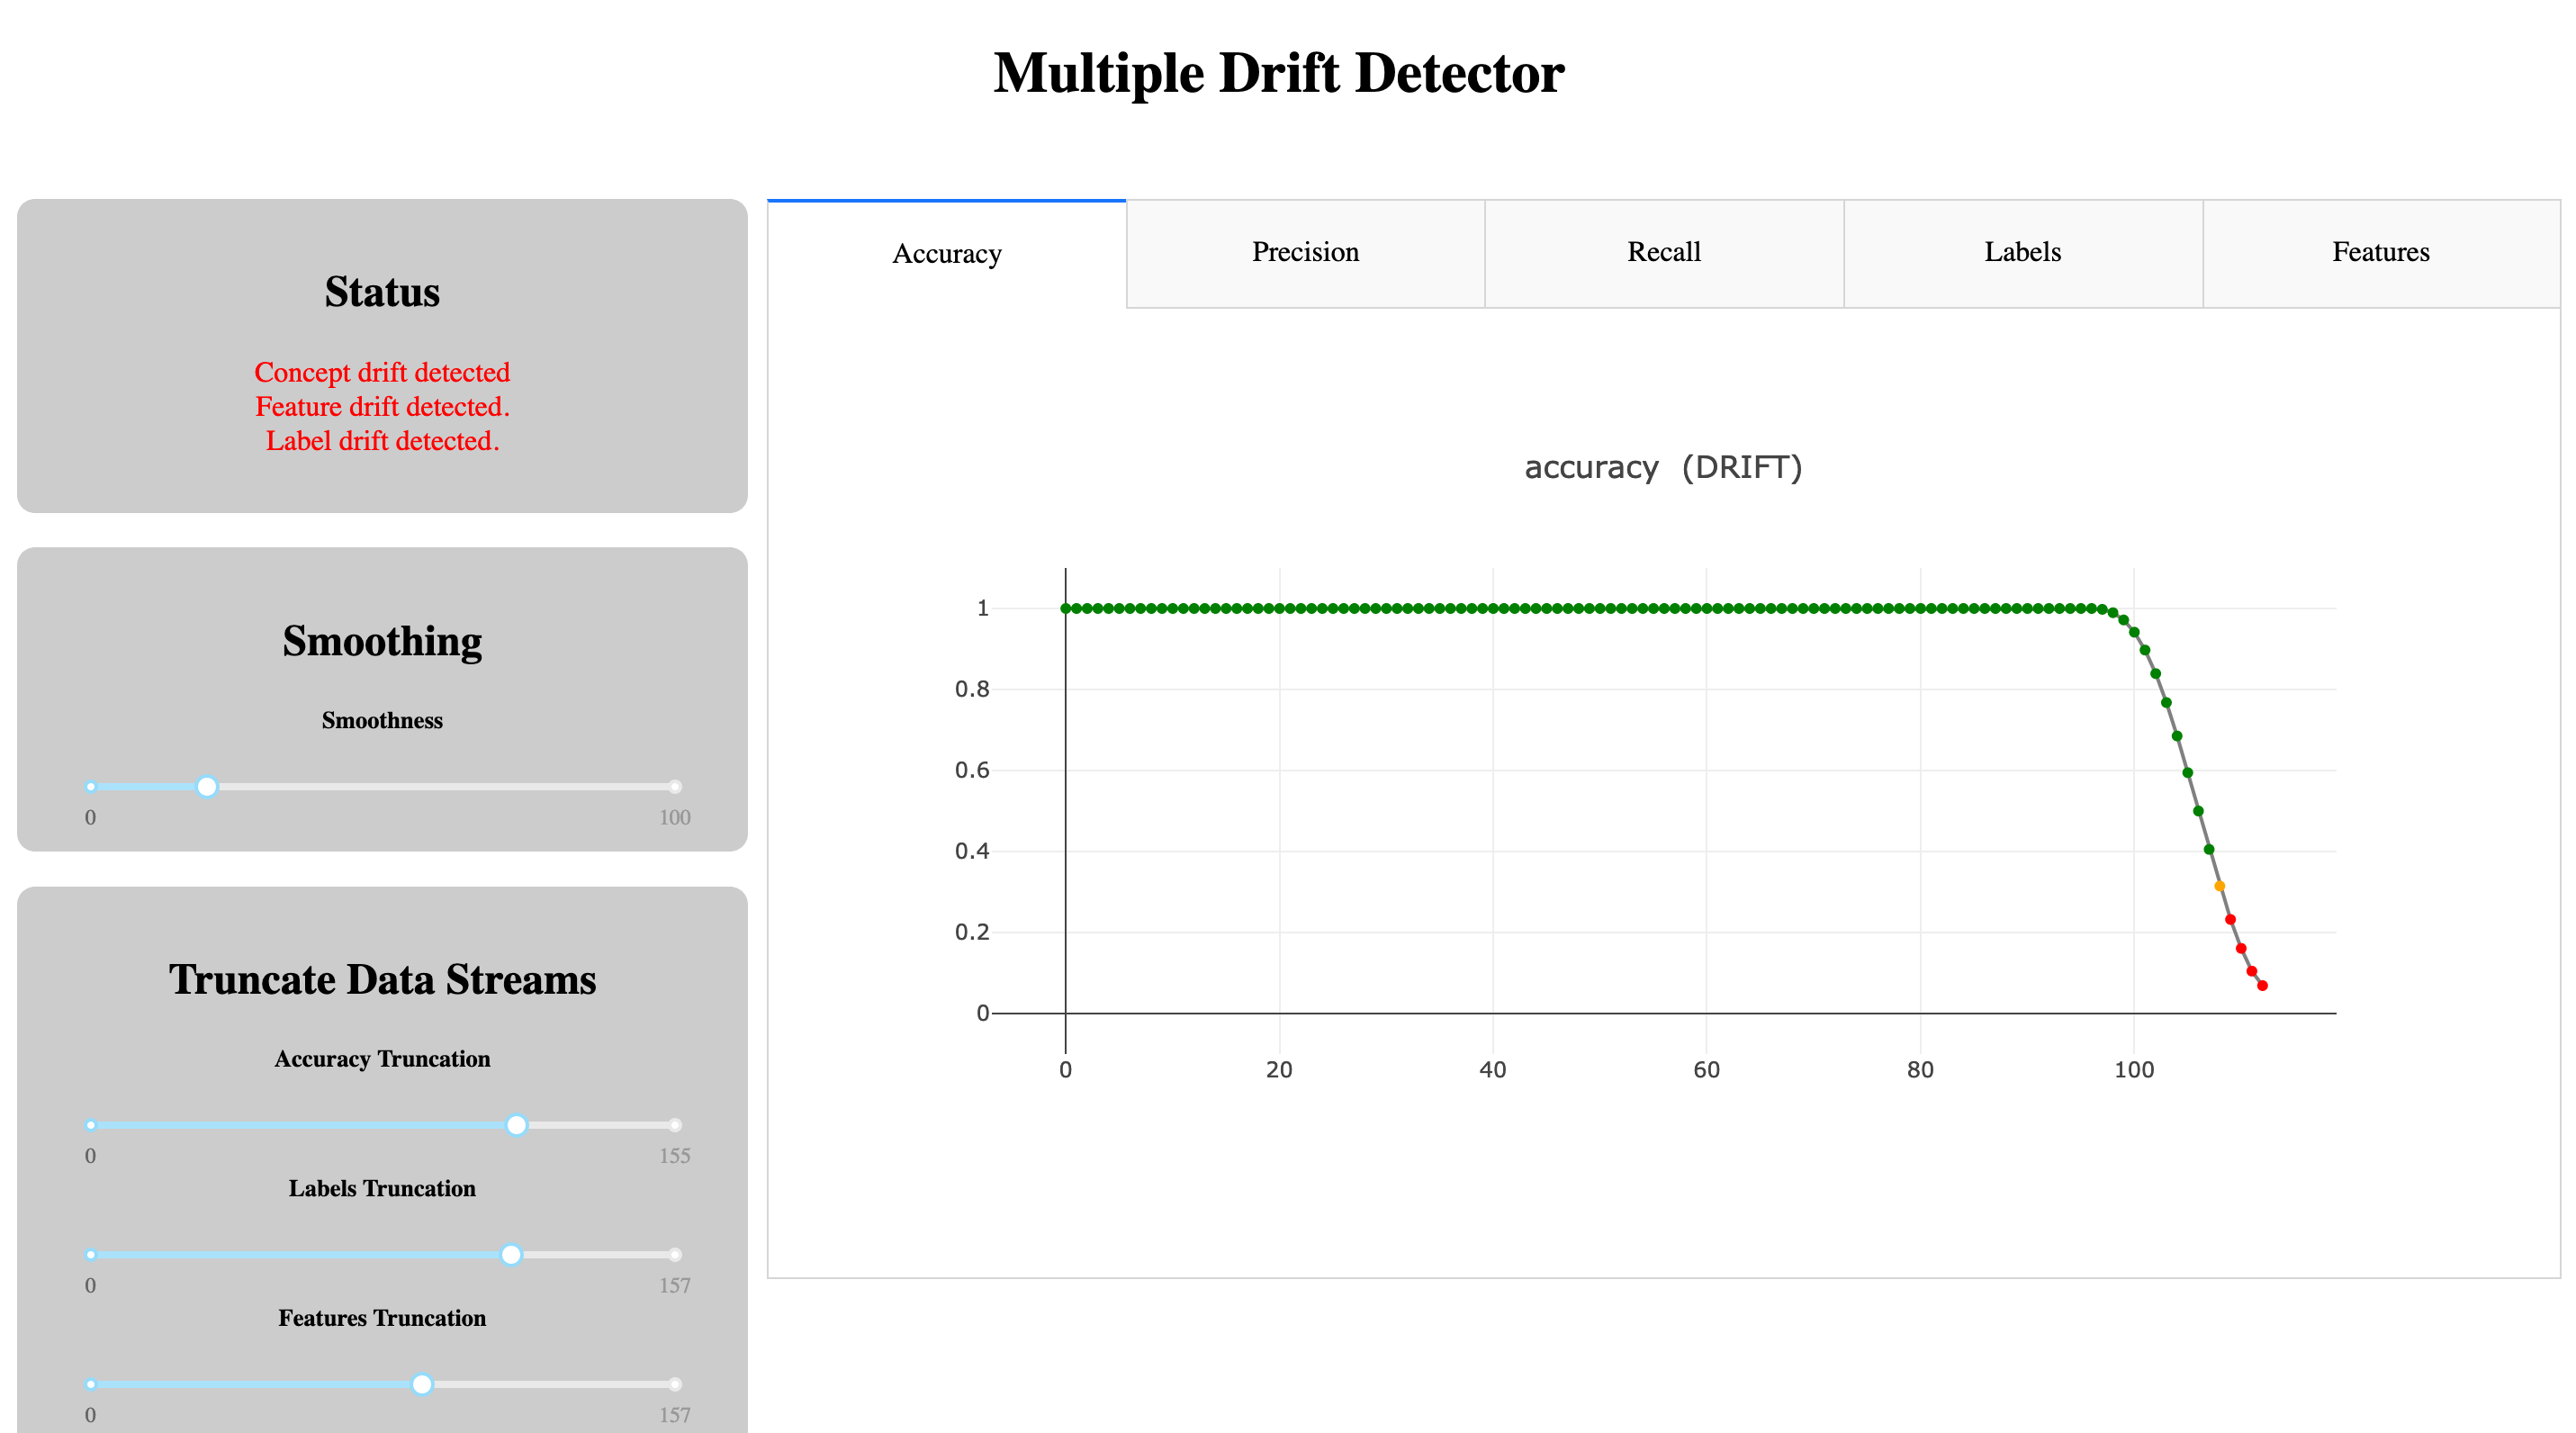
\includegraphics[width=\columnwidth]{images/dash_app.png}
    \caption{The graphical interface for multiple drift detector.}
    \label{fig:dash_app}
\end{figure}

%-------------------------------------------------------------------
% ILLUSTRATION
%-------------------------------------------------------------------

\section{Illustration} \label{mdd:illustration}

In this scenario we illustrate the multiple drift detectors framework using our GP referrals triage motivating example. We explore three drift scenarios, and describe how multiple drift detector will facilitate responding to the drift appropriately. 

\subsection{Scenario 1: Retrain}

Data scientists get a message from the multiple drift detector saying that model recall has decreased for priority 4, and precision has decreased for priority 3, as shown in Figure \ref{fig:scenario1}. Upon investigation, it turns out that a new study has come out that says that coronavirus is more dangerous than previously thought. Patients with this condition are now given priority 4 rather than priority 3.
Data scientists therefore retrain the model on data since the study came out, and the model is once again up to date.

\begin{figure}
    \centering
    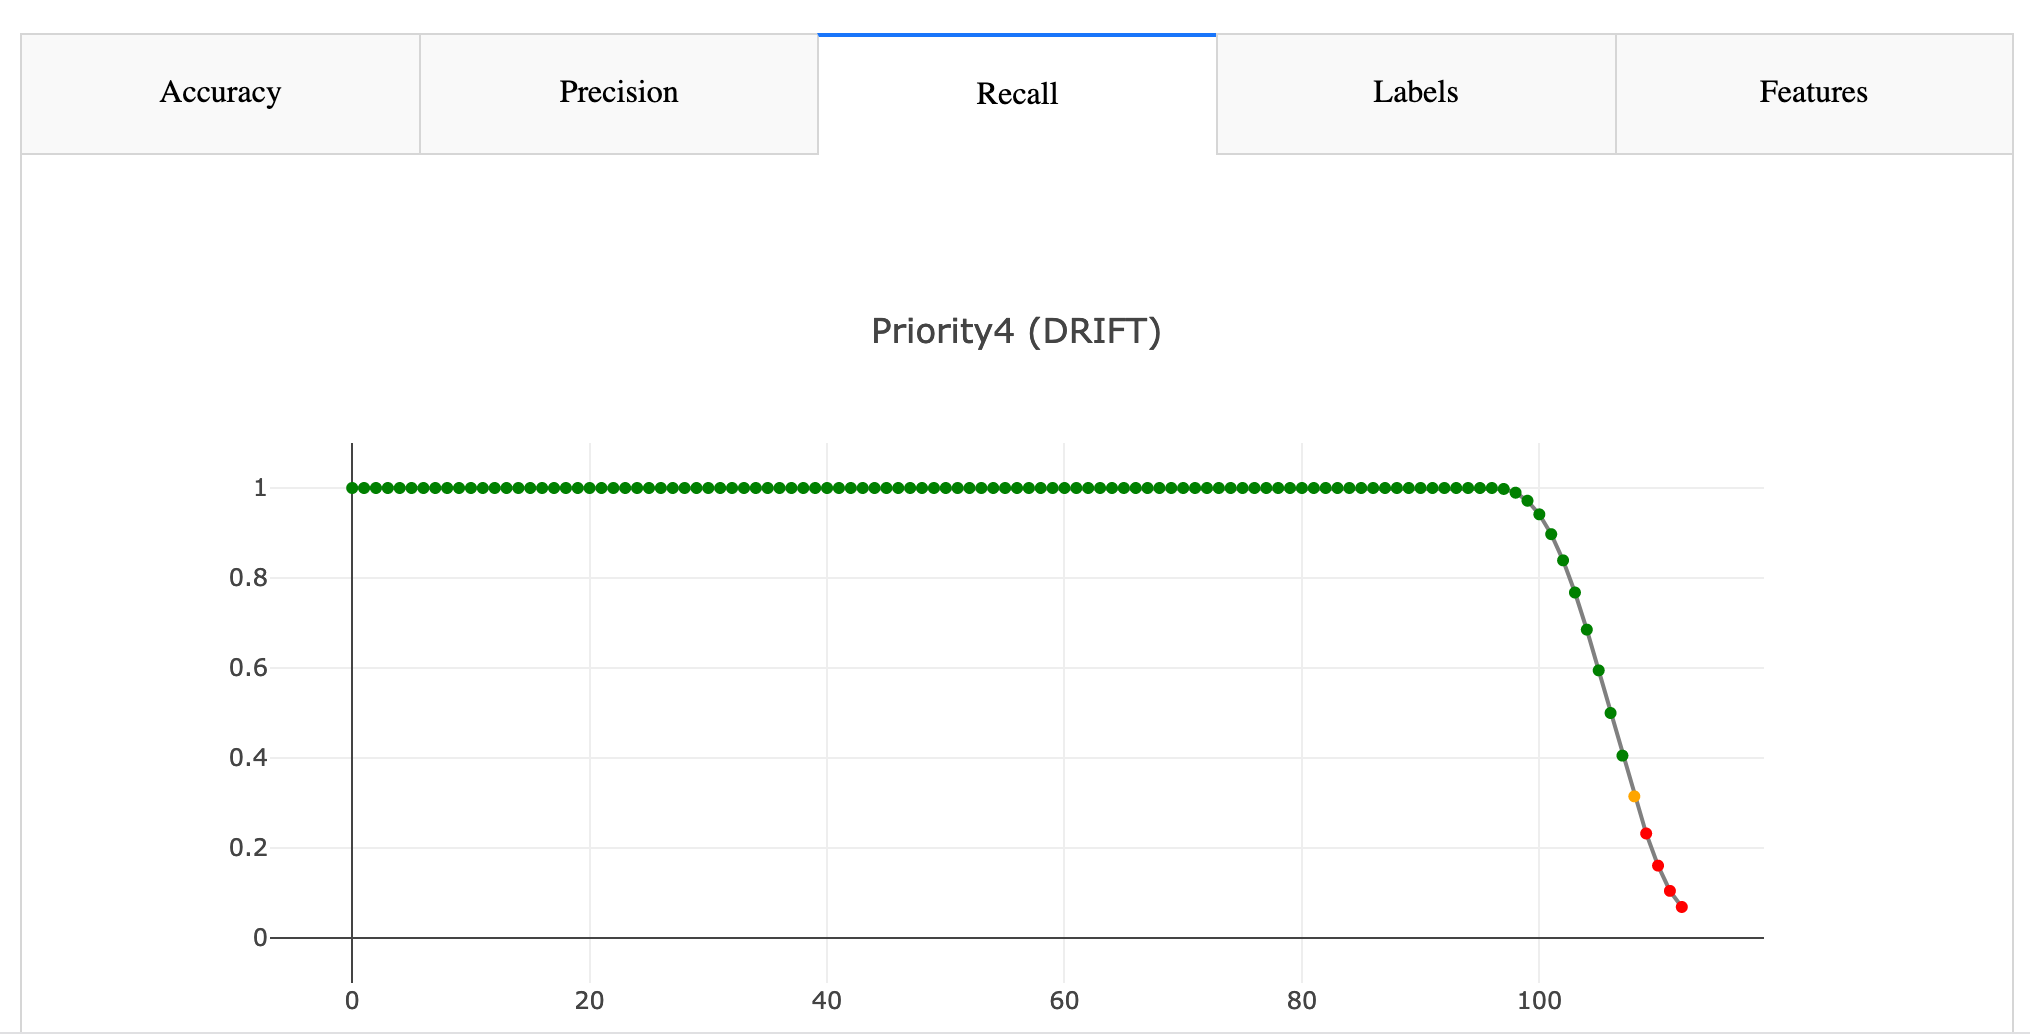
\includegraphics[width=\textwidth]{images/recall_p4.png}
    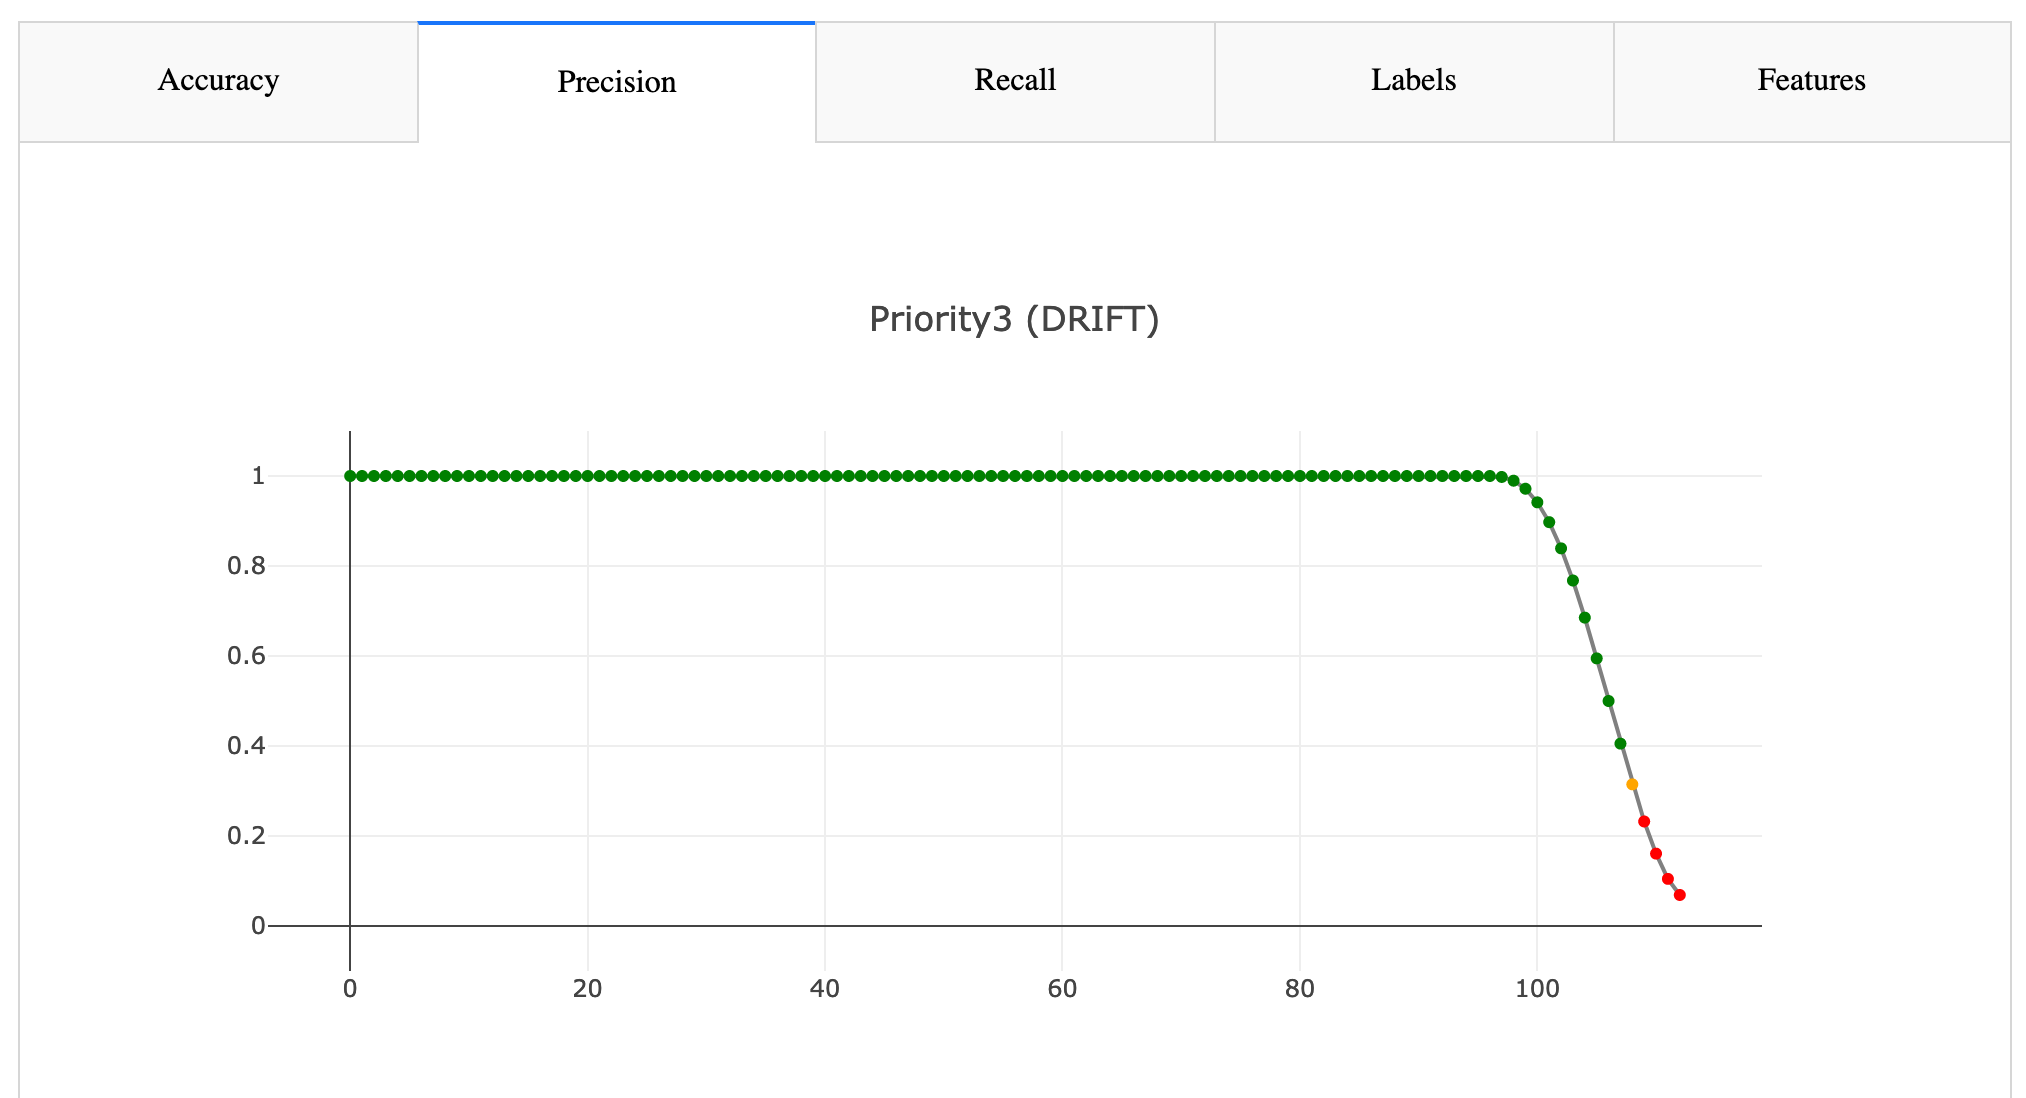
\includegraphics[width=\textwidth]{images/precision_p3.png}
    \caption{Scenario 1: Declining precision for triage priority 3 and declining recall for triage priority 4.}
    \label{fig:scenario1}
\end{figure}
 

\subsection{Scenario 2: No Action}

Data scientists get a message saying that feature drift and label drift have both occurred. Looking closer at the feature drift, it appears that there has been an increase in referrals for patients with coronavirus. Because these instances are given priority 4, there has also been an increase in priority 4 labels, hence the label drift. See Figure \ref{fig:scenario2}. The data scientists decide that this is probably correct behaviour, and the model has seen coronavirus referrals before so this is an instance of on-manifold feature drift. 
The data scientists keep an eye on the model to make sure this plays out as expected. Indeed, the performance metrics don't change significantly. Thus no action is taken.

\begin{figure}
    \centering
    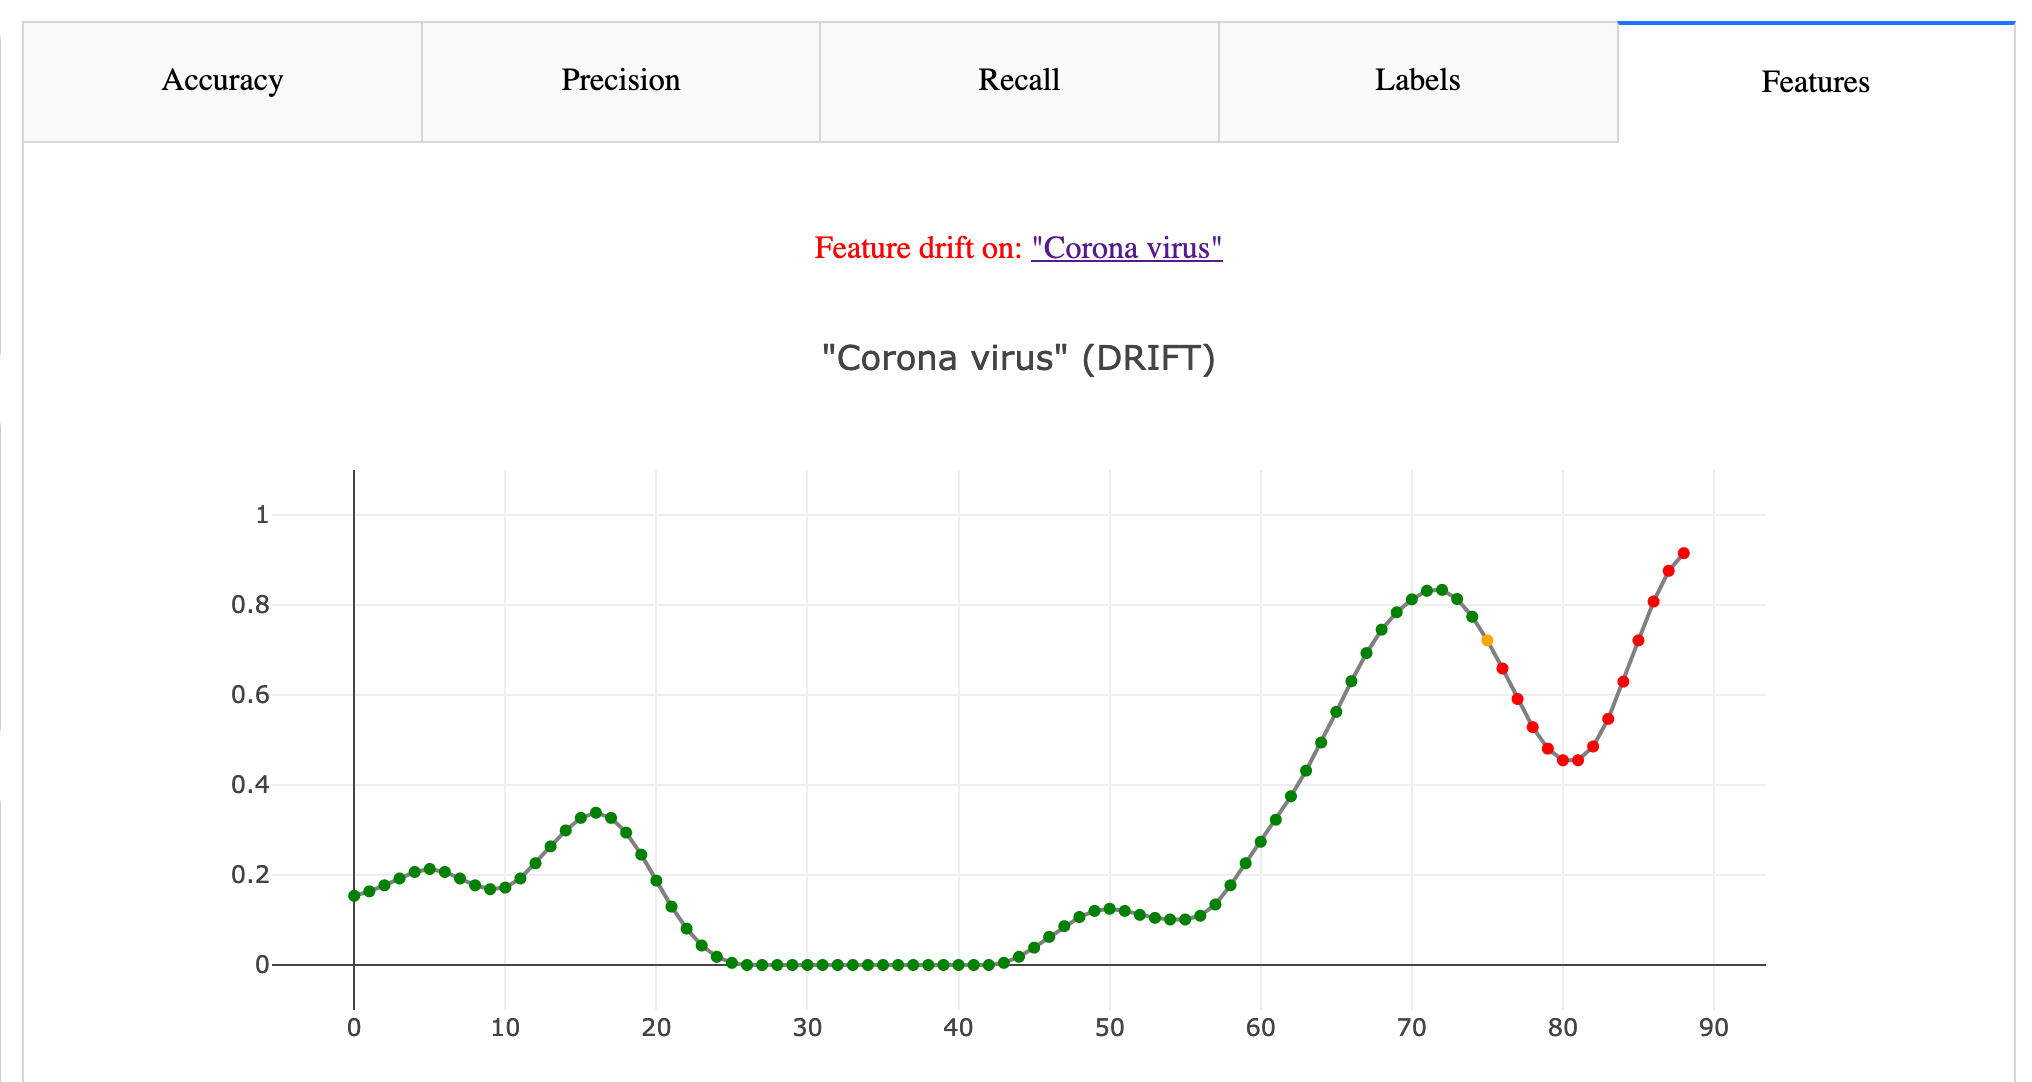
\includegraphics[width=\textwidth]{images/corona_virus.png}
    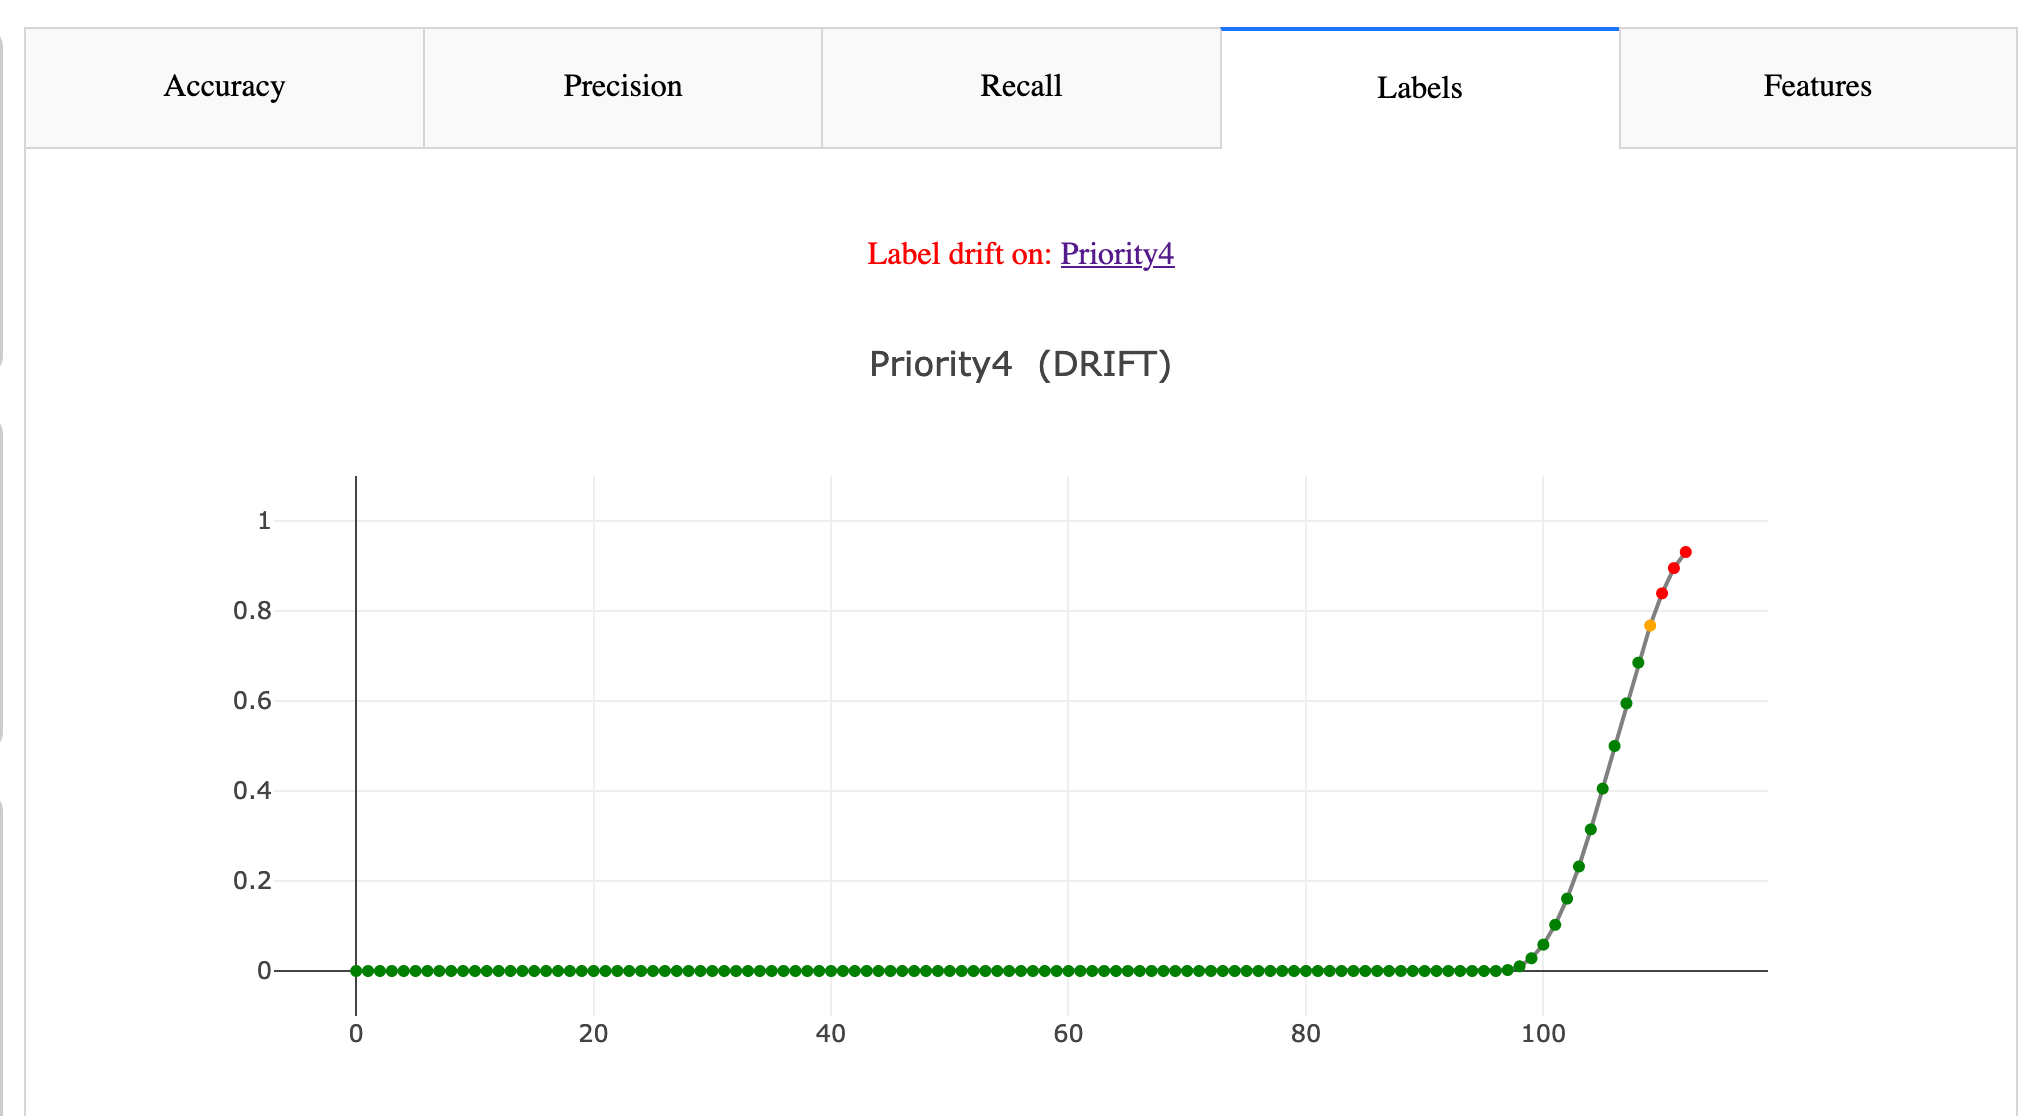
\includegraphics[width=\textwidth]{images/priority4.png}
    \caption{Scenario 2: Increase in the rate of triage priority 4 and increase in the rate of feature ``Corona virus".}
    \label{fig:scenario2}
\end{figure}


\subsection{Scenario 3: Recall}

Data scientists get a message saying that feature drift has occurred. 
Looking closer at the feature drift, it appears that there has been an increase in referrals for patients with coronavirus, as shown in Figure \ref{fig:scenario3}.
Because there were no coronavirus patients in the training data, the data scientists conclude that the model will be unable to make sensible triage predictions for this current wave of patients.
These predictions are therefore clinically unsafe, and so should be withdrawn from the decision support system.
They therefore add a business rule to the priority prediction module stating that if a patient has coronavirus, the model should refrain from making a prediction, and annotate the referral as requiring a clinician to label it.
Once a sufficient dataset of labels for coronavirus patients has accumulated, the model is retrained to handle this new class of patient referral. 

\begin{figure}
    \centering
    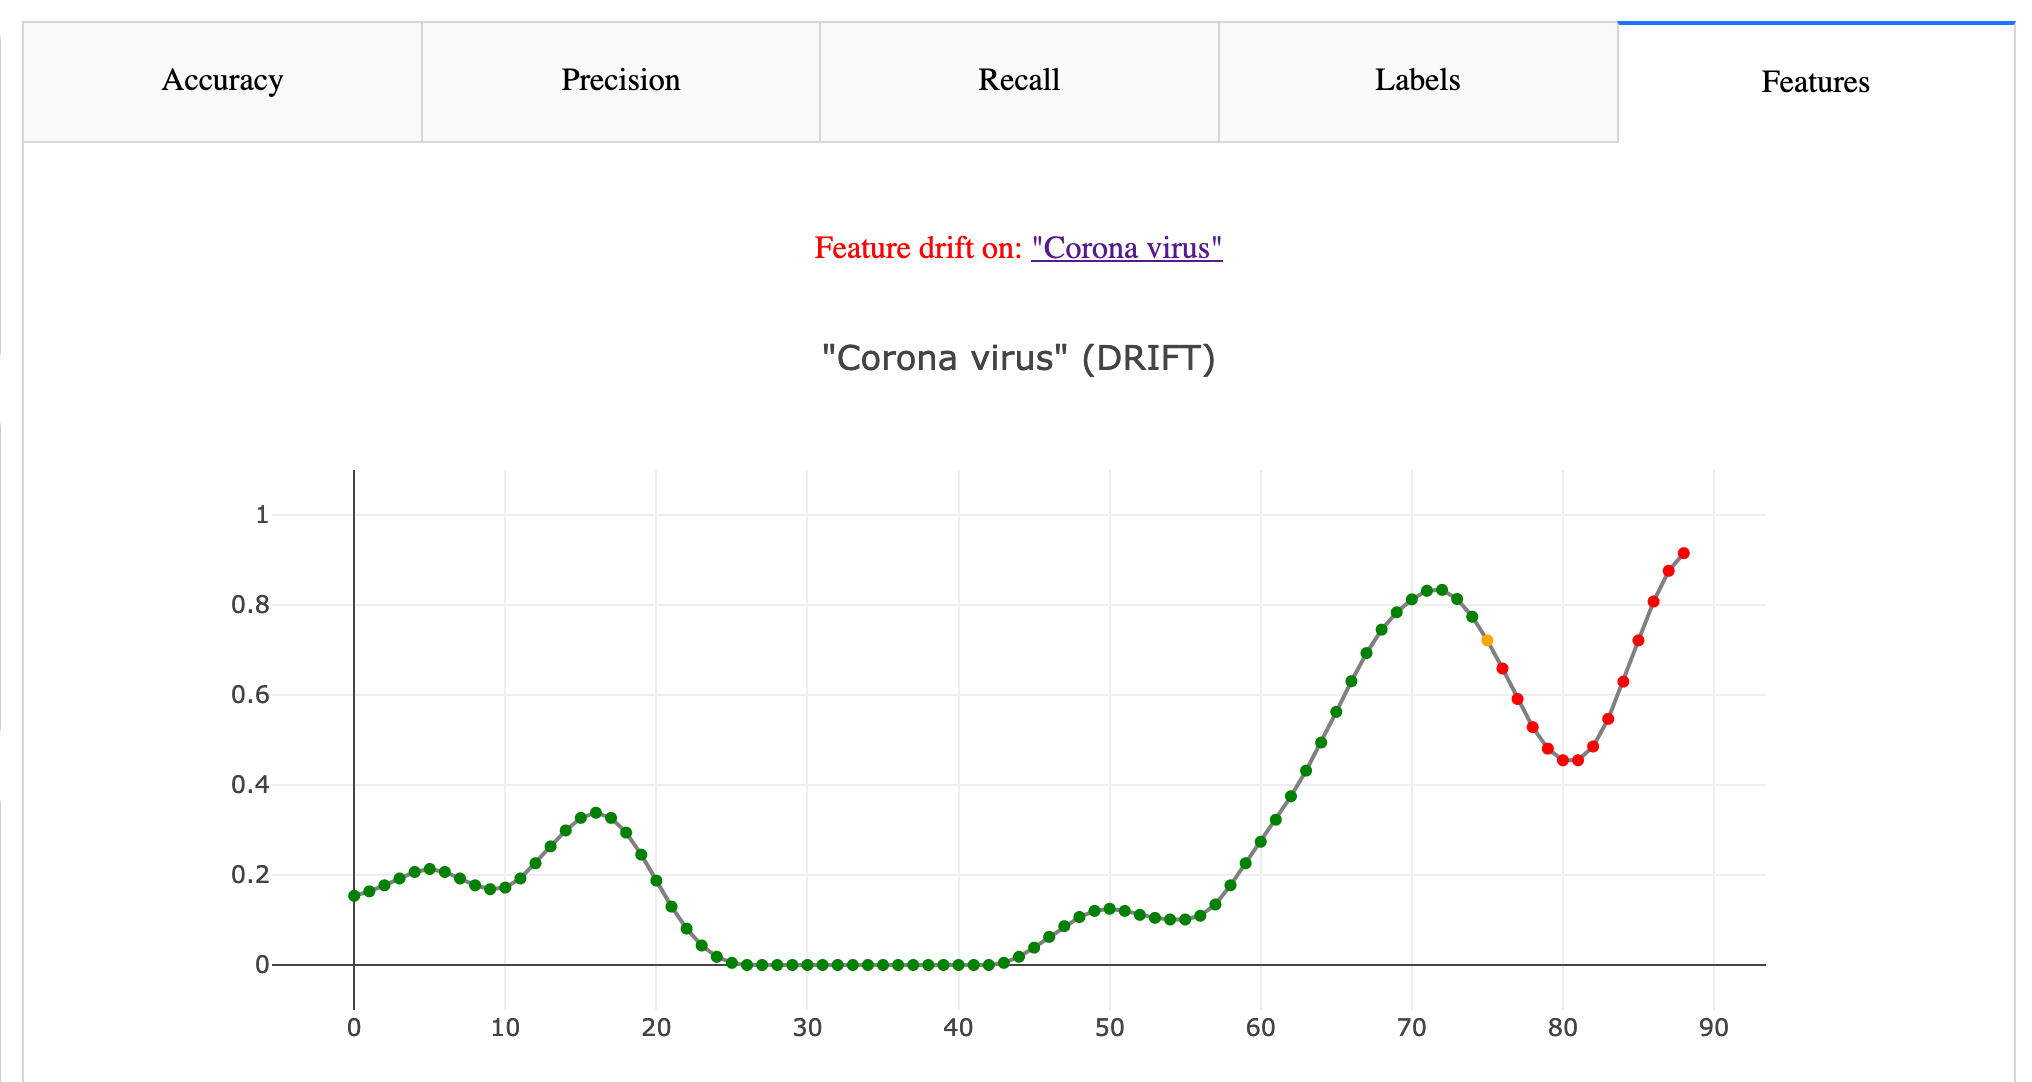
\includegraphics[width=\textwidth]{images/corona_virus.png}
    \caption{Scenario 3: Increase in the rate of feature ``Coronavirus" only.}
    \label{fig:scenario3}
\end{figure}


%-------------------------------------------------------------------
% CONCLUSION
%-------------------------------------------------------------------

\section{Conclusion} \label{mdd:conclusion}

In this chapter we ask ``are existing approaches to concept drift detection suitable for practical data science, and if not how can they be modified to become so?" We argue that there are many implicit or explicit ``axioms" of concept drift detection which will not obtain in practical data science. In particular, we use GP referrals triage as a motivating example for this discussion. We argue for a new operationalisation of concept drift, which we suggest is better suited for practical data science in general, and GP referrals triage in particular. We call an implementation of this operationalisation a multiple drift detector, and explain how to construct such an entity from existing drift detection methods. We also present a graphical interface for a multiple drift detector. We then return to our motivating example of GP referrals triage, and discuss three scenarios in which multiple drift detector would be valuable.

\chapter{Calibrated Drift Detection Method} \label{chapt:CDDM}

In this chapter we introduce calibrated drift detection method (CDDM), a drift detection method which detects increases in the irreducible error rate, rather than the overall error rate. Section \ref{CDDM:motivation} motivates the approach to concept drift detection taken by CDDM. Section \ref{cddm:setting} discusses the setting and notation of CDDM. Section \ref{CDDM:algorithm} provides the actual CDDM algorithm. Section \ref{CDDM:limitations} discusses theoretical and practical limitations of CDDM. Section \ref{CDDM:conclusion} summarises this chapter and discusses future work. 

%-------------------------------------------------------------------
% MOTIVATION
%-------------------------------------------------------------------

\section{Motivation} \label{CDDM:motivation}

Most, if not all, extant drift detectors assume that significant increases in the error rate of the base learner are due to concept drift and require model retraining. For example, Gama et al. \cite{DDM} state 
\begin{displayquote}
    Statistical [sic] theory \cite{statistical_theory} guarantees that while the class distribution of the examples is stationary, the error rate of the learning algorithm ($p_i$) will decrease when $i$ increases. A significant increase in the error of the algorithm, suggest a change in the class distribution, and that the actual decision model is not appropriate.
\end{displayquote}

\noindent However, this assumption is invalid in environments when 1) some labels can be predicted more easily than others, and 2) feature drift occurs. Consider the following (fictional) example from our motivating domain of medical triage:
\begin{displayquote}
    At a coronavirus emergency clinic, patients with coronavirus symptoms are being triaged. Young patients have a low mortality rate from coronavirus so are given low priority. Old patients have a high mortality rate so are given high priority. Middle aged patients, however, may have high or low mortality depending on other factors, so may be given a high, low, or medium priority. 
    
    The learner is easily able to discover the relationship between age and priority, but fails to make use of other features. The model thus has a higher error rate for middle aged patients than young or old patients. If there is an increase in the number of middle aged patients with coronavirus, then the overall error rate of the model will increase.  
    
    A concept drift detector will detect the increase in the error rate and signal that the model requires retraining. However, because the actual relationship between instances and labels has not changed, retraining the model would at best be a waste of time, and at worst result in an inferior model trained on a smaller dataset. 
    
    Conversely, suppose that instead of an increase in the middle aged patients there is a {\it decrease in middle aged patients}. This will reduce the average difficulty of the prediction task, and reduce the error rate of the model. 
    
    Suppose that shortly after this occurs, the clinic decides to change its triage policy for dealing with middle aged patients. Because the model is trained to implement the old policy, its error rate for middle aged patients will further increase, but this increase may be cancelled out by the decrease from the reduced number of middle aged patients. 
    
    Thus, a concept drift detector may fail to notice the real drift which has occurred, and the model will not be retrained despite the change in the decision boundary. This situation may therefore result in a false negative.
\end{displayquote}
This example illustrates that a concept drift detector should not monitor for increases in the error rate of the model {\it per se}. Instead it should monitor for increases in rate of {\it reducible} error due to {\it real} drift which is {\it not} predictable {\it ex ante} from the prediction task becoming more difficult on average. An increase in the {\it irreducible} error due to {\it virtual} drift which {\it is} predictable {\it ex ante} is a confounder. It can cause false negatives and false positives, such that the model may not be retrained when it should be, and may be retrained when it does not need to be.

%-------------------------------------------------------------------
% SETTING
%-------------------------------------------------------------------

\section{Setting} \label{cddm:setting}

Let $y$ be the true label given to some instance $x$, and $\hat{y}$ be the label predicted by the model. Due to noise, stochasticity, or the limited inferential capabilities of the learner, there is some probability that the model will make the wrong prediction. We thus denote
\begin{equation}
q = \Pr(y=\hat{y})
\end{equation}
as the {\bf reliability} of the model, or the probability that the model will make the correct prediction, for the given instance. 

We assume our model makes probabilistic predictions. We can thus talk about the model {\bf confidence} as the probability assigned by the model to its predicted label, denoted
\begin{equation}
\hat{q} = \hat{\Pr}(y=\hat{y}).
\end{equation}
A plot of a model's confidence versus its reliability is called a {\bf reliability diagram} \cite{calibrating}, and is illustrated in Figure \ref{fig:calibration}. 

\newcommand{\calibrationgraph}[7][]{
    % args:
    \draw [thick, <->] (0,1.25) -- (0,0) -- (1.25,0);
    \node [below] at (1.25,0) {$\hat{q}$};
    14
    \node [left] at (0,1.25) {$q$};
    \node [left] at (0,#7) {$q_t$};
    \node [below] at (#6,0) {$\hat{q}_t$};
    \draw (#2,#3) -- (#4,#5);
    \draw [red] (#6,0) -- (#6,#7);
    \draw [red, dashed] (0,#7) -- (#6,#7);
}

\begin{figure}
    \centering
    \begin{tikzpicture}[scale=3]
        \calibrationgraph{0}{0}{1}{1}{0.5}{0.5}
    \end{tikzpicture}
    \caption{Calibration Graph}
    \label{fig:calibration}
\end{figure}

When a model's confidence is equal to its reliability, $q=\hat{q}$, we say that the model is {\bf calibrated} \cite{superforecasting}\cite{scoring_rules}\cite{calibrating}. For example, if a calibrated model makes 10 predictions, and assigns a 0.9 confidence to each of them, then in expectation, one of those predictions will turn out to be incorrect. The reliability diagram in Figure \ref{fig:calibration} is of a calibrated model, as it shows an identity relationship between confidence and reliability.

\newcommand{\calibrationgraphB}[7][]{
    % args:
    \draw [thick, <->] (0,1.25) -- (0,0) -- (1.25,0);
    \node [below] at (1.25,0) {$\hat{q}$};
    14
    \node [left] at (0,1.25) {$q$};
    \node [left] at (0,#7) {$Acc$};
    \node [below] at (#6,0) {$\mathbb{E}[\hat{q}]$};
    \draw (#2,#3) -- (#4,#5);
    \draw [red] (#6,0) -- (#6,#7);
    \draw [red, dashed] (0,#7) -- (#6,#7);
}

\newcommand{\virtualdriftgraph}[3][]{
    \begin{tikzpicture}[scale=3]
        \calibrationgraphB{0}{0}{1}{1}{0.5+#2}{0.5+#2}
        \draw [red, thick, ->] (0.5, #3) -- (0.5+#2*1.5, #3);
    \end{tikzpicture}
}

\begin{figure}
    \centering
    \begin{tikzpicture}[scale=3]
        \calibrationgraphB{0}{0}{1}{1}{0.5}{0.5}
    \end{tikzpicture}
        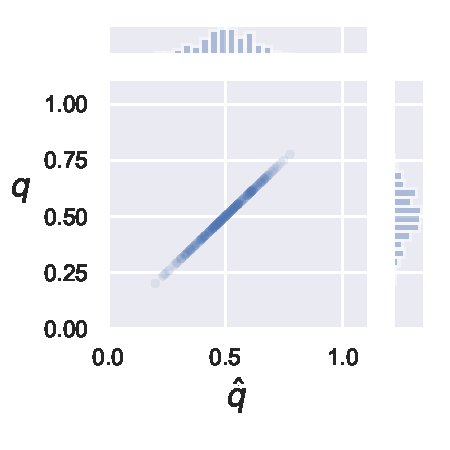
\includegraphics[width=0.3\textwidth]{images/no_drift.pdf}
    \caption{A calibrated model.}
    \label{fig:no_drift}
\end{figure}

When a model is calibrated, we can estimate the accuracy and error rate of the model from its confidence. Figure \ref{fig:no_drift} shows a reliability diagram plus the distribution over confidence values, and thus the distribution over reliability. The accuracy is the expected value of the reliability 
\begin{equation}
    Acc = \mathbb{E}[q]
\end{equation}
and the error rate is one minus the accuracy:
\begin{equation}
    Err = 1 - Acc = \mathbb{E}[q].
\end{equation}
In this manner we may derive an {\it ex ante} estimation of the model's accuracy based on its confidence scores. If the actual {\it ex post} accuracy significantly deviates from this accuracy, then we have evidence that the model is miscalibrated, which we take as evidence of concept drift.

Suppose the average difficulty of the prediction task increases, as described in Section \ref{CDDM:motivation}, and illustrated in Figure \ref{fig:pos_virt}. A calibrated model will decrease in its mean confidence, and our {\it ex  ante} expected error rate will increase. When we observe an {\it ex post} increase in the error rate we will know that this can be attributed to feature drift rather than due to real drift, and so the model should not be retrained. In other words, we have observed an increase in the irreducible error rather than reducible error. We can thus avoid false positive.

\begin{figure}
    \centering
    \virtualdriftgraph{-0.2}{0.125}     
    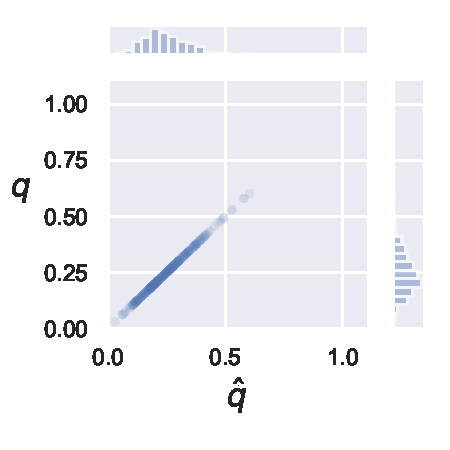
\includegraphics[width=0.3\textwidth]{images/positive_virtual.pdf}
    \label{fig:pos_virt}
    \caption{An increase in irreducible error rate.}
\end{figure}

Conversely, consider the other case described in Section \ref{CDDM:motivation} and illustrated in Figure \ref{fig:co_drift}, where the average difficulty of the prediction task decreases around the same time as real drift occurs. In this case the mean confidence of the model decreases, and so {\it ex ante} error rate decreases. If the {\it ex post} error rate does not decrease, this indicates that concept drift has occurred. In other words, there has been an increase in the reducible error rate, but it has been obscured by a decrease in the irreducible error rate. We can thus detect that the model {\it should} be retrained despite no increase in the overall error rate and thus avoid a false negative.

\begin{figure}
    \centering
    \begin{tikzpicture}[scale=3]
        \calibrationgraphB{0.25}{0}{1}{0.75}{0.75}{0.5}
        \draw [black, thick, ->] (0.9, 0.8) -- (0.9, 0.5);
        \draw [red, thick, ->] (0.6, 0.2) -- (0.85, 0.2);
    \end{tikzpicture}
        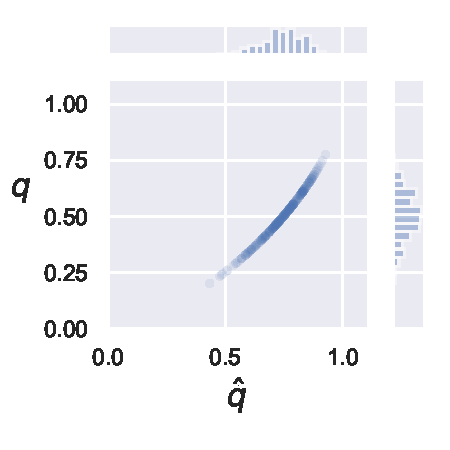
\includegraphics[width=0.3\textwidth]{images/hidden_drift.pdf}
    \caption{A decrease in irreducible error masking an increase in reducible error.}
    \label{fig:co_drift}
\end{figure}

%-------------------------------------------------------------------
% ALGORITHM
%-------------------------------------------------------------------

\section{Algorithm} \label{CDDM:algorithm}

CDDM detects increases in reducible error rather than overall error by monitoring for differences in the {\it ex ante} accuracy and the {\it ex post} accuracy. 

Intuitively, we can consider CDDM to be placing a ``bet" on each prediction. If the model has confidence $\hat{q}$ in its prediction, then it will buy a bet that it is correct for \$$\hat{q}$. If the prediction turns out to be correct, the model will receive a payoff of \$1, otherwise it will receive a payoff of \$0. The payoff is denoted:
\begin{equation}
    \gamma = \begin{cases} 
        1-\hat{q} & \text{if }y=\hat{y} \\ 
        -\hat{q} & \text{if }y\ne\hat{y}
    \end{cases}
\end{equation}
The expected value of the payoff under normal, calibrated conditions is zero:
\begin{align}
	\mathbb{E}[\gamma] &= \Pr(y=\hat{y}) \cdot (1-\hat{q}) - \Pr(y\ne \hat{y}) \cdot \hat{q} \\
	&= q \cdot (1-q) - (1-q) \cdot q \\
	&= 0. \label{eq:expectation}
\end{align}
If we have observed $n$ payoffs, $\gamma_1,\gamma_2,\dots,\gamma_n$, then we can use Hoeffding's inequality \cite{hoeffding} to bound the probability of seeing a large average payoff:
\begin{align}
    \Pr\left(  \left| \frac{1}{n} \sum_{i=1}^n \gamma_i - \mathbb{E}\left[\frac{1}{n} \sum_{i=1}^n \gamma_i\right] \right| \ge k \right)
    &= \Pr\left(  \left| \frac{1}{n} \sum_{i=1}^n \gamma_i \right| \ge k \right) \\
    &\le 2 \exp\left(-\frac{2n^2k^2}{\sum_{i=1}^n(b_i - a_i)^2}\right) \\
    \intertext{Where $a_i$ and $b_i$ are lower and upper bounds on $\gamma_i$, respectively. Because $0\le \hat{q} \le 1$, we have $a_t=-1 \le \id{y_t=\hat{y}_t} - \hat{q}_t \le b_t=1$.}
  &\le \exp\left(-\frac{2n^2k^2}{\sum_{i=1}^n 4}\right) \\
  &\le \exp\left(-\frac{nk^2}{2}\right). \label{eq:hoeffding}
\end{align}
CDDM maintains a sliding window of the most recent $n$ payoff values. Equation \ref{eq:hoeffding} gives a $p$-value for an average payoff across this window at least as extreme as observed. If this value falls below some critical threshold, we may reject the null hypothesis and conclude that the model is miscalibrated. In this case, CDDM will signal that drift has occurred.

Similar to several other drift detectors \cite{DDM}\cite{HDDM}\cite{FLORA}, we use two critical thresholds: $\alpha_{warn}$, a warning threshold, and $\alpha_{drift}$, a drift threshold. When the $p$-value falls below $\alpha_{warn}$, CDDM emits a warning that drift may be occurring, and all new instances are placed in a buffer. When the $p$-value falls below $\alpha_{drift}$, CDDM indicates that concept drift has occurred. The model is then retrained on the instances in the buffer. The full pseudocode is given in Algorithm \ref{alg:cddm_basic}.

\begin{algorithm}
    \caption{CDDM algorithm}
    \label{alg:cddm_basic}
    \begin{algorithmic}
    \Require Warning threshold $\alpha_{warn}$
    \Require Drift threshold $\alpha_{drift}$
    \Require Window size $N$
    \State Window $\gets$ []
    \State {\tt status} $\gets$ {\tt normal}
	\For {$y_t, \hat{q}_t, \hat{y}_t$ in the data stream}
        \State $\gamma_t \gets \id{y=\hat{y}} - \hat{q}$
        \State Window $\gets \{\gamma_t\} \cup$ Window
        \State $n =$ Window.length
        \If {$n > N$}
            \State Window.pop()
        \EndIf
        \State $k \gets \left| \text{Window.mean} \right|$
        \State $p \gets 2\exp\left(-\frac{nk^2}{2}\right)$
        \If {$p \leq \alpha_{drift}$}
            \State {\tt status} $\gets$ {\tt drift}
        \ElsIf {$p_{min} \leq \alpha_{warn}$}
            \State {\tt status} $\gets$ {\tt warn}
        \EndIf
    \EndFor
    \end{algorithmic}
\end{algorithm}

%-------------------------------------------------------------------
% LIMITATIONS
%-------------------------------------------------------------------

\section{Limitations} \label{CDDM:limitations}

CDDM suffers from two major limitations. The first is that CDDM requires learners to be calibrated, but most machine learning algorithms are not calibrated out of the box. The second is that small deviations from calibration will not be detectable by CDDM.

\subsection{Calibration}

CDDM requires the base learner to be calibrated. In fact few machine learning models are calibrated out of the box, and require post-hoc transformations of  their probabilistic predictions to become calibrated.

Some models are ``overconfident", meaning that the model's confidence tends to exceed its reliability, $\hat{q}>q$. Some deep learning models such as LeNet \cite{lenet} suffer from overconfidence \cite{nn_calibration}.

Conversely, some models are ``underconfident", meaning that the model's reliability tends to exceed its confidence, $\hat{q}<q$. Some deep learning models such as ResNet \cite{resnet} suffer from underconfidence \cite{nn_calibration}.  

Other models tend to ``extremism", meaning that they are underconfident for confidences close to 0, and overconfident for confidences close to 1.  Extremist models can be considered as pushing $\hat{q}$ values towards 0 and 1 with respect to $q$ values. Maximum margin methods such as boosted trees and boosted stumps are prone to extremism \cite{calibrating}.

The opposite behaviour to extremism is ``moderatism", meaning the model is underconfident for confidence values close to 1 and overconfident for confidence values close to 0. Thus, $\hat{q}$ values are pushed {\it away from} 0 and 1 with respect to $q$ values. Na\"{i}ve Bayes models are prone to moderatism due to making unrealistic independence assumptions \cite{calibrating}. 

The terms ``overconfident" and ``underconfident" are standard in the prediction literature \cite{superforecasting}. ``Extremism" and ``moderatism" are our own terminology. These behaviours are illustrated with reliability diagrams in Figure \ref{fig:calib_drift_types}. 

\begin{figure}%[t!]
    \centering
    \subfigure[Underconfidence]{
        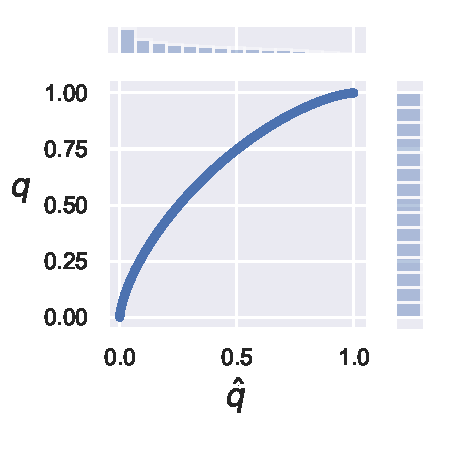
\includegraphics[width=0.45\textwidth]{images/overconfident.pdf}
    }
    \subfigure[Overconfidence]{
        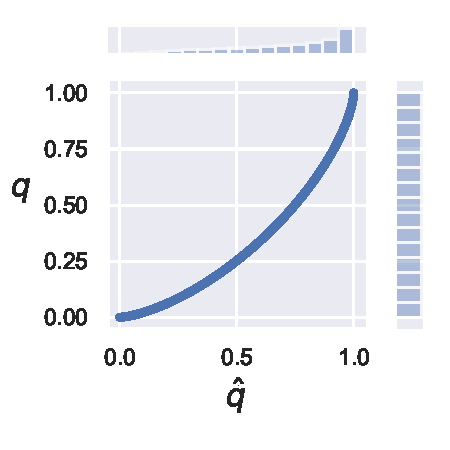
\includegraphics[width=0.45\textwidth]{images/underconfident.pdf}
    }
    \subfigure[Extremism]{
        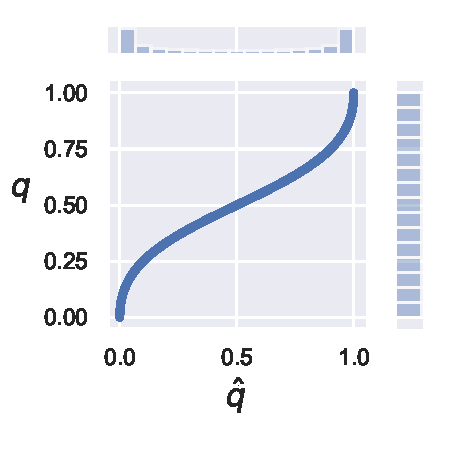
\includegraphics[width=0.45\textwidth]{images/extremist.pdf}
    }
    \subfigure[Moderatism]{
        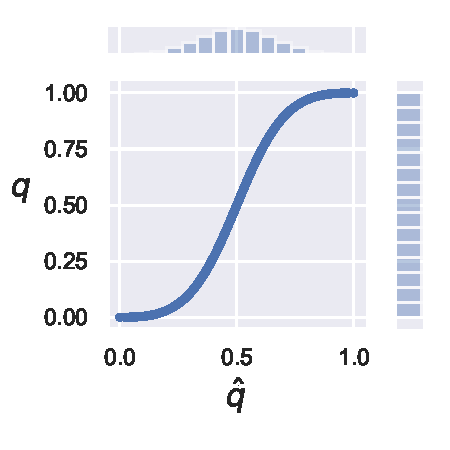
\includegraphics[width=0.45\textwidth]{images/moderate.pdf}
    }
    \caption{Reliability diagrams for a common model behaviours.}
    \label{fig:calib_drift_types}
\end{figure}

Models are often not calibrated because they are designed to optimise some metric other than calibration, such as accuracy. However, even in cases where models {\it are} optimised for calibration, miscalibration can still occur. For example, minimising cross entropy is a standard optimisation objective in deep learning \cite{deep_learning}. This is a proper scoring rule \cite{scoring_rules}, so this optimisation encourages both calibration and accuracy. However, many deep learning models still fail to calibrate \cite{nn_calibration}. This may be due to lack of robustness against dataset shift \cite{dataset_drift}, or overfitting the training data \cite{nn_calibration}.

A model which is not calibrated can be remedied by applying a post-processing function to a model's probabilistic predictions. This function is called a {\bf calibration map} \cite{calibrating}. A variety of methods for generating calibration maps have been developed. Some of the major methods are given below.

Logistic calibration - also called {\bf Platt scaling} \cite{platt} fits a sigmoid function, given by
\begin{equation}
	q = \frac{1}{1 + \exp(a\hat{q} + b)}
\end{equation}
to model probabilities. The parameters $a$ and $b$ are fitted using maximum likelihood estimation on a calibration set. Logistic calibration tends towards exactly correct calibration when the model's confidence values are normally distributed \cite{beyond_sigmoids}. 

Isotonic calibration is a non-parametric type of calibration map \cite{isotonic_calibration}. It is therefore more flexible than logistic calibration, but more prone to overfitting. The only assumption isotonic regression makes about the reliability diagram is that it is isotonic, that is, it is monotonically increasing. 

Beta calibration is a generalisation of sigmoid calibration \cite{beyond_sigmoids}. A beta calibration map takes the form
\begin{equation}
	q = \frac{1}{1 + 1/\left(e^c\frac{\hat{q}^a}{(1-\hat{p})^b}\right) }
\end{equation}
where $a,b\ge 0$ so that the map is monotonically non-decreasing. This map can be fitted as easily as a logistic map \cite{beyond_sigmoids}. Beta calibration is intended to overcome some of the drawbacks of logistic calibration, such as distortions for many classifiers including Naive Bayes and Adaboost. Beta calibration tends towards exactly correct calibration when the model's confidence values are beta distributed. Experiments have found beta calibration to be superior to logistic calibration for Na\"{i}ve Bayes, Adaboost, Random Forests, logistic regression, support vector machines, and multilayer perceptrons \cite{beyond_sigmoids}. 

Other calibration map methods include histogram binning \cite{histogram_calibration}, Bayesian binning into quantile (BBQ) \cite{bbq_binning}, matrix and vector scaling \cite{nn_calibration}, and temperature scaling \cite{nn_calibration}\cite{temperature_scaling}.

\subsection{Small Deviations from Calibration}

CDDM cannot detect small deviations from calibration. Suppose the base learner has been calibrated up to time $t-n$, and from $t-n$ to $t$ it has been slightly overconfident (or underconfident). Specifically,
\begin{equation}
    \delta_i = \begin{cases}
        0 & 0 \le i < t-n \\ 
        \left| \hat{q}_i - q_i \right| & t-n \le i < t
    \end{cases}
\end{equation}
Given a window size $N$, the miscalibration will be on the cusp of detectability from CDDM when the $p$-value given by equation Equation \ref{eq:hoeffding} is equal to the drift detection threshold $\epsilon$: 
\begin{equation}
    \epsilon = \exp\left(-\frac{n^2\delta^2}{2N}\right).
\end{equation}
Solving for $\delta$ gives the minimum overconfidence value which can be detected within $n$ time steps for a given drift threshold and window size:
\begin{align}
    \delta &= \sqrt{-\frac{2N}{n^2}\ln\left(\frac{\epsilon}{N}\right)}.
\end{align}
This relationship is plotted for a range of window sizes with drift threshold 0.01 in Figure \ref{fig:cddm_window_size}. In this plot we can see that, for example, an overconfidence of $\delta=0.4$ can be detected within 250 time steps for a window size of 2000.

\begin{figure}
    \centering
    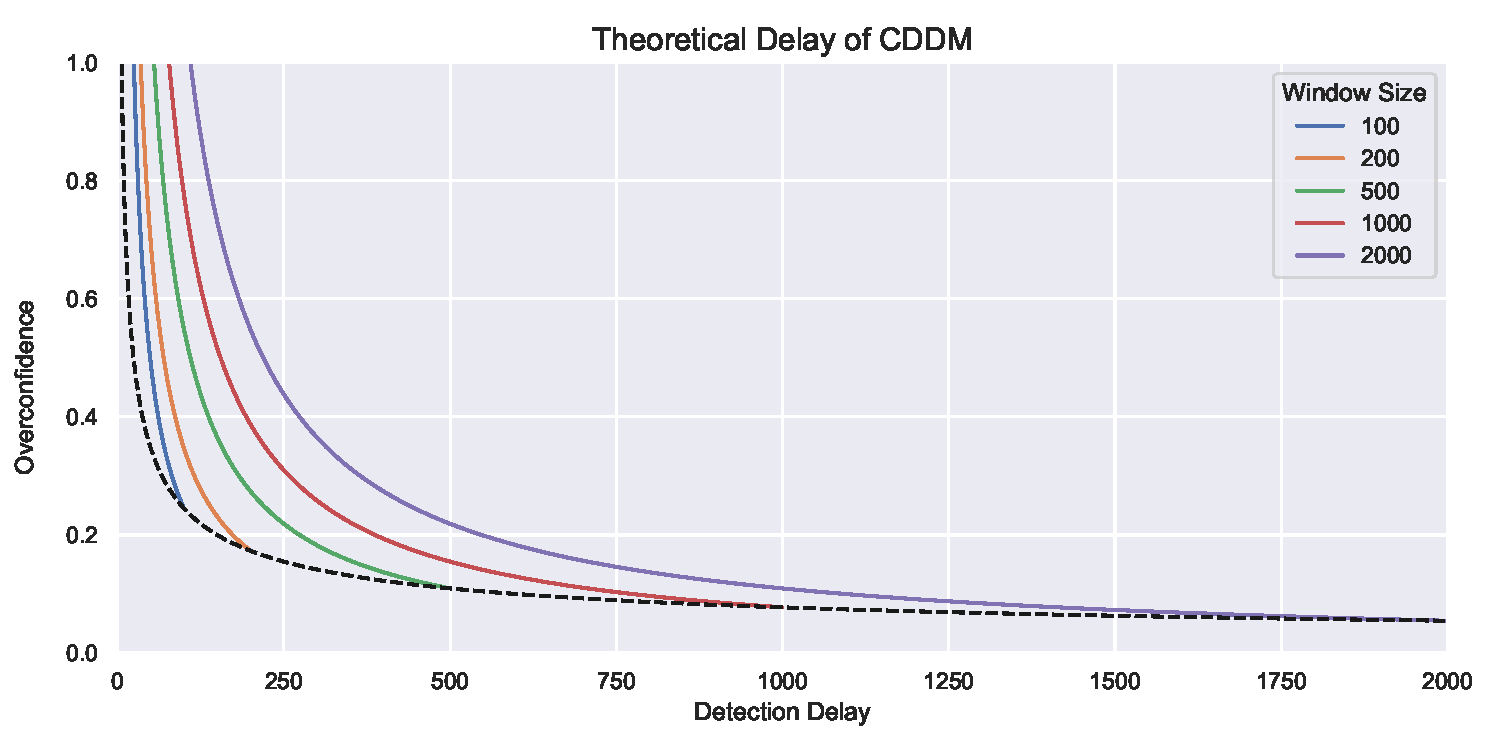
\includegraphics[width=\textwidth]{images/cddm_window_size.pdf}
    \caption{Detection delay versus overconfidence magnitude for CDDM.}
    \label{fig:cddm_window_size}
\end{figure}

The smallest overconfidence value which can possibly be detected by CDDM is found by setting $n=N$. That is, it is only detectable when the entire window has filled up with the miscalibrated payoffs. The range of detectable miscalibrations is thus given by 
\begin{equation}
    1 \ge \delta \ge \sqrt{-\frac{2}{N}\ln\left(\frac{\epsilon}{N}\right)}. \label{eq:window_size}
\end{equation}
The dashed line in Figure \ref{fig:cddm_window_size} indicates this lower bound on detectable miscalibration. This shows that, for example, a miscalibration of magnitude $\delta=0.1$ will be undetectable with a window size of $N=200$.

%-------------------------------------------------------------------
% CONCLUSION
%-------------------------------------------------------------------

\section{Conclusion} \label{CDDM:conclusion}

In this chapter we introduced calibrated drift detection method (CDDM). We argued that a drift detector should detect increases in the reducible error rate rather than the overall error rate, so as to avoid unnecessary retraining. CDDM takes this approach to concept drift detection by detecting when a model becomes miscalibrated. However, CDDM still has some significant limitations. Theoretically, CDDM can only detect mean overconfidence below a certain level determined by the window length. Practically, CDDM assumes that a learner is initially calibrated, whereas most models require prediction post-processing to achieve calibration.

A promising direction for future work would be building a calibration map online, and detecting when this calibration map changes, rather than assuming the learner is calibrated in the first place.
\chapter{Bayesian Concept Drift Detection} \label{chapt:BDD}

In this chapter we explore Bayesian approaches to concept drift detection. Section \ref{BDD:motivation} motivates a Bayesian approach to concept drift detection. Section \ref{BDD:bddm} introduces Bayesian drift detection method (BDDM), an exact algorithm for computing posteriors probabilities of concept drift. Section \ref{BDD:BWAF} introduces Bayes with adaptive forgetfulness, an efficient method for approximating posterior probabilities of concept drift. Section \ref{BDD:conclusion} summarises this chapter and discusses future work.

%-------------------------------------------------------------------
% MOTIVATION
%-------------------------------------------------------------------

\section{Motivation} \label{BDD:motivation}

In this chapter we consider methods for deriving a posterior probability distribution over concept drift locations, and of the current error rate of the model. We claim that such a derivation is valuable for many practical data science applications where a human is in the loop and there are strict requirements on performance. As illustration, we return to our motivating example of GP referrals triage. The details of this description are fictional.
\begin{displayquote}
    A model has been trained to predict triage labels for GP referrals documents. A drift detector is has been installed to detect when the error rate of the model increases, at which point it will alert a data scientist that the model requires retraining.   
    
    Suppose the data scientist receives an alert that the error rate of the model has increased. The data scientist now has to decide 1) whether the model really requires retraining, and if so 2) how far back in time should the new training data extend so that the new model is trained only on post-drift instances.
    
    The model is required to have an error rate of at most 5\%, or it is not considered fit for purpose. The cost of retraining the model is \$500, as it requires the data scientist to spend several days on site collecting data, and retraining the new model, validating the new model, and deploying the new model. The cost of keeping a model which is not fit for purpose deployed is estimated at \$5000 due to errors in the triage support  leading to inefficient allocation of medical staff. If $\Pr(err>0.05)$ is the probability that the error rate is greater than 5\%, then it is worthwhile retraining the model as long as 
    \begin{equation}
        \Pr(err>0.05) \times \$5000 > \left( 1-\Pr(err>0.05) \right) \times \$500.
    \end{equation}
    This illustrates that it is not only important for the data scientist to know that the error rate has probably increased, but to also have a probability distribution over {\it how much} it has increased. 
    
    If the data scientist has access to a posterior probability distribution over possible error rates at the current time, as in Figure \ref{fig:posterior_rates}, then they can make a more informed decision about whether the model requires retraining or not.   
    
    Let us suppose the data scientist decides that the model {\it does} require retraining. They must now decide which data to use to retrain the model. Other things being equal, the data scientist would like to use more data rather than less so that the model will generalise better. However, the less recent the data, the more likely it is to have become outdated by the concept drift.
    
    Again, the data scientist would be assisted by a posterior probability mass function, this time over possible times at which the concept drift occurred, as in Figure \ref{fig:bayes_pdf}. This gives the posterior probability of a concept drift having occurred at each of the time steps. For time step $t$, this probability is denoted $\Pr(d=t)$. 
    
    Figure \ref{fig:bayes_pdf} also gives a cumulative mass function. This illustrates the posterior probability of concept drift having occurred {\it by} each time step. This is denoted as $\Pr(d\le t)$. 
    
    With these posterior distributions, the data scientist can decide which instances to use in the training data to maximise expected utility. 
    
    For example, suppose the cost of including outdated instances is equal to the cost of not including relevant instances in the training data. In this case the data scientist will want to include all instances after the time at which the probability of concept drift having occurred was 50\%. Thus in Figure \ref{fig:bayes_pdf}, the model would be retrained using instances which became available after $t=40$.
\end{displayquote}

\newcommand*\GnuplotDefs{
    % set number of samples
    % source: https://tex.stackexchange.com/questions/368146/how-to-draw-pdf-curves-for-beta-distribution
    set samples 123;
    %
    % define beta distribution function
    % (copied from <http://gnuplot.sourceforge.net/demo/prob.5.gnu>)
    Binv(p,q)=exp(lgamma(p+q)-lgamma(p)-lgamma(q));
    beta(x,p,q)=p<=0||q<=0?1/0:x<0||x>1?0.0:Binv(p,q)*x**(p-1.0)*(1.0-x)**(q-1.0);
}

\newcommand{\bwafFig}[8]{
    % args:
    % - a, b of anterograde distribution
    % - a, b of retrograde distribution
    % - x, y of "Anterograde" label
    % - x, y of "Retrograde" label
    \begin{tikzpicture}
        \pgfmathsetmacro{\xmin}{0}
        \pgfmathsetmacro{\xmax}{1}
        \begin{axis}[
            xmin=\xmin,
            xmax=\xmax,
            ymin=-0.01,
            ymax=11,
            xlabel=Error rate $q$,
            ylabel=$\Pr(q)$,
            axis line style={->},
            no markers,
        ]
            \addplot gnuplot [raw gnuplot] {
                % first call all the "common" definitions
                \GnuplotDefs
                plot [x=\xmin:\xmax] beta(x,#1,#2);
            };
            \addplot gnuplot [raw gnuplot] {
                \GnuplotDefs
                plot [x=\xmin:\xmax] beta(x,#3,#4);
            };
            \node [color=blue, right] at (#5,#6) {Anterograde};
            \node [color=red, right] at (#7,#8) {Retrograde};
        \end{axis}
    \end{tikzpicture}
}

\begin{figure}
    \centering
    % \bwafFig{10}{40}{14}{20}{25}{600}{50}{300}
    \begin{tikzpicture}
        % define macros which are needed for the axis limits as well as for
        % setting the domain of calculation
        \pgfmathsetmacro{\xmin}{0}
        \pgfmathsetmacro{\xmax}{1}
        \begin{axis}[
            xmin=\xmin,
            xmax=\xmax,
            ymin=-0.01,
            xlabel=Error rate $q$,
            ylabel=$\Pr(q)$,
            axis line style={->},
            no markers,
        ]
            \addplot gnuplot [raw gnuplot] {
                % first call all the "common" definitions
                \GnuplotDefs
                plot [x=\xmin:\xmax] beta(x,10,40);
            };
            \addplot gnuplot [raw gnuplot] {
                \GnuplotDefs
                plot [x=\xmin:\xmax] beta(x,14,20);
            };
            \node [color=blue, right] at (25,600) {Original};
            \node [color=red, right] at (50,300) {Current};
        \end{axis}
    \end{tikzpicture}
    % 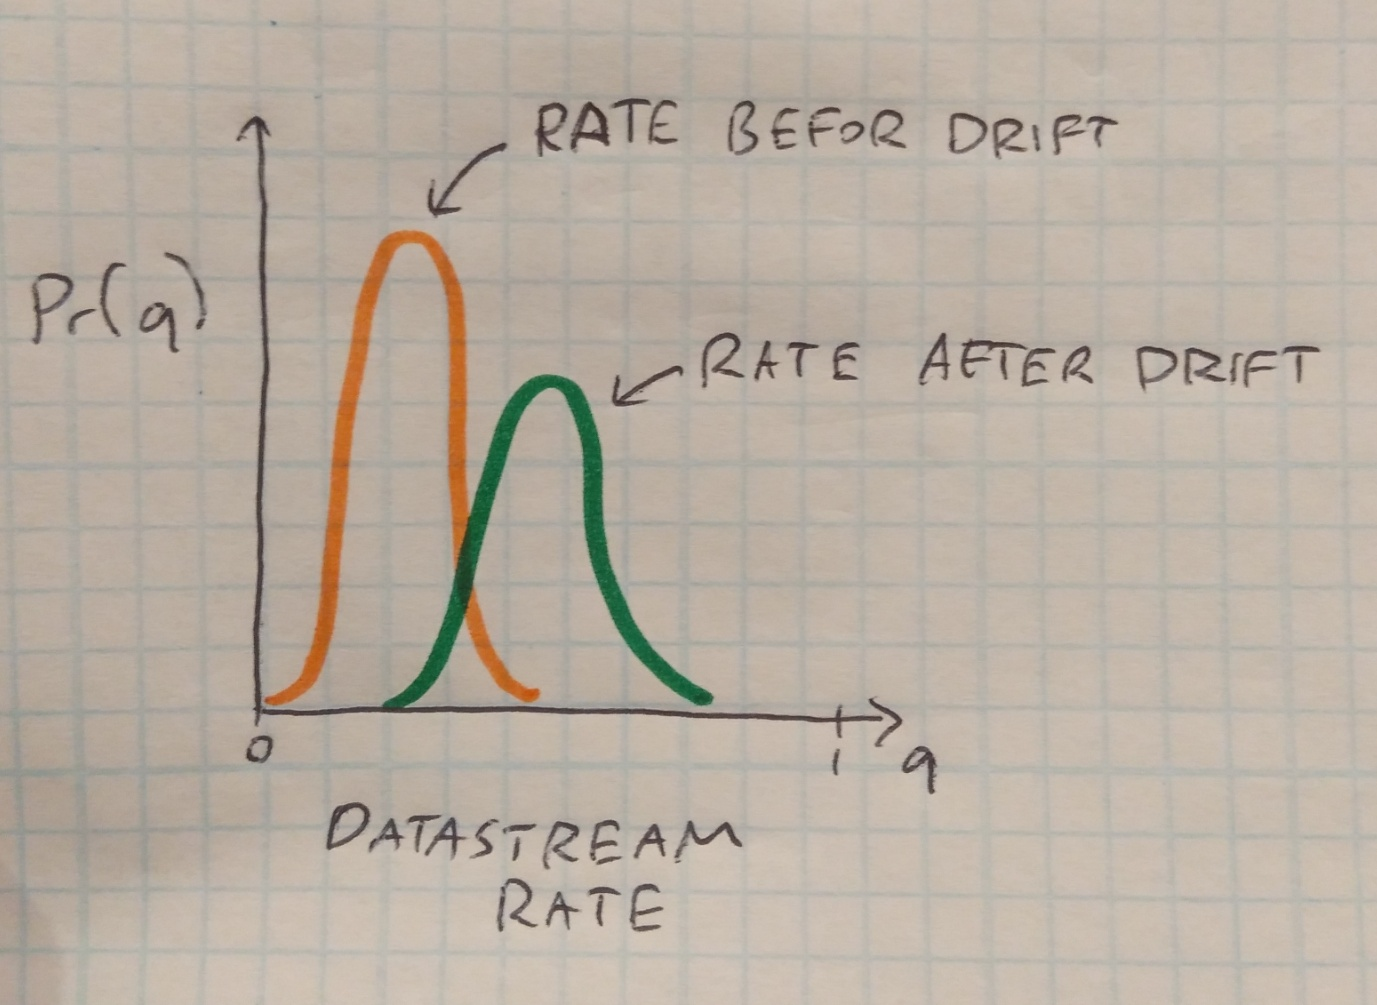
\includegraphics[width=.5\columnwidth]{images/posterior_rates.jpg}
    \caption{Posterior distribution over the original and current error rates of the model when concept drift has occurred.}
    \label{fig:posterior_rates}
\end{figure}



\pgfmathdeclarefunction{gauss}{2}{%
  \pgfmathparse{1/(#2*sqrt(2*pi))*exp(-((x-#1)^2)/(2*#2^2))}%
}
\def\cdf(#1)(#2)(#3){0.5*(1+(erf((#1-#2)/(#3*sqrt(2)))))}%
% to be used: \cdf(x)(mean)(variance)

\begin{figure}
    \centering
    \subfigure[Probability mass function]{
        \begin{tikzpicture}
            % pdf
            \begin{axis}[
                xmin=0,
                xmax=100,
                ymin=0,
                no markers,
                ylabel={$\Pr(d=t)$},
                xlabel=$t$,
                domain=0:100, 
                samples=100,
                width=0.6\textwidth,
                height=0.3\textwidth
            ]
                \addplot {gauss(40,10)};
            \end{axis}
        \end{tikzpicture}
    }
    \subfigure[Cumulative mass function]{
        \begin{tikzpicture}
            % cdf
            \begin{axis}[
                xmin=0,
                xmax=100,
                ymin=0,
                no markers,
                ylabel={$\Pr(d\le t)$},
                xlabel=$t$,
                domain=0:100, 
                samples=100,
                width=0.6\textwidth,
                height=0.3\textwidth,
            ]
                \addplot[smooth,red] gnuplot{\cdf(x)(40)(10)};
            \end{axis}
        \end{tikzpicture}
    }
    \caption{Probability mass function and cumulative mass function over times at which a concept drift may have occurred.}
    \label{fig:bayes_pdf}
\end{figure}

%-------------------------------------------------------------------
% BDDM
%-------------------------------------------------------------------

\section{Bayesian Drift Detection Method} \label{BDD:bddm}

In this section we introduce the Bayesian drift detection method (BDDM). BDDM precisely computes posterior distributions over drift points, as well as the error rates at the start and end of the data stream. It is therefore more precise than other drift detectors, but at the cost of having $O(t^2)$ time complexity and $O(t)$ space complexity. We also present a windowed version which is linear in time and constant in space.

\subsection{Setting}

We pose the problem of computing a posterior over drift points as follows. Given a Bernoulli time series 
\begin{equation}
    Z=z_0,z_1,\dots,z_t
\end{equation}
we would like to compute the probabilities that the rate of the series changed at each time step, as well as the probability no change occurred. The time series in question is the series of residuals of the model. A change in the rate of this series indicates that the error rate has changed which indicates drift.

We denote the probability that a drift occurred at time step $i$ as $\Pr(d=i)$. Specifically, $\Pr(d=i)$ is the prior probability of drift having occurred at time step $i$. The posterior probability is the probability of drift conditioned on the observed time series, denoted $\Pr(d=i|Z)$. For convenience, we denote the probability that no drift has occurred as $\Pr(d=0)$.


We can express the posterior probability of drift at a given time step using Bayes' rule:
\begin{align}
  \Pr(d=i|Z) &= \frac{\Pr(Z|d=i)}{\Pr(Z)}\Pr(d=i) \\
  &= \frac{\Pr(Z|d=i)}{\sum_{j=0}^t\Pr(Z|d=j)\Pr(d=j)}\Pr(d=i) \label{eq:posterior}
\end{align}
For convenience, we will denote the joint probability of a given sequence with a given drift point as
\begin{align}
  P_i &= \Pr(Z, d=i) \\
  &= \Pr(Z|d=i)\Pr(d=i).
\end{align}
The posterior probability that drift has occurred is given by
\begin{align}
  \Pr(d=0|Z) = \frac{\sum_{i=1}^t P_i}{\sum_{i=0}^t P_i}.
\end{align}

\subsection{Priors}

We require a method for setting unitary priors on possible drift points.
\begin{equation}
  \sum_{i=0}^t \Pr(d=i) = 1
\end{equation}
We propose two systems of priors for BDDM, one for evenly spaced time series and one for unevenly spaced time series. Our motivating example of GP referrals triage is an example of an unevenly spaced time series as GP referral documents or clinician labels can arrive at any time.

A natural prior for evenly spaced time series is a geometric distribution \cite{fearnhead}\cite{BCMC}. We suppose that there is a constant rate of concept drift, and that drift may only occur once. This is like flipping a coin at every time step, and allowing drift to occur upon the first heads.
\begin{equation}
  \Pr(d=i) = \begin{cases}
  (1-\lambda)^t & \text{if }i=0 \\
  (1-\lambda)^{d-1}\lambda & \text{if }i>0
  \end{cases}
\end{equation}
where $\lambda \in [0,1]$ is the drift rate, which is the only parameter of BDDM.

We can generalise this strategy to interval settings by modelling drift as a Poisson process. Again, we have a ``rate" of drift, but now the rate is per unit time, not per index.
\begin{align}
  \Pr(d=\tau_i) &= \begin{cases}
  P[N(\tau_t)=0]& \text{if }i=0 \\
  P[N(\tau_{i-1})=0]P[N(\tau_i)>0] & \text{if }i>0
  \end{cases} \\
  &= \begin{cases}
  e^{-\lambda\tau_t} & \text{if }i=0 \\
  e^{-\lambda \tau_{i-1}}\left(1-e^{-\lambda(\tau_i-\tau_{i-1})}\right) & \text{if }i>0
  \end{cases} \\
  &= \begin{cases}
  e^{-\lambda\tau_t} & \text{if }i=0 \\
  e^{-\lambda \tau_{i-1}} - e^{-\lambda \tau_i} & \text{if }i>0 \label{eq:prior}
  \end{cases}
\end{align}
where $\lambda > 0$ is the drift rate and $\tau_i$ is the time between the arrival of the $i$-th value in the data stream and the first value. Note that if the instances are equispaced then this is equivalent to the geometric prior.

\subsection{Likelihoods}

Suppose we have draw a rate from a uniform distribution, and observe a sequence of Bernoulli trials with this rate. The probability of observing a given sequence is given by the beta function with the number of successful trials and the number of unsuccessful trials as arguments.
\begin{align}
  \Pr(Z) &= \int_0^1 x^{\sum_{i=0}^t z_i}(1-x)^{\sum_{i=0}^t 1-z_i} dx \\
  &= B\left(1+\sum_{i=0}^t z_i,1+\sum_{i=0}^t 1-z_i\right) \\
  &= \frac{\left(\sum_{i=0}^t z_i\right)! \left(\sum_{i=0}^t 1-z_i\right)!}{(n+1)!}
\end{align}
where $Z = z_1,z_2,\dots,z_t$ and $B(a,b)$ is the beta function.

If we have a drift point, and the rates for the first and second partition are drawn independently and uniformly, then we have
\begin{align}
  \Pr(Z|d=k) &= \Pr(Z_{0:k-1})\Pr(Z_{k:t}) \\
  &= B\left(1+\sum_{i=0}^{k-1} z_i,1+\sum_{i=0}^{k-1} 1-z_i\right) B\left(1+\sum_{i=k}^t z_i,1+\sum_{i=k}^t 1-z_i\right) \label{eq:likelihood}
\end{align}
where $Z_{a:b}=z_a,z_{a+1},\dots,z_b$.

\subsection{Pseudocode}

By combining the priors from Equation \ref{eq:prior} and likelihoods from Equation \ref{eq:likelihood} into Equation \ref{eq:posterior}, we obtain the posterior probabilities of drift at each time step. We can therefore present the entirety of BDDM in Algorith \ref{alg:bddm}. The algorithm is $O(t^2)$ in time complexity and $O(t)$ in space complexity. We can impose a limit on the resource requirements of BDDM by only considering the most recent $N$ instances as possible drift points. This is achieved by maintaining a sliding window of size $N$, and reduces the time complexity to $O(tN)$ and the space complexity to $O(N)$. The sliding window version of BDDM is given in Algorithm \ref{alg:bddm_win}.

\begin{algorithm}
    \caption{Full BDDM algorithm}
    \label{alg:bddm}
    \begin{algorithmic}
        \Require Drift rate $\lambda$
        \Require Warning threshold $\alpha_{warn}$
        \Require Drift threshold $\alpha_{drift}$
        \For {$t=0,1,2,\dots$}
          \State $c_t \gets (z_t, 1-z_t)$
          \Comment We store $z$ values in dummy vectors.
          \For {$k=0,1,2,\dots,t$}
            \State $P_i \gets B\left(1+\sum_{i=0}^{k-1}c_i\right) B\left(1+\sum_{i=k}^t c_i\right) \Pr(d=\tau_k;\lambda)$
          \EndFor
          \State $P(drift) \gets \frac{\sum_{i=1}^t P_i}{\sum_{i=0}^t P_i}$
          \If {$P(drift)>\alpha_{warn}$}
            \State {\tt status} $\gets$ {\tt warning}
          \ElsIf {$P(drift)>\alpha_{drift}$}
            \State {\tt status} $\gets$ {\tt drift}
          \EndIf
        \EndFor
    \end{algorithmic}
\end{algorithm}

\begin{algorithm}
    \caption{Sliding window BDDM.}
    \label{alg:bddm_win}
    \begin{algorithmic}
        \Require Window size $N$
        \Require Drift rate $\lambda$
        \Require Warning threshold $\alpha_{warn}$
        \Require Drift threshold $\alpha_{drift}$
        \For {$t=0,1,2,\dots$}
          \If {$t<N$}
            \State $c_t \gets (z_t, 1-z_t)$
            \Comment We store $z$ values in dummy vectors.
            \State $\hat{\tau}_t \gets \tau_t$
          \Else
            \State $c_0 \gets c_0 + c_1$
            \State $\hat{\tau}_0 \gets \hat{\tau}_1$
            \For {$i=1,2,\dots,N-2$}
              \State $c_i \gets c_{i+1}$
              \State $\hat{\tau}_i \gets \hat{\tau}_{i+1}$
            \EndFor
            \State $c_{N-1} \gets (z_t, 1-z_t)$
            \State $\hat{\tau}_{N-1} \gets \tau_t$
          \EndIf
          \For {$k=0,1,2,\dots,\min(t,N-1)$}
            \State $P_i \gets B\left(1+\sum_{i=0}^{k-1}c_i\right) B\left(1+\sum_{i=k}^t c_i\right) \Pr(d=\hat{\tau}_k;\lambda)$
            \Comment Where $1$ is a two-dimensional vector.
          \EndFor
          \State $P(drift) \gets \frac{\sum_{i=1}^t P_i}{\sum_{i=0}^t P_i}$
          \If {$P(drift)>\alpha_{warn}$}
            \State {\tt status} $\gets$ {\tt warning}
          \ElsIf {$P(drift)>\alpha_{drift}$}
            \State {\tt status} $\gets$ {\tt drift}
          \EndIf
        \EndFor
    \end{algorithmic}
\end{algorithm}

\subsection{Comparison with other Drift Detectors}

BDDM is closely related, but distinct, from other Bayesian approaches to concept drift detection and change point detection. The only other Bayesian method which is intended to be directly applied to machine learning on volatile data streams is BCMC \cite{BCMC}. However, this algorithm requires maintaining an ensemble of one model per potential drift point. It is therefore too computationally expensive for many applications. The work of Adams and MacKay \cite{adams_mackay}, Barry and Hartigan \cite{barry_hartigan}, and Fearnhead \cite{fearnhead} are concerned with the more general problem of Bayesian multiple change-point detection in data streams, and so cannot be directly applied to our problem.

Modelling drift in a Bayesian manner has many advantages compared to other drift detection methods. By encoding information about time intervals in our priors, we can apply drift detection to both unevenly spaced time series {\it and} evenly spaced time series. We are not aware of any other drift detectors which accommodate unevenly spaced time series. Why is this important? Suppose we receive one hundred instance within an hour, then no instances for a year, then another hundred instances in an hour. If we detect drift between the first and last instance, then it is overwhelmingly likely that the drift point occurred in the year-long fallow period. If a drift detector does not account for unevenly spaced time series, then this information will be lost.

Another advantage of this Bayesian approach is that it does not require parameter tuning. The only parameter is the rate of drift used to calculate priors. This has an intuitive meaning, and its approximate magnitude can be guessed for the target domain. This is particularly important in concept drift detection, as we often do not have annotated historical data for parameter tuning. There are few other drift detectors which have such simple parameters \cite{DDM}\cite{CUSUM}. Other drift detectors require tuning thresholds \cite{ADWIN}\cite{HDDM}, window sizes \cite{STEPD}\cite{PL}, or decay rates \cite{HDDM}\cite{EWMA}, which do not have intuitive meanings. The windowed version of BDDM is not a parameter {\it per se}, and should simply be set according to the computational resources available.

Because we are assigning precise probabilities to each candidate drift point, we can graphically plot the probability mass function (pmf) and cumulative mass function (cmf) of concept drift, as shown in Figure \ref{fig:bayes_pdf}. This makes the drift detector more interpretable. Plotting a pmf or cmf is possible in principle for other drift detectors which explicitly test several candidate drift points, such as ADWIN and SEED. However, because these detectors use frequentist statistics and bound probabilities rather than estimating them, these distributions would be imprecise and non-unitary.



Another benefit of assigning probabilities to candidate drift point is it allows us to model the posterior distribution over data stream rates before and after the drift point. The posterior distribution over rates in a stable Bernoulli stream is given by the beta distribution.
\begin{align}
  \Pr(q|Z) &= \frac{ x^{\sum_{i=0}^t z_i}(1-x)^{\sum_{i=0}^t 1-z_i} }{B\left(1+\sum_{i=0}^t z_i,1+\sum_{i=0}^t 1-z_i\right)}. \label{eq:rate_posterior}
\end{align}
Thus, the posterior distribution over rates prior to the drift can be calculated from a sum of beta distributions, weighted by the posterior probabilities of each drift point.
\begin{align}
  \overrightarrow{\Pr}(q) &= P_0 \Pr(q|Z_{0:t}) + \sum_{i=1}^t P_i \Pr(q|Z_{0:i-1}).
\end{align}
We can similarly derive the posterior distribution over rates after the drift.
\begin{align}
  \overleftarrow{\Pr}(q) &= \sum_{i=0}^t P_i \Pr(q|Z_{i:t}).
\end{align}
An illustration of these posterior distributions is given in Figure \ref{fig:posterior_rates}. These add further interpretability to MDDM. Because pmfs cannot be accurately derived using other drift detectors, these posterior distributions are {\it a fortiori} unfeasible for other drift detectors.





\begin{figure}
    \centering
    \subfigure[Early stage]{
        \centering
        \resizebox{0.45\textwidth}{!}{
            \bwafFig{6}{20}{4}{13}{30}{45}{45}{20}
        }
    }
    \subfigure[Pre-drift]{
        \centering
        \resizebox{0.45\textwidth}{!}{
            \bwafFig{20}{80}{4}{13}{25}{60}{40}{20}
        }
    }
    \subfigure[Immediate post-drift]{
        \centering
        \resizebox{0.45\textwidth}{!}{
            \bwafFig{20}{80}{10}{15}{25}{60}{50}{30}
        }
    }
    \subfigure[Later post-drift]{
        \centering
        \resizebox{0.45\textwidth}{!}{
            \bwafFig{20}{80}{40}{60}{25}{90}{45}{70}
        }
    }
    \caption{Progression of BWAF algorithm.}
    \label{fig:bwaf_progress}
\end{figure}

%-------------------------------------------------------------------
% BWAF
%-------------------------------------------------------------------

\section{Bayes With Adaptive Forgetfulness} \label{BDD:BWAF}

We now introduce Bayes With Adaptive Forgetfulness (BWAF). This is a drift detector which uses a simple heuristic update rule to approximate the behaviour of BDDM. BWAF is very efficient: it is $O(1)$ space complexity and $O(t)$ in time complexity. 

\subsection{Amnesiac Distributions}

From the Equation \ref{eq:rate_posterior}, we saw that:
\begin{equation}
    \Pr(q|Z) \propto \prod_{i=0}^t (1-x)^{1-z_i}x^{z_i}.
\end{equation}
or in log form
\begin{equation}
    \ln\left(\Pr(q|Z)\right) \propto \sum_{i=0}^t (1-z_i)\ln(1-x) + \sum_{i=0}^t z_i z\ln(x).
\end{equation}
We see that the posterior accumulates updates from each observation. We wish to estimate the current rate of the data stream at time $t$. Because drift may have occurred at any point in the past, we should give more recent updates more weights. A natural way to do this is with exponentially decaying weights. Hence, we can heuristically estimate the posterior distribution over rates as:
% \begin{align}
%     \ln\left(P(q|Z)\right) \propto \sum_{i=0}^t \gamma^{t-i} (1-z_i)\ln(1-x) + \sum_{i=0}^t \gamma^{t-i} z_i z\ln(x) \label{eq:horse}
% \end{align}
% or in the sporadic interval case
\begin{align}
    \ln\left(\overleftarrow{\Pr}(q|Z)\right) \propto \sum_{i=0}^t \gamma^{\tau_t-\tau_i} (1-z_i)\ln(1-x) + \sum_{i=0}^t \gamma^{\tau_t-\tau_i} z_i z\ln(x) \label{eq:horse}
\end{align}
where $0\le\gamma\le 1$ is the {\bf forgetfulness parameter}. Converting this back out of log form gives
\begin{equation}
    \overleftarrow{\Pr}(q|Z) \propto \prod_{i=0}^t (1-x)^{(1-z_t)\gamma^{\tau_t-\tau_i}} \prod_{i=0}^t x^{z_t\gamma^{\tau_t-\tau_i}}.
\end{equation}
Which can be expressed more compactly as
\begin{equation}
    \overleftarrow{\Pr}(q) = \frac{(1-x)^a x^b}{B(a+1,b+1)} \label{eq:banana}
\end{equation}
with
\begin{align}
    a &= \sum_{i=0}^t (1-z_t)\gamma^{\tau_t-\tau_i} \\
    b &= \sum_{i=0}^t z_t\gamma^{\tau_t-\tau_i}.
\end{align}
Thus the current posterior distribution over data stream rates at time $t$ can be derived from Equation \ref{eq:banana} and the following update rules
\begin{align}
    a_t &= \begin{cases} 
        (1-z_t) & \text{if $t=0$} \\ 
        (1-z_t) + \gamma^{\tau_t-\tau_{t-1}} a_{t-1} & \text{if $t>0$} 
    \end{cases} \\
    b_t &= \begin{cases} 
        z_t & \text{if $t=0$} \\ 
        z_t + \gamma^{\tau_t-\tau_{t-1}} b_{t-1} & \text{if $t>0$} 
    \end{cases}
\end{align}
We call this pmf the retrograde amnesiac distribution, as it ``forgets" about about old data stream values.

We now wish to estimate the initial rate of the data stream. Naturally, we should use the opposite weighting scheme as for the retrograde amnesiac distribution. This can be easily achieved with
\begin{equation}
    \overrightarrow{\Pr}(q) = \frac{(1-x)^{A-a} x^{B-b}}{B(A-a+1,B-b+1)} \label{eq:banana_two}
\end{equation}
where
\begin{align}
    A &= \sum_{i=0}^t (1-z_t) \\
    B &= \sum_{i=0}^t z_t.
\end{align}
These have the update rules:
\begin{align}
    A_t &= \begin{cases} 
        (1-z_t) & \text{if $t=0$} \\ 
        (1-z_t) + A_{t-1} & \text{if $t>0$} 
    \end{cases} \\
    B_t &= \begin{cases} 
        z_t & \text{if $t=0$} \\ 
        z_t + B_{t-1} & \text{if $t>0$} .
    \end{cases}
\end{align}
We call this pmf the anterograde amnesiac distribution, as it ``forgets" about about {\it recent} data stream values.

\subsection{Adaptive Forgetfulness}

With posterior distributions over the initial rate and current rate of the data stream, we can compute the probability that the rate has increased. 
\begin{align}
    \Pr(q_t > q_0) &= \int_0^1 \overrightarrow{\Pr}(q_0) \int_{q_0}^1 \overleftarrow{\Pr}(q_t) ~dq_t ~ dq_0.
\end{align}
We call this the {\bf drift probability}. If the drift probability exceeds some critical threshold, BWAF will signal that drift has occurred.

% Let $q_t$ be the rate of $z$ at time $t$, and $\bar{q}_t$ be the mean value of $q_i$ for $i=0,1,\dots,t$. $\Pr_B(q)$ gives a posterior distribution of $\bar{q}_t$, and $\Pr_{FB}(q)$ gives a posterior distribution over $q_t$. With this we can perform a one-tailed test for the hypothesis that $q_t \ne \bar{q}_t$. If it is indeed the case that $q_t \ne \bar{q}_t$, then drift has occurred.
% \begin{align}
%     \Pr(q_t > \bar{q}_t) &= \int_0^1 \Pr_B(q = x) \int_x^1 \Pr_{FB}(q = u) du dx
% \end{align}
% The test for the other tail is
% \begin{align}
%     \Pr(q_t < \bar{q}_t) &= \int_0^1 \Pr_B(q = x) \int_0^x \Pr_{FB}(q = u) du dx.
% \end{align}

How do we choose the forgetfulness parameter? We face a trade-off: if the parameter is small then the retrograde amnesiac distribution is more forgetful. This allows it to shift to a new distribution more quickly, and thus have a shorter detection delay. But it also means that it never remembers enough data to know the current rate with much precision. That is, the entropy of the posterior distribution will always be quite high. Thus, small changes in the rate will never be detected.

A good way to get around this problem is to dynamically adjust the forgetfulness parameter. When the drift probability is large, we want the retrograde amnesiac to be updated much more than the anterograde amnesiac. Thus the forgetfulness parameter should increase with the drift probability. The simplest way to achieve this is with the following update rule
\begin{equation}
    \gamma \gets \begin{cases}
        0.5 & \text{when }t=0 \\
        \Pr(q_t > q_0) & \text{when }t>0
    \end{cases}
\end{equation}
If no drift has occurred, the anterograde amnesiac distribution will converge towards the current rate. The retrograde amnesiac distribution will oscillate around the current rate, and the drift probability will oscillate around 0.5. The retrograde amnesiac distribution will thus remain high-entropy. When drift occurs, the the drift probability will increase. The forgetfulness parameter will also increase, allowing the retrograde amnesiac to converge towards the current distribution while the anterograde amnesiac continues to estimate the original distribution, thereby further increasing the forgetfulness parameter. The drift probability and the forgetfulness parameter will continue to mutually re-inforce one another, until the drift probability reaches the critical threshold. 

The pseudocode for the full BWAF procedure is given in Algorithm \ref{alg:bwaf}

\subsection{Comparison with Other Drift Detectors}

BWAF retains several of the advantages of BDDM. It retains the ability to view the posterior distribution over the current and initial rates of the data stream. It does not retain the ability to plot a pmf or cmf of drift occurring, although one can create a diagram analagous to a cmf by plotting the drift probability over time. BWAF is therefore not as interpretable than BDDM, but is still more interetable than most drift detectors. 

As with BDDM, BWAF can accomodate unevenly spaced time series. The choice of units for these intervals will affect the performance of BWAF, and choosing appropriate units is not straightforward. One might adopt the heuristic that the units should be such that the mean interval is one, so that BWAF will behaviour similarly with unevenly spaced time series and evenly spaced time series. 

A major advantage of BWAF is that it does not have any parameters. By dynamically adjusting the forgetting parameter it can in principle detect drifts of any magnitude of any level of abruptness. It is not clear if the same is true of any other drift detectors. DDM has no parameters, but cannot detect drifts which are small compared to sigma \cite{DDM}. In this respect, BWAF is superior even to BDDM. As aforementioned, in the case of unevenly spaced time series there is an implicit parameter in the choice of interval units. However, given that other drift detectors do not even accommodate unevenly spaced time series, the point still goes to BWAF. 

Further advantages of BWAF are that it is relatively simple and easy to understand, it can be easily adapted to detect drift in both directions, and that it is extremely memory efficient, only requiring four registers. 

It is interesting to note that BWAF has parallels with many disparate approaches to drift detection. The Bayesian connection has already been mentioned. Like DDM and EDDM, BWAF derives p-values from changes in the distribution over data stream rates \cite{DDM}\cite{EDDM}. Similar to ADWIN, a parameter of the model adapts online depending on drift conditions \cite{ADWIN}. Finally, the exponential decay of distribution updates is very similar to EWMA \cite{EWMA}. 

\begin{algorithm}
    \caption{BWAF algorithm}
    \label{alg:bwaf}
    \begin{algorithmic}
        \Require Warning threshold $\alpha_{warn}$
        \Require Drift threshold $\alpha_{drift}$
        \State $\gamma \gets 0.5$
        \State $a,b,A,B \gets 0,0,0,0$
        \For {$t=0,1,2,\dots$}
          \State $a \gets (1-z_t) + \gamma^{\tau_t-\tau_{t-1}} a$
          \State $b \gets z_t + \gamma^{\tau_t-\tau_{t-1}} b$
          \State $A \gets (1-z_t) + A$
          \State $B \gets z_t + B$
          \State $\Pr(drift) \gets \frac{1}{B(a+1,b+1)B(A-a+1,B-b+1)}\int_0^1 (1-q_0)^{A-a}q_0^{B-b} \int_{q_0}^1 (1-q_t)^aq_t^b ~dq_t ~ dq_0$
          \State $\gamma \gets \Pr(drift)$
          \If {$\Pr(drift)>\alpha_{warn}$}
            \State {\tt status} $\gets$ {\tt warning}
          \ElsIf {$\Pr(drift)>\alpha_{drift}$}
            \State {\tt status} $\gets$ {\tt drift}
          \EndIf
        \EndFor
    \end{algorithmic}
\end{algorithm}

%-------------------------------------------------------------------
% CONCLUSION
%-------------------------------------------------------------------

\section{Conclusion} \label{BDD:conclusion}

In this chapter we have introduced BDDM, a drift detector which computes exact posterior probabilities of drift. We have also introduced BWAF, a heuristic drift detection method inspired by BDDM. These detectors offer many advantages compared to other drift detectors. They accomodate unevenly spaced time series as well as evenly spaced time series. They simplify the task of parameter tuning. They are also more transparent than other drift detectors. These detectors help bridge the gap between concept drift detection research and practical data science by providing solutions to some of the problems which come up in real applications which other drift detection methods are unprepared to deal with.

For future research, it would be useful to explore other methods for bounding the space and time complexity of BDDM. The fixed window approach is somewhat ad-hoc. Other Bayesian change point detection algorithms have made use of Monte Carlo simulation \cite{BCMC}. Further, it would be useful to theoretically explore BWAF. Can performance guarantees be obtained for BWAF? Are there different heuristics for updating the forgetfulness parameter which work as well or better?
\chapter{Experiments} \label{chapt:Experiments}

In this chapter we experimentally validate the novel drift detectors we have introduced, and investigate the performance of drift detectors on a synthetic medical triage dataset. Section \ref{Experiments:details} specifies the details which of the experiments which will be run in this chapter. Section \ref{Experiments:bernoulli} describes some experiments with Bernoulli data streams which validate the approach taken by CDDM. Section \ref{Experiments:benchmark} investigates the performance of our drift detectors on a battery of benchmark data streams. Section \ref{Experiments:triage} introduces a data stream which simulates a medical referral triage environment, and investigates the performance of our drift detectors on this dataset. Section \ref{Experiments:conclusion} summarises this chapter and discusses future work.

%-------------------------------------------------------------------
% EXPERIMENT DETAILS
%-------------------------------------------------------------------

\section{Experiment Details} \label{Experiments:details}

This section provides details of the experiments which will be performed in the following sections. The experiments are implemented using a modified version of the Tornado framework \cite{tornado}. The experiments are performed on a 2.5 GHz Intel Core i7 with 16GB RAM. The operating system is macOS Mojave version 10.14.6. 

Within each experiment suite, we run all the drift detectors which are in Tornado. These are ADWIN \cite{ADWIN}, CUSUM \cite{CUSUM}, DDM \cite{DDM}, EDDM \cite{EDDM}, EWMA \cite{EWMA}, FHDDM \cite{FHDDM}, FHDDMS \cite{FHDDM}, FHDDMS$_{add}$ \cite{FHDDM}, HDDM$_A$ \cite{HDDM}, HDDM$_W$ \cite{HDDM}, MDDM$_A$ \cite{HDDM}, MDDM$_E$ \cite{MDDM}, MDDM$_G$ \cite{MDDM}, PH \cite{CUSUM}, RDDM \cite{RDDM}, and SeqDrift2 \cite{seq_drift}. CUSUM and PH are not the original procedure proposed by Page \cite{CUSUM}, but the modified versions described in \cite{gama_survey}. We compare these existing drift detectors with our novel detectors, BWAF and CDDM. We do not test BDDM due to it being $O(t^2)$ and therefore inappropriate for data streams.

This covers the most popular drift detection methods, although there are some notable omissions. All of these methods use the error-rate operationalisation of concept drift, so LFR \cite{LFR} which is a state-of-the-art detector with an alternative operationalisation would have been a sensible comparison to CDDM. Similarly, BCMC is a Bayesian approach to concept drift detection, so would have been useful to compare to BWAF. However, to our knowledge, code for these detection methods is not publicly available.

Unless otherwise stated, the experiments are run using the three most popular models implemented in Tornado. These are the perceptron \cite{perceptron}, the na\"{i}ve Bayes, and the Hoeffding tree \cite{hoeffding_trees}.

We evaluate the performance of detectors using the following metrics. A drift signal emitted by the drift detector within 250 time steps of a concept drift, is interpreted as a true positive (TP). A failure to emit a drift signal within 250 time steps of a concept drift is interpreted as a false negative (FN). A drift signal which is emitted when a concept drift has not occurred in the last 250 time steps is interpreted as a false positive (FP).  

The {\bf precision} of the detector is given by
\begin{equation}
    \text{Precision} = \frac{N_{TP}+1}{N_{TP}+N_{FP}+2}
\end{equation}
where $N_{TP}$ is the number of true positives, and similarly for $N_{FP}$ and $N_{FN}$. Note that this formula makes use of Laplace smoothing to avoid division-by-zero errors. The {\bf recall} of the detector is given by
\begin{equation}
    \text{Recall} = \frac{N_{TP}+1}{N_{TP}+1+N_{FN}+1}
\end{equation}
The {\bf F$_1$} score of the drift detector is given by
\begin{equation}
    F_1 = \frac{2}{\text{Precision}^{-1}+\text{Recall}^{-1}}.
\end{equation}
The {\bf mean delay} is the mean number of time steps between a concept drift occurring and a drift signal being emitted. Because any signals after 250 time steps are considered false positives, this is the maximum value for mean delay. {\bf Memory} is the memory footprint of the drift detector in bytes measured at the end of an experimental trial. {\bf Runtime} is the number of milliseconds between the beginning and end of the experimental trial.

The mean and standard deviation of each of these metrics is reported across all experimental trials. 

%-------------------------------------------------------------------
% BERNOULLI
%-------------------------------------------------------------------

\section{Bernoulli Experiments} \label{Experiments:bernoulli}

In this section we describe a data stream intended to illustrate the benefit of CDDM's approach to concept drift detection. Recall from Section \ref{CDDM:motivation} that feature drift combined with some labels being more difficult to predict than others can result in two pathologies for error-rate based drift detectors. 

The first pathology occurs when feature drift causes the average difficulty of the prediction task to increase. This will raise the error rate and trigger a false positive from the drift detector. However, retraining the model will be counter-productive as there has been no change in the decision boundary.

The second pathology occurs when real drift occurs around the same time as feature drift causes the average difficulty of the problem to decrease. In this case, the feature drift will cause the error rate to decrease, and the increase in error rate due to the real drift will not be detectable. This may result in a false negative, as the model {\it should} be retrained due to reflect the new decision boundary, but because the error rate has not increased the change will not trigger the drift detector.

\subsection{Setting}

Each instance consists of a Bernoulli variable, and each label is a Bernoulli variable whose rate depends on the value of the instance:
\begin{align}
  \Pr(x=i) &= \begin{cases}
    1-\gamma & \text{if }x=0 \\
    \gamma & \text{if }x=1.
    \end{cases} \\
  \Pr(y=1|x=i) &= \begin{cases}
    \alpha & \text{if }x=0 \\
    \beta & \text{if }x=1.
    \end{cases}
\end{align}
We will call $\gamma$ the instance rate, $\alpha$ the zero rate, and $\beta$ the one rate. The instance-label joint probability of the data stream may be represented graphically as in Figure \ref{fig:bernoulli}.

We are interested in two kinds of concept drift. First we have feature drift, in which the instance rate changes, but the zero and one rate remain the same.
\begin{equation}
  (\gamma,\alpha,\beta) \Rightarrow (\gamma',\alpha,\beta)
\end{equation}
Second, we have real drift concurrent with virtual drift, in which the zero rate, one rate, and instance rate change.
\begin{equation}
  (\gamma,\alpha,\beta) \Rightarrow (\gamma',\alpha',\beta')
\end{equation}
When a drift detector is triggered by real drift, this is a true positive. However, feature drift does not entail an increase in the reducible error. It follows that a model should not be retrained in the case of feature drift. If a drift detector is triggered by feature drift, this is a false positive. 

Our experiments with Bernoulli data streams will consist of 1000 time steps under the original distribution, followed by either a real drift or a feature drift, and then 1000 time steps in the new distribution. If a drift detector is triggered after a real drift, then a count of true positives is incremented. If a detector is triggered before a real drift, or after a virtual drift, then a count of false positives is incremented. If a detector is not triggered after a real drift before the 2000 time steps have completed, then a count of false negatives is incremented. We run 2000 iterations of each data stream. The base learner we use is a na\"{i}ve Bayes. Na\"{i}ve Bayes' are known to be poorly calibrated \cite{calibrating}, so are typically a poor choice to use with CDDM. However, this issue arises due to unrealistic independence assumptions which are not invoked in a one-dimensional instance case such as this.


The data stream consists of a single Bernoulli variable $x$, and a binary label $y$. Initially, the value of $x$ is distributed as $P(x=1)=p$, and the value of $y$ is given by $y=x$. However, noise is present in the $x=1$ region of feature space, so that with probability $\epsilon$ the label will be negated. That is,
\begin{equation}
	P(y=1|x) = \begin{cases} 0 & \text{if $x=0$} \\ 1-\epsilon & \text{if $x=1$}. \end{cases}
\end{equation}
The irreducible error rate is thus $p\epsilon$. At time $\tau$, the data stream will drift in one of two ways. The first is a feature drift, in which $P(x=1)$ becomes $1-p$. If $\epsilon(2-p)>0$, then the irreducible error rate will increase, thereby triggering a false positive in an error-rate based drift detector. 

The second is a feature drift (with the same details as above) in addition to a real drift so that $x=1$, the correct label is now $y=0$ (still with a noise rate of $\epsilon$). In this case, if $1<\epsilon+p$ then the change in irreducible error rate will {\it decrease}, resulting in a false negative for a drift detector. 

We evaluated how well drift detectors can differentiate between these two scenarios by fixing the noise level at $\epsilon=0.2$, and for given $p$ values between 0 and 1, running 1000 time steps in the initial concept, and then 1000 time steps in the drifted concept. This is repeated 100 times for each value of $p$ for both the real and virtual drift conditions. The percentage of trials which result in a positive drift detection for each detector are shown in Figures \ref{fig:vdrift_plot} and \ref{fig:rdrift_plot}. We see that CDDM can reliably avoid false positives from virtual drift, unlike HDDM-A and RDDM, although this does come at the cost of lower sensitivity to true positives. 

\begin{figure}
    \centering
    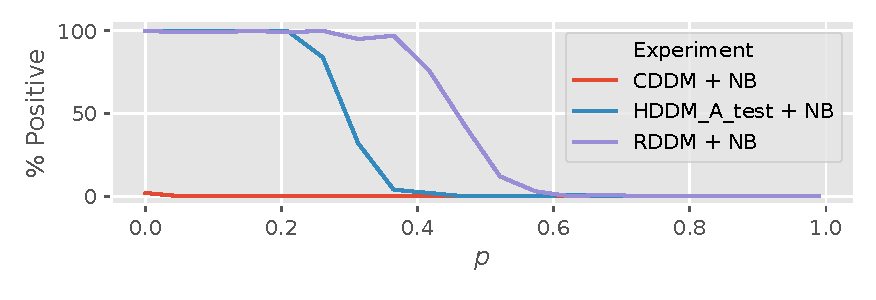
\includegraphics[width=\columnwidth]{images/vdrift_plot.pdf}
    \caption{Percentage of (false) positive drift detections for the Bernoulli data stream with virtual drift.}
    \label{fig:vdrift_plot}
\end{figure}
\begin{figure}
    \centering
    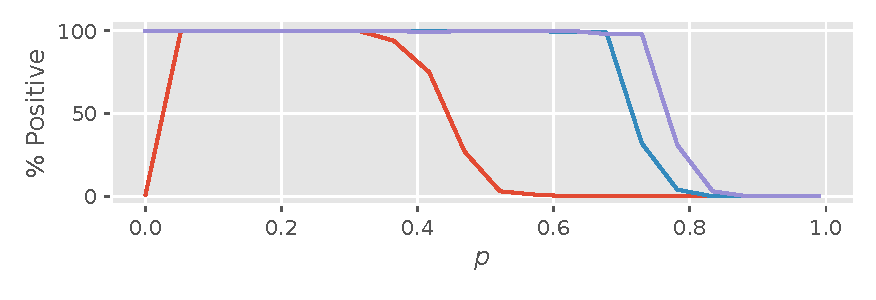
\includegraphics[width=\columnwidth]{images/rdrift_plot.pdf}
    \caption{Percentage of (true) positive drift detection for the Bernoulli data stream with real drift.}
    \label{fig:rdrift_plot}
\end{figure}


\subsection{Bernoulli-Hard}

To clearly illustrate the comparative advantage of CDDM in data streams with feature drift, we present a data stream called {\bf Bernoulli-hard}. In this data stream, we have one instance which is hard to predict, and one instance which is easy to predict. Specifically, an instance value of zero has zero noise, and an instance value of one has a noise value of 0.2. The instance rate is uniformly sampled.
\begin{align}
  \alpha &= 0 \\
  \beta &= 0.2 \\
  \gamma &\sim U[0,1]
\end{align}
When virtual drift occurs, the instance rate is reversed. When real drift occurs the one rate is reversed.
\begin{align}
  \alpha' &= 0 \\
  \beta &= 0.8 \\
  \gamma' &= 1 - \gamma
\end{align}
If the initial instance rate is less than 0.5, then after virtual drift we will see an increase in the error rate of the model due to an increase in the rate of ``hard problems". This can lead to false positives for drift detectors which use the error-rate operationalisation (henceforth ``error-rate detectors"). Conversely, when the instance rate is greater than 0.5, when real drift occurs we will see a decrease in the rate of ``hard problems", which will decrease the error rate. This may hide the increase in the error rate due to the real drift itself, and can lead to false negatives. These two scenarios are illustrated in Figure \ref{fig:bernoulli_hard}.

More specifically, the change in error rate due to feature drift will be positive when
\begin{align}
  0 &< \Delta E \\
  &< (1-\gamma)\beta - \gamma \beta \\
  &< \beta-2\gamma\beta \\
  \gamma &< 0.5.
\end{align}
Thus, any instance rate greater than 0.5 may trigger false positives in error-rate detectors. The change in error rate due to real drift is positive when
\begin{align}
  0 &< \Delta E \\
  &< (1-\gamma)(1-\beta) - \gamma\beta \\
  &< 1 - \gamma - \beta \\
  \gamma &< 0.8.
\end{align}
Thus false negatives may occur when the instance rate is above 0.8.

The results of the trials on this data stream are given in Table \ref{tab:bernoulli_hard}. We also plot the true positive, false positive and false negative rates against the instance rate to illustrate the results derived in the previous paragraph. 

\begin{figure}
    \centering
    % 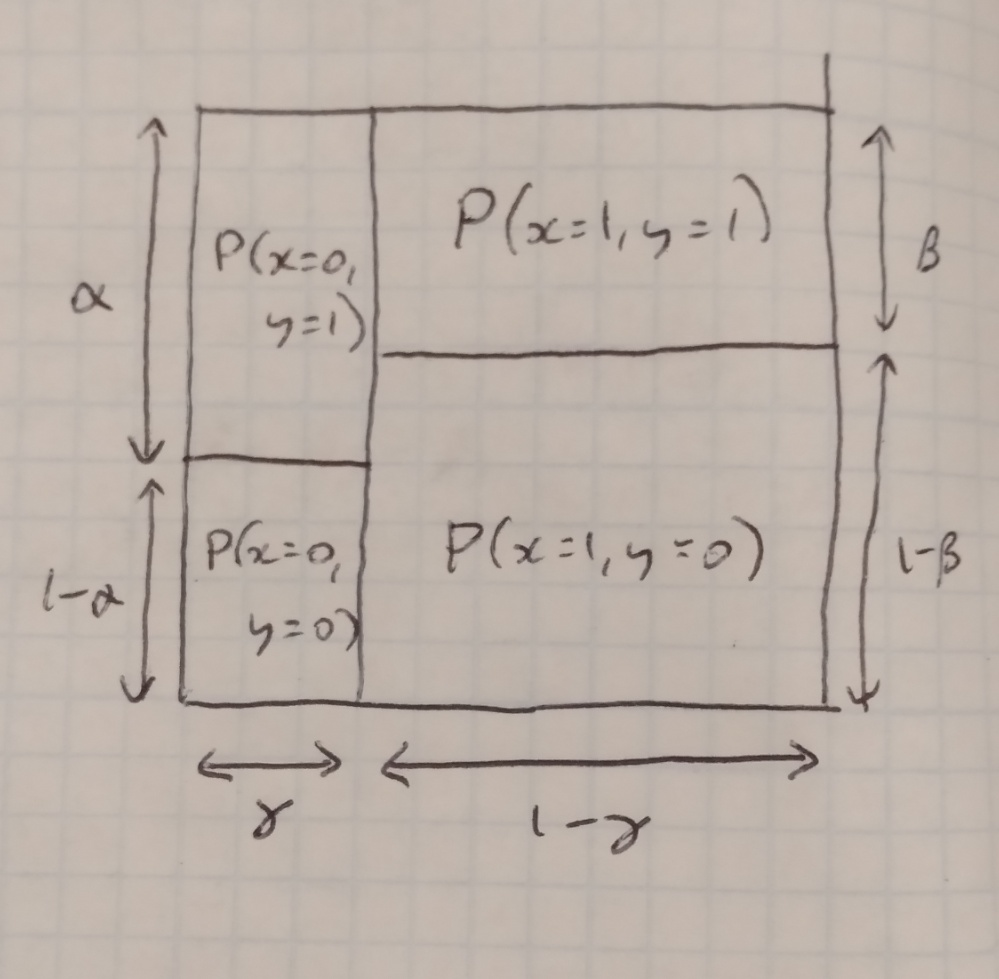
\includegraphics[width=0.5\textwidth]{images/bernoulli.jpg}
    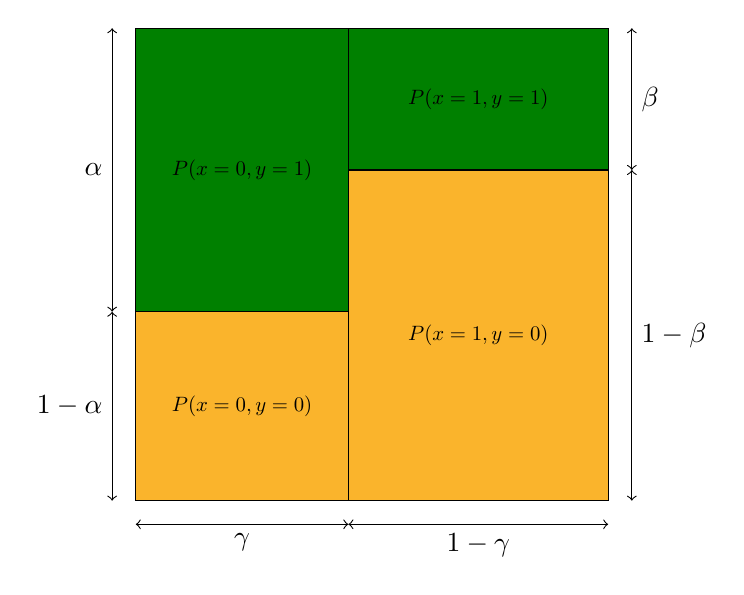
\begin{tikzpicture}[scale=6]
        %--- Arguments ----
        \def \g {0.45} % gamma
        \def \a {0.6} % alpha
        \def \b {0.3} % beta
        \def \zeroColor {Dandelion} % colour of y=0 boxes
        \def \oneColor {Green} % colour of y=1 boxes
        \def \textsep {0.05}
        %--- Rectangles ---
        \draw [fill=\zeroColor] (0,0) rectangle (\g,1-\a);
        \draw [fill=\oneColor] (0,1-\a) rectangle (\g,1);
        \draw [fill=\zeroColor] (\g,0) rectangle (1,1-\b);
        \draw [fill=\oneColor] (\g,1-\b) rectangle (1,1);
        %--- Lines ---
        % alpha
        \draw [<->] (-\textsep, 0) -- (-\textsep, 1-\a);
        \draw [<->] (-\textsep, 1-\a) -- (-\textsep, 1);
        % gamma
        \draw [<->] (0, -\textsep) -- (\g, -\textsep);
        \draw [<->] (\g, -\textsep) -- (1,-\textsep);
        % beta
        \draw [<->] (1+\textsep, 0) -- (1+\textsep, 1-\b);
        \draw [<->] (1+\textsep, 1-\b) -- (1+\textsep, 1);
        %--- Outer labels ---
        % alpha
        \node [left] at (-\textsep, 0.5-\a/2) {$1-\alpha$};
        \node [left] at (-\textsep, 1-\a/2) {$\alpha$};
        % gamma
        \node [below] at (\g/2,-\textsep) {$\gamma$};
        \node [below] at (0.5+\g/2,-\textsep) {$1-\gamma$};
        % beta
        \node [right] at (1+\textsep, 0.5-\b/2) {$1-\beta$};
        \node [right] at (1+\textsep, 1-\b/2) {$\beta$};
        %--- Inner labels ----
        \node [scale=0.75] at (\g/2,0.5-\a/2) {$P(x=0,y=0)$};
        \node [scale=0.75] at (\g/2,1-\a/2) {$P(x=0,y=1)$};
        \node [scale=0.75] at (0.5+\g/2,0.5-\b/2) {$P(x=1,y=0)$};
        \node [scale=0.75] at (0.5+\g/2,1-\b/2) {$P(x=1,y=1)$};
    \end{tikzpicture}
    \caption{Distribution of the Bernoulli data stream.}
    \label{fig:bernoulli}
\end{figure}

\begin{figure}
    \centering
    % 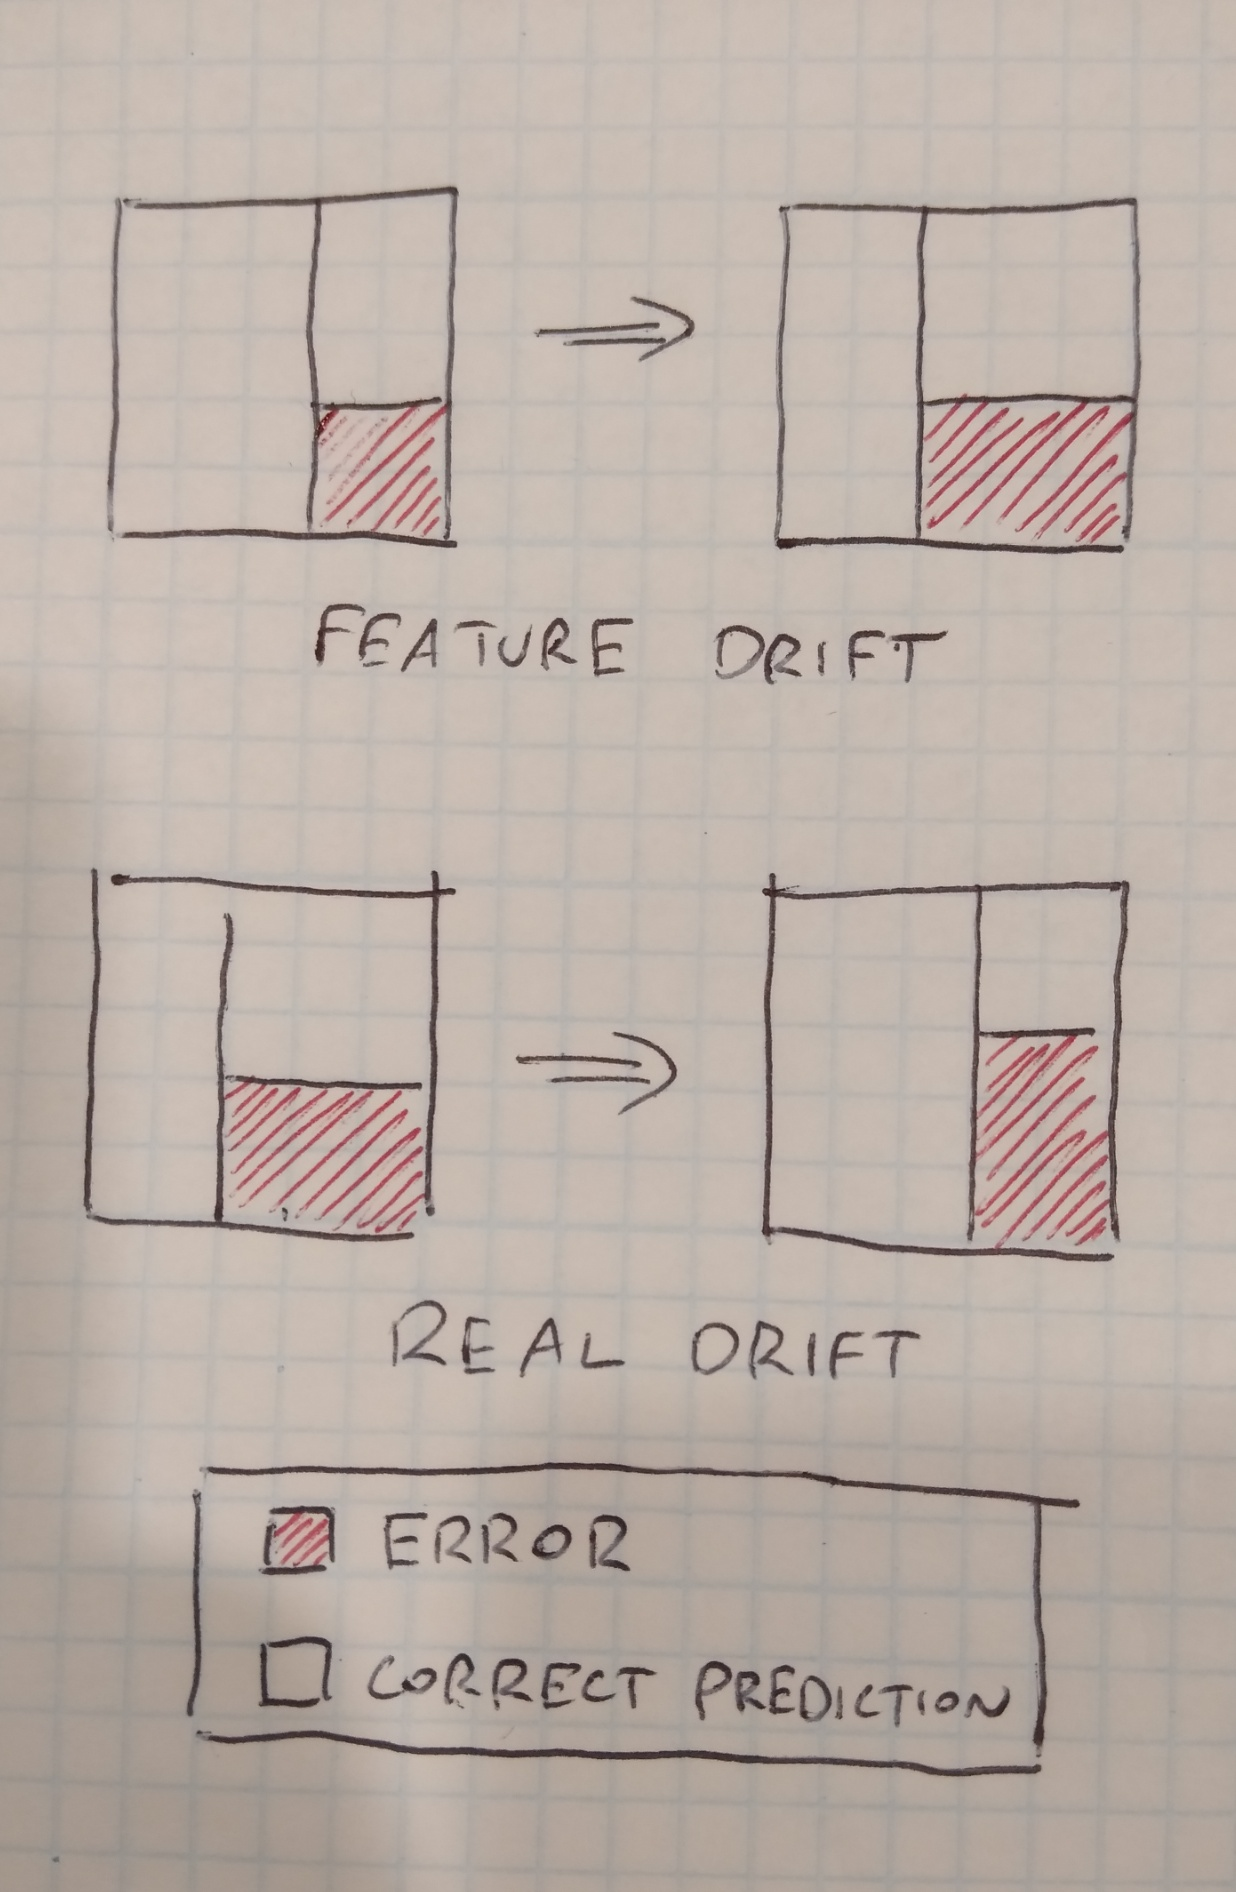
\includegraphics[width=0.5\textwidth]{images/bernoulli_hard.jpg}
    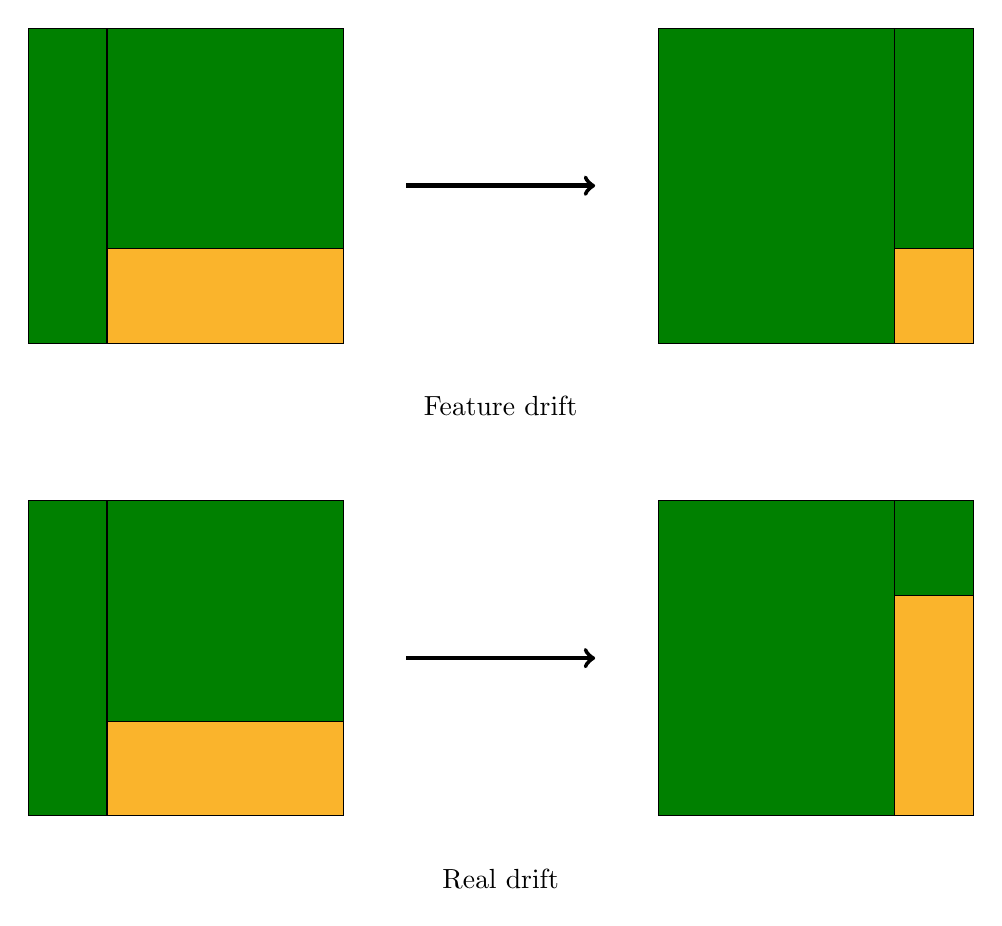
\begin{tikzpicture}[scale=4]
        % --- DEFINITIONS ---
        \def \xSep {2}
        \def \ySep {1.5}
        \def \arrowSep {0.2}
        \def \textSep {0.2}
        \def \gZero {0.25}
        \def \gOne {0.75}
        \def \bZero {0.7}
        \def \bOne {0.3}
        \def \zeroColor {Dandelion} % colour of y=0 boxes
        \def \oneColor {Green} % colour of y=1 boxes
        % \def \zeroColor {Dandelion} % colour of y=0 boxes
        % \def \oneColor {Green} % colour of y=1 boxes
        \newcommand{\bernSqr}[4]{
            % draw a Bernoulli square
            % args:
            %  x value of bottom left
            %  y value of bottom left
            %  gamma
            %  beta
            \draw [fill=\oneColor] (#1,#2) rectangle (#1+#3,#2+1);
            \draw [fill=\zeroColor] (#1+#3,#2) rectangle (#1+1,#2+1-#4);
            \draw [fill=\oneColor] (#1+#3,#2+1-#4) rectangle (#1+1,#2+1);
        }
        % --- SQUARES ---
        \bernSqr{0}{0}{\gZero}{\bZero}
        \bernSqr{\xSep}{0}{\gOne}{\bOne}
        \bernSqr{0}{\ySep}{\gZero}{\bZero}
        \bernSqr{\xSep}{\ySep}{\gOne}{\bZero}
        % --- ARROWS ---
        \draw [ultra thick, ->] (1+\arrowSep,0.5) -- (\xSep-\arrowSep,0.5);
        \draw [ultra thick, ->] (1+\arrowSep,\ySep+0.5) -- (\xSep-\arrowSep,\ySep+0.5);
        % --- TEXT ---
        \node at (0.5+\xSep/2,-\textSep) {Real drift};
        \node at (0.5+\xSep/2,\ySep-\textSep) {Feature drift};
    \end{tikzpicture}
    \caption{Distributional changes in the Bernoulli-hard data stream.}
    \label{fig:bernoulli_hard}
\end{figure}

\subsection{Bernoulli-Typical}

One may object that the previous data stream was tailor-made to showcase CDDM. We demonstrate that this is not the case with another data stream called {\bf Bernoulli-typical} which gives a much more generic picture of false positive and false negative responses from error-rate detectors. In this dataset we do not hand-pick any of the rates. Instead we sample each of them uniformly.
\begin{align}
  \alpha &\sim U[0, 0.5] \\
  \beta &\sim U[0, 0.5] \\
  \gamma &\sim U[0, 1]
\end{align}
The only constraint we place is that after real drift the zero and one rates should increase. This is because most drift detectors deliberately do not detect decreases in the error rate in case it is a result of learning. Allowing decreases in the zero and one rates would thus give CDDM an unfair advantage.
\begin{align}
  \alpha' &\sim U[\alpha, 1] \\
  \beta' &\sim U[\beta, 1] \\
  \gamma' &\sim U[0, 1]
\end{align}

The results of the trials on this data stream are given in Table \ref{tab:bernoulli_hard}.

%-------------------------------------------------------------------
% BENCHMARK DATASETS
%-------------------------------------------------------------------

\section{Benchmark Datasets} \label{Experiments:benchmark}

In this section we evaluate the concept drift detection methods we have introduced on a battery of benchmark datasets. The Tornado framework provides implementations of the following synthetic data streams:
\begin{itemize}
    \item {\bf CIRCLES} Each instance consists of two attributes $x_1,x_2\sim U[0,1]$. Each concept consists of three values, $r,x_{circ},y_{circ}\in[0,1]$, representing the radius of a circle, and $x$ and $y$ coordinates of the center of a circle. And instance is given a positive label if it falls within the circle, otherwise it is given a negative label. Sampling is done such that an equal number of positive and negative instances occur. The concept parameters cycle through the values of $[0.15, 0.2, 0.5]$, $[0.2, 0.4, 0.5]$, $[0.25, 0.6, 0.5]$ and $[0.3, 0.8, 0.5]$.
    \item {\bf LED} Each concept in the LED task is a digit displayed on a 7-bit LED interface. There are 10 labels (the digits $0,1,2,\dots,9$) and 7 binary features (each of the display bits).  For example, the label corresponding to the instance [1, 1, 1, 1, 1, 1, 0] is $0$. In addition to the concept bits, there are also $n$ irrelevant and random-valued binary attributes. The position of the irrelevant attributes changes with each concept, so the model must learn anew which attributes are decision-relevant. 
    \item {\bf MIXED} Each instance is a mix of two binary attributes $w,v\in\{0,1\}$, and two real-valued attributes $x_1,x_2\sim U[0,1]$. Labels are assigned according to $y=\mathrm{1}[v \wedge w \wedge  y < 0.5 + 0.3 \sin(3\pi x)]$. After each context change the classification is reversed.
    \item {\bf SEA} Each instance consists of three attributes $x_1,x_2,x_3\sim U[0,10]$. Each concept consists of a threshold $\theta$, such that $y=\mathrm{1}[x_1+x_2+x_3 > \theta]$. That is, if the binary label denotes whether the sum of the attributes exceeds the threshold. Thresholds cycle between the values $[8, 9, 7, 9.5]$.
    \item {\bf SINE1} Each instance consists of two attributes $x_1,x_2\sim U[0,1]$. Binary labels are given by $y = \mathrm{1}[x_1>sin(x_2)]$. When concept drift occurs, the labels are reversed.
    \item {\bf SINE2} As with SINE1, the attributes are $x_1,x_2\sim U[0,1]$. Binary labels are given by $y = \mathrm{1}[x_1>0.5+0.3\sin(3\pi x_2)]$. When concept drift occurs, the labels are reversed.
    \item {\bf STAGGER} Instances consist of categorical attributes $size\in [small, medium, large]$, $color\in [red, green]$, $shape\in [circular, non-circular]$. Each concepts is a first order logic expression. Specifically, the following concepts are cycled: $y=\mathrm{1}[size=small \wedge color=red]$, $y=\mathrm{1}[color=green \vee shape=circular]$, and $y=\mathrm{1}[size=medium \vee size=large]$.
\end{itemize}
These data streams provide constitute the most popular benchmarks used in the concept drift detection literature. Each of these data streams has the following parameters:
\begin{itemize}
    \item {\bf Concept Length} The number of instances between concept drifts. If this number is small then the data stream is {\it volatile}, if this number is small then the data stream is {\it stable}.
    \item {\bf Transition Length} The number of instances over which a concept drift occurs. If the transition length is $n$, and there have been $i$ instances since the concept drift, then the probability that the new concept is used is $P(new-concept)=i/n$, otherwise the previous concept is used. If the transition length is low then the drift is {\it abrupt}. Otherwise the stream is {\it gradual}.
    \item {\bf Noise Rate} The rate at which any given label will be replaced with a different label. For binary labels, the label is simply inverted. Otherwise, a different label is chosen at random. If this quantity is high, then the data stream is {\it noisy}.
\end{itemize}
We are interested in how drift detector performance varies with noise and transition length. We therefore run experiments using each of the variations of the above datasets
\begin{itemize}
    \item {\bf High Noise} Noise rate is set to 0.4, transition length is set to 50 and concept length is set to 1000.
    \item {\bf Low Noise} Noise rate is set to 0.02, transition length is set to 50 and concept length is set to 1000.
    \item {\bf Gradual Drift} Transition length is set to 250, noise rate is set to 0.1, and concept length is set to 1000.
    \item {\bf Abrupt Drift} Transition length is set to 0, noise rate is set to 0.1, and concept length is set to 1000.
    \item {\bf Long concepts} Transition length is set to 50, noise rate is set to 0.1, and concept length is set to 25000.
    \item {\bf Short concepts} Transition length is set to 50, noise rate is set to 0.1, and concept length is set to 250.
\end{itemize}
We run each datastream with two base learners. Na\"{i}ve Bayes and Hoeffding trees \cite{hoeffding_trees} are two of the most popular, so we use these.  

We run two iterations of each of the 7 data streams, for each of the four variations, with both of the base learners. The results are given in Table \ref{tab:benchmarks} and visualised in Figure \ref{fig:benchmarks}. 

\begin{sidewaystable}
    \centering
    \caption{Results of benchmark datasets.}
    \begin{tabular}{lrrrrrr}
\toprule
{} &         Precision &            Recall &                F1 &          Mean Delay &              Memory (bytes) &            Runtime (ms) \\
Detector     &                   &                   &                   &                     &                     &                    \\
\midrule
ADWIN        &       0.49 (0.20) &       0.50 (0.26) &       0.47 (0.23) &      173.56 (76.56) &       59.78 (73.15) &      60.27 (62.47) \\
BWAF         &       0.59 (0.17) &       0.63 (0.23) &       0.60 (0.19) &      105.20 (84.93) &       52.56 (76.53) &     86.75 (109.54) \\
CDDM         &       0.40 (0.27) &       0.61 (0.27) &       0.38 (0.27) &      132.92 (93.41) &      78.19 (141.79) &     81.65 (179.35) \\
CUSUM        &       0.64 (0.18) &       0.51 (0.28) &       0.55 (0.24) &      194.15 (61.85) &      68.20 (144.00) &     84.61 (133.74) \\
DDM          &       0.67 (0.16) &       0.57 (0.27) &       0.60 (0.23) &      149.43 (81.68) &      61.87 (113.65) &     78.30 (121.63) \\
EDDM         &       0.47 (0.20) &       0.60 (0.25) &       0.50 (0.21) &      141.65 (76.42) &      60.95 (115.77) &     64.53 (111.05) \\
EWMA         &       0.48 (0.18) &       0.60 (0.23) &       0.51 (0.18) &      112.58 (84.33) &       47.32 (45.72) &     70.33 (168.48) \\
FHDDM        &       0.57 (0.18) &       0.66 (0.21) &       0.60 (0.18) &      114.97 (67.17) &       54.17 (89.55) &      49.37 (92.55) \\
FHDDMS       &       0.49 (0.20) &       0.67 (0.19) &       0.54 (0.18) &      110.00 (64.19) &       48.35 (49.73) &      44.40 (80.51) \\
FHDDMS$_{add}$   &       0.17 (0.12) &  {\fontseries{b}\selectfont 0.79 (0.06)} &       0.26 (0.14) &  {\fontseries{b}\selectfont 76.39 (37.31)} &  {\fontseries{b}\selectfont 41.05 (41.47)} &  {\fontseries{b}\selectfont 7.59 (13.95)} \\
HDDM$_A$  &  {\fontseries{b}\selectfont 0.68 (0.16)} &       0.60 (0.26) &       0.62 (0.23) &      129.86 (88.14) &      59.99 (108.88) &     72.75 (103.00) \\
HDDM$_W$  &       0.65 (0.19) &       0.63 (0.23) &  {\fontseries{b}\selectfont 0.63 (0.21)} &      116.21 (82.71) &      60.97 (109.85) &     65.47 (102.01) \\
MDDM$_A$   &       0.55 (0.18) &       0.65 (0.20) &       0.58 (0.17) &      115.83 (65.88) &       52.02 (80.13) &      62.35 (94.20) \\
MDDM$_E$   &       0.53 (0.19) &       0.64 (0.21) &       0.56 (0.18) &      118.31 (69.11) &       47.42 (44.77) &      54.25 (88.08) \\
MDDM$_G$   &       0.53 (0.19) &       0.64 (0.20) &       0.57 (0.18) &      117.62 (66.90) &       47.27 (44.61) &      54.95 (88.30) \\
Null &       0.50 (0.00) &       0.19 (0.03) &       0.28 (0.03) &       249.98 (0.15) &      84.39 (159.77) &    200.90 (383.73) \\
PH  &       0.50 (0.19) &       0.34 (0.23) &       0.39 (0.21) &      231.80 (31.77) &      75.09 (150.22) &    122.89 (231.97) \\
RDDM         &       0.66 (0.18) &       0.62 (0.25) &       0.63 (0.22) &      127.33 (84.36) &      113.81 (83.46) &     66.14 (104.59) \\
SeqDrift2    &       0.44 (0.20) &       0.43 (0.24) &       0.41 (0.20) &      204.78 (51.88) &     117.58 (155.47) &      56.49 (64.58) \\
\bottomrule
\end{tabular}

    \label{tab:benchmarks}
\end{sidewaystable}

\begin{figure}
    \centering
    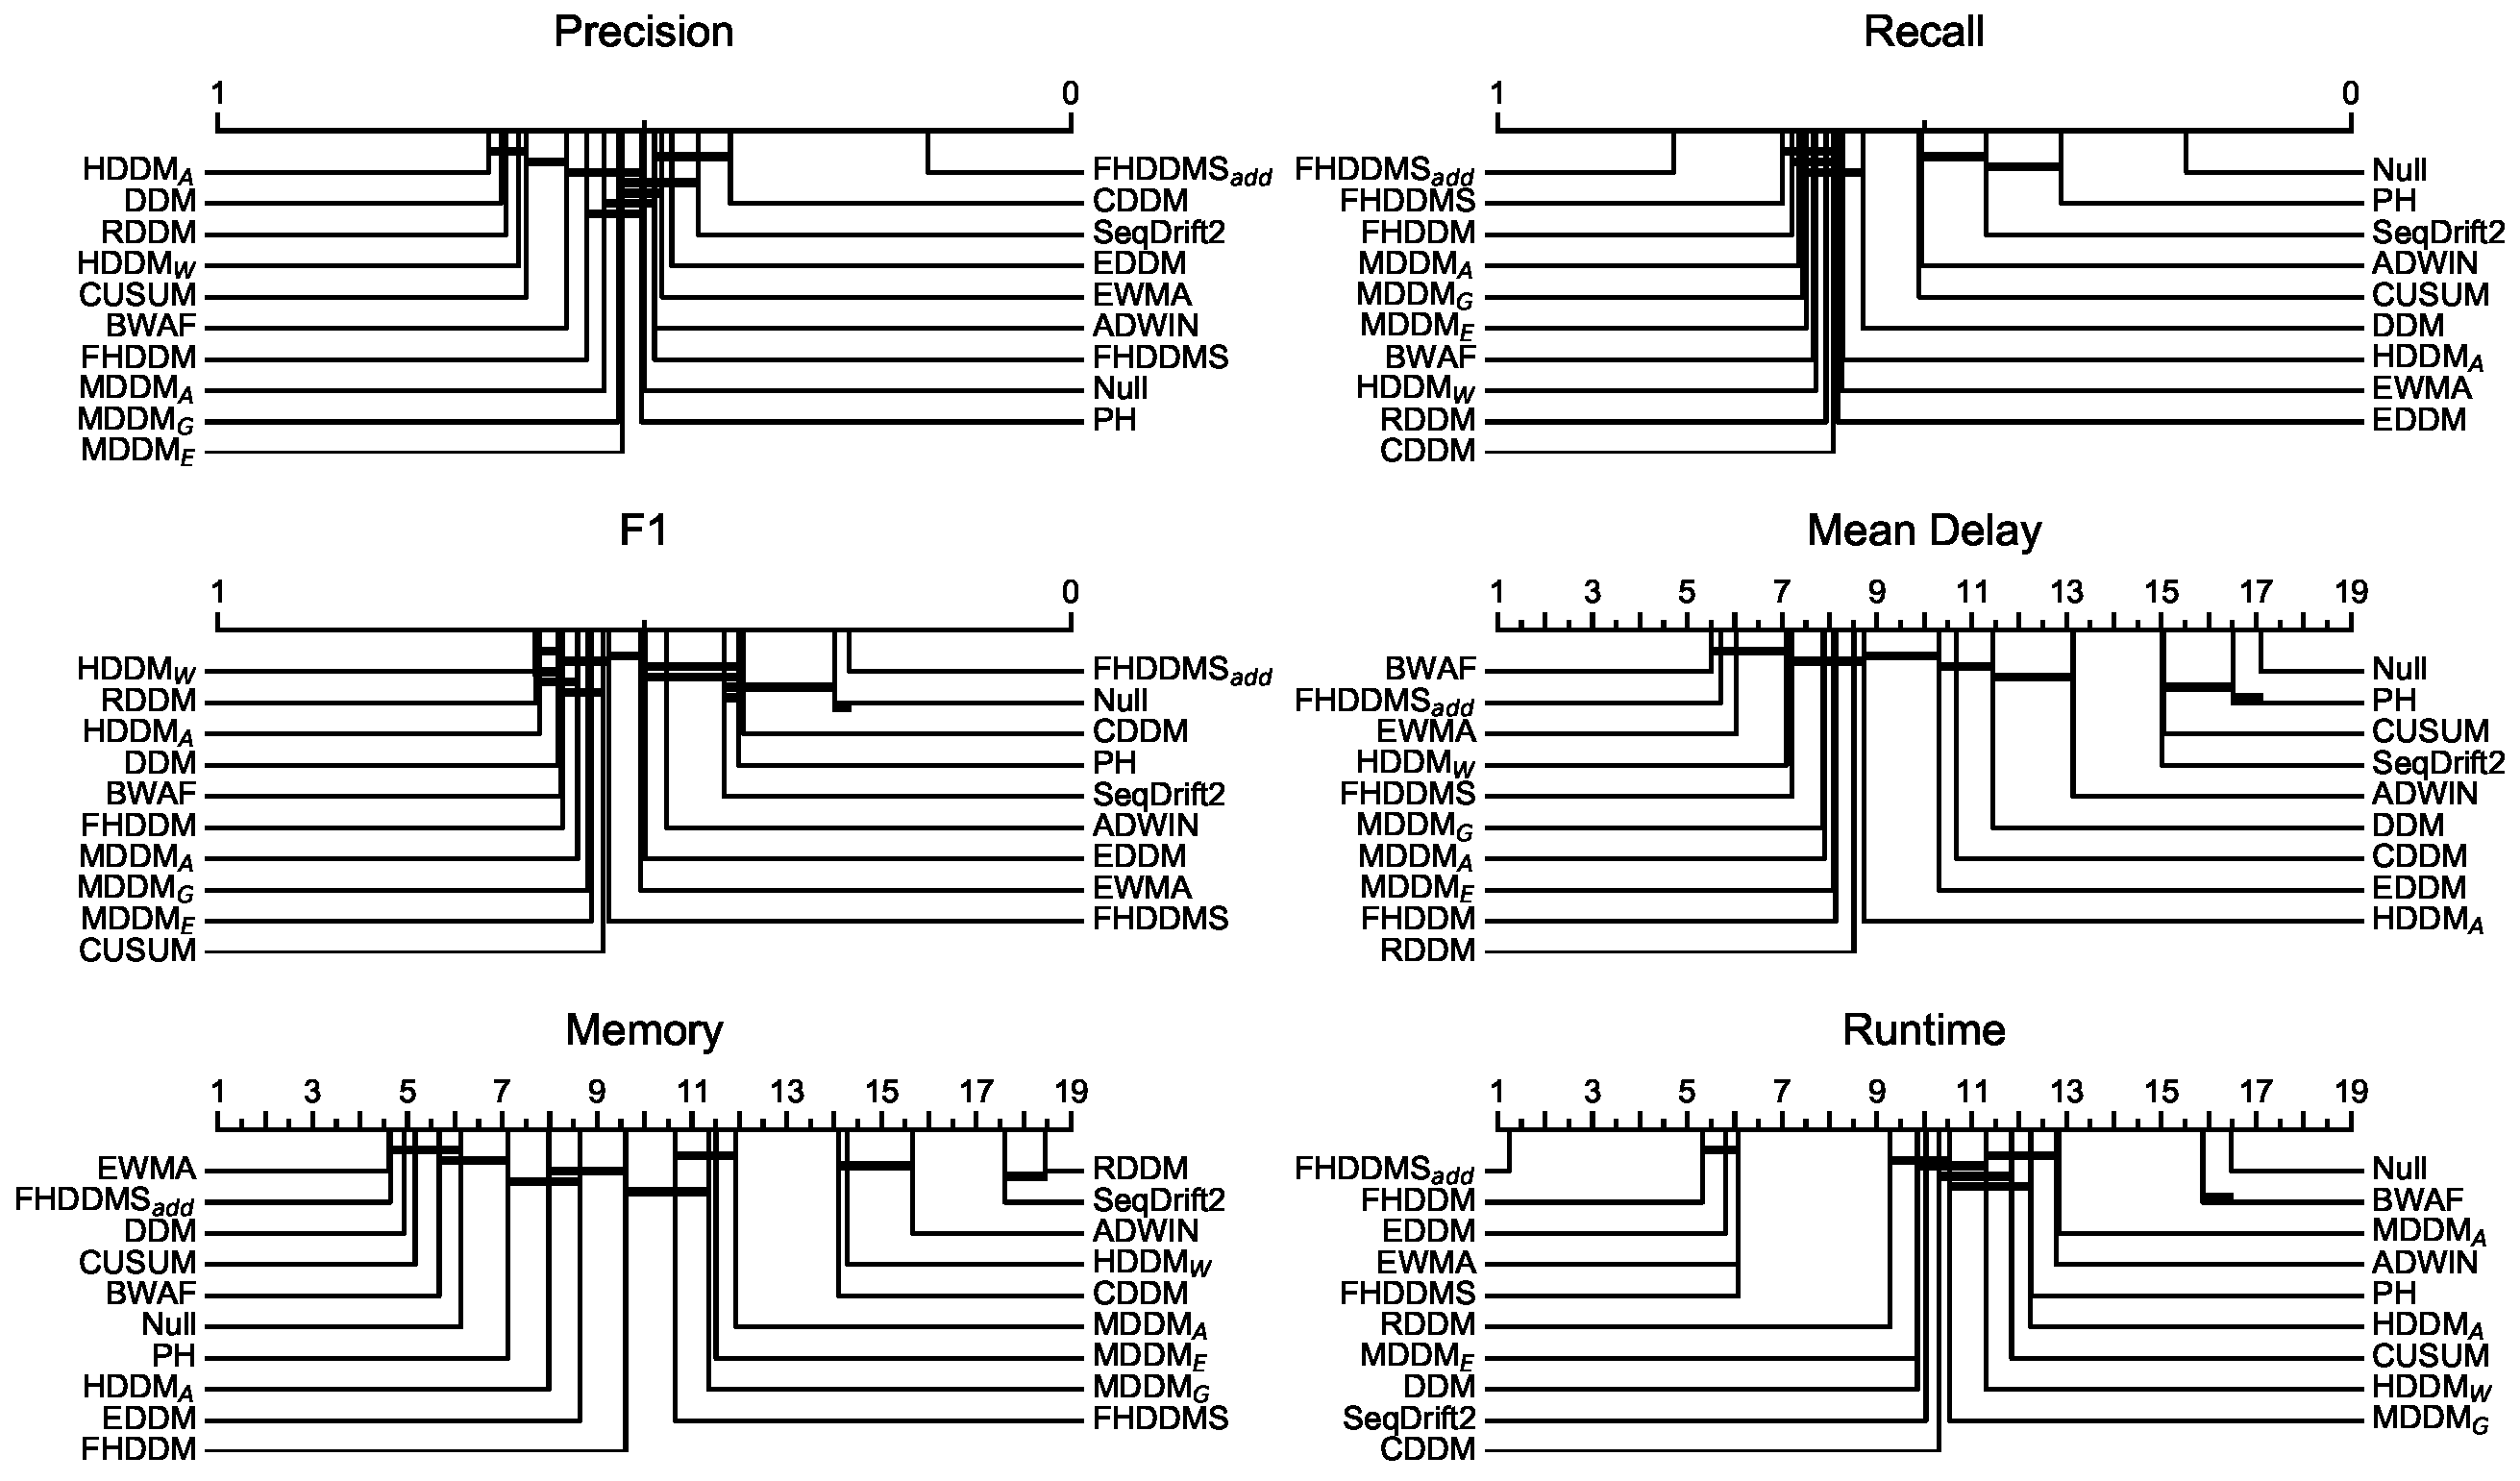
\includegraphics[width=\textwidth]{images/cd_diagrams/benchmark.pdf}
    \caption{CD diagram of benchmark datasets.}
    \label{fig:benchmarks}
\end{figure}

We see that BWAF performs well on benchmark datasets. It achieves the fifth highest precision (significantly less than the best detector at $p<0.05$), the seventh best recall (not significantly less than the best detector at $p<0.05$), the fourth best F$_1$ score (not significantly less than the best detector at $p<0.05$), the best mean delay (although not significantly greater than the second best at $p<0.05$), the fifth best memory consumption (not significantly worse than the best detector at $p<0.05$), but the second worst runtime.

By contrast, the performance of CDDM is poor. Because the instances in these data streams are high dimensional, the learners are uncalibrated, triggering a high rate of false positives. On recall and memory, CDDM is ranked in the middle the detectors. On all other metrics it is in the lower half of detectors. This affirms the statement in Section \ref{CDDM:conclusion} that CDDM must be extended with online calibration for practical usage.

%-------------------------------------------------------------------
% SYNTHETIC MEDICAL
%-------------------------------------------------------------------

\section{Triage Simulation} \label{Experiments:triage}

In this section we evaluate our novel concept drift detectors in the motivating example domain of GP referrals triage. Due to a lack of real triage data annotated by concept drift, we instead use a synthetic data stream with concept drift deliberately introduced.

We base our synthetic data stream on the MIMIC-III dataset - a publicly available repository of free-text electronic health records \cite{mimic}. There are several types of documents within the dataset, so we limit our usage to `radiology' documents, which have the advantage of having structured headers. We preprocess the 522,279 radiology documents by converting the text into bag-of-words format. To keep the instance dimensionality reasonable, we eliminate tokens which occur in fewer than 40\% or more than 60\% of documents, resulting in 59,652 dimensional features. We shuffle the order of the documents to make sure the only concept drifts which occurs in the data stream have been deliberately engineered.

To simulate a triage rule, we randomly label 30 referral documents with priority labels 1 to 4. We then train a decision tree on these instance-label pairs. We repeat this several times to obtain a set of ``triage concepts". Concept drift is simulated by labelling the instances prior to the drift point using one triage concept, and then labelling the instances after the drift with another, randomly selected concept. In each instantiation of the data stream a single concept drift occurs halfway through the stream.

We run two iterations of the medical triage data stream under each of the variations described in Section \ref{Experiments:benchmark}, namely high noise, low noise, gradual drift, abrupt drift, long concepts, short concepts. The results are given in Table \ref{tab:triage} and visualised in Figure \ref{fig:triage}. 

\begin{sidewaystable}
    \centering
    \caption{Results of synthetic triage data streams.}
    \begin{tabular}{lrrrrrr}
\toprule
{} &         Precision &            Recall &                F1 &          Mean Delay &                 Memory (bytes) &               Runtime (ms) \\
Detector     &                   &                   &                   &                     &                        &                       \\
\midrule
ADWIN        &       0.45 (0.13) &       0.52 (0.17) &       0.48 (0.14) &      184.53 (72.04) &      2071.95 (2703.76) &     1188.44 (1201.33) \\
BWAF         &       0.61 (0.11) &       0.64 (0.09) &       0.61 (0.09) &       64.92 (70.37) &      2031.33 (3074.38) &      1074.40 (890.51) \\
CDDM         &       0.11 (0.19) &       0.60 (0.13) &       0.11 (0.14) &       65.22 (97.95) &      1202.42 (1182.93) &       326.97 (790.04) \\
CUSUM        &       0.50 (0.14) &       0.44 (0.16) &       0.47 (0.14) &      216.06 (50.18) &      2180.51 (3042.57) &     1273.14 (1099.90) \\
DDM          &       0.57 (0.13) &       0.55 (0.16) &       0.56 (0.15) &      176.42 (64.35) &      2212.87 (3177.23) &     1182.96 (1092.59) \\
EDDM         &       0.38 (0.18) &       0.48 (0.17) &       0.41 (0.16) &      191.56 (79.70) &      2017.23 (2741.34) &      1047.99 (985.13) \\
EWMA         &       0.47 (0.14) &       0.52 (0.17) &       0.48 (0.13) &     136.42 (110.62) &      1790.92 (2524.41) &      1038.35 (982.84) \\
FHDDM        &       0.33 (0.14) &       0.60 (0.13) &       0.41 (0.12) &      100.25 (87.19) &      1594.83 (1881.50) &       489.60 (381.47) \\
FHDDMS       &       0.21 (0.11) &       0.60 (0.13) &       0.30 (0.11) &       97.19 (90.45) &       1208.86 (976.79) &       292.01 (222.99) \\
FHDDMS$_{add}$   &       0.16 (0.10) &  {\fontseries{b}\selectfont 0.67 (0.00)} &       0.25 (0.11) &  {\fontseries{b}\selectfont 62.39 (51.61)} &  {\fontseries{b}\selectfont 1122.88 (841.49)} &  {\fontseries{b}\selectfont 156.54 (110.67)} \\
HDDM$_A$  &       0.60 (0.11) &       0.56 (0.15) &       0.58 (0.13) &      122.89 (94.24) &      2178.58 (3180.54) &     1217.33 (1110.18) \\
HDDM$_W$  &       0.44 (0.11) &       0.59 (0.14) &       0.50 (0.11) &       83.36 (99.85) &      1987.08 (2840.06) &       922.85 (872.30) \\
MDDM$_A$   &       0.30 (0.14) &       0.57 (0.15) &       0.38 (0.13) &      105.22 (94.68) &      1586.03 (1860.45) &       490.82 (378.84) \\
MDDM$_E$   &       0.30 (0.13) &       0.58 (0.14) &       0.38 (0.12) &      103.72 (93.50) &      1561.36 (1640.40) &       462.48 (340.40) \\
MDDM$_G$   &       0.31 (0.12) &       0.60 (0.13) &       0.39 (0.12) &       93.47 (89.14) &      1565.05 (1858.74) &       473.55 (349.91) \\
Null &       0.50 (0.00) &       0.33 (0.00) &       0.40 (0.00) &       250.00 (0.00) &      2156.45 (3465.22) &     2181.42 (2075.25) \\
PH  &       0.44 (0.10) &       0.35 (0.08) &       0.39 (0.07) &      244.67 (21.99) &      2112.62 (3124.96) &     1594.42 (1440.53) \\
RDDM         &  {\fontseries{b}\selectfont 0.63 (0.07)} &       0.63 (0.10) &  {\fontseries{b}\selectfont 0.63 (0.09)} &      116.64 (66.99) &      2117.44 (3076.81) &      1078.29 (993.25) \\
SeqDrift2    &       0.46 (0.11) &       0.46 (0.16) &       0.45 (0.12) &      208.89 (58.49) &      1994.71 (2702.04) &     1440.93 (1548.25) \\
\bottomrule
\end{tabular}

    \label{tab:triage}
\end{sidewaystable}

\begin{figure}
    \centering
    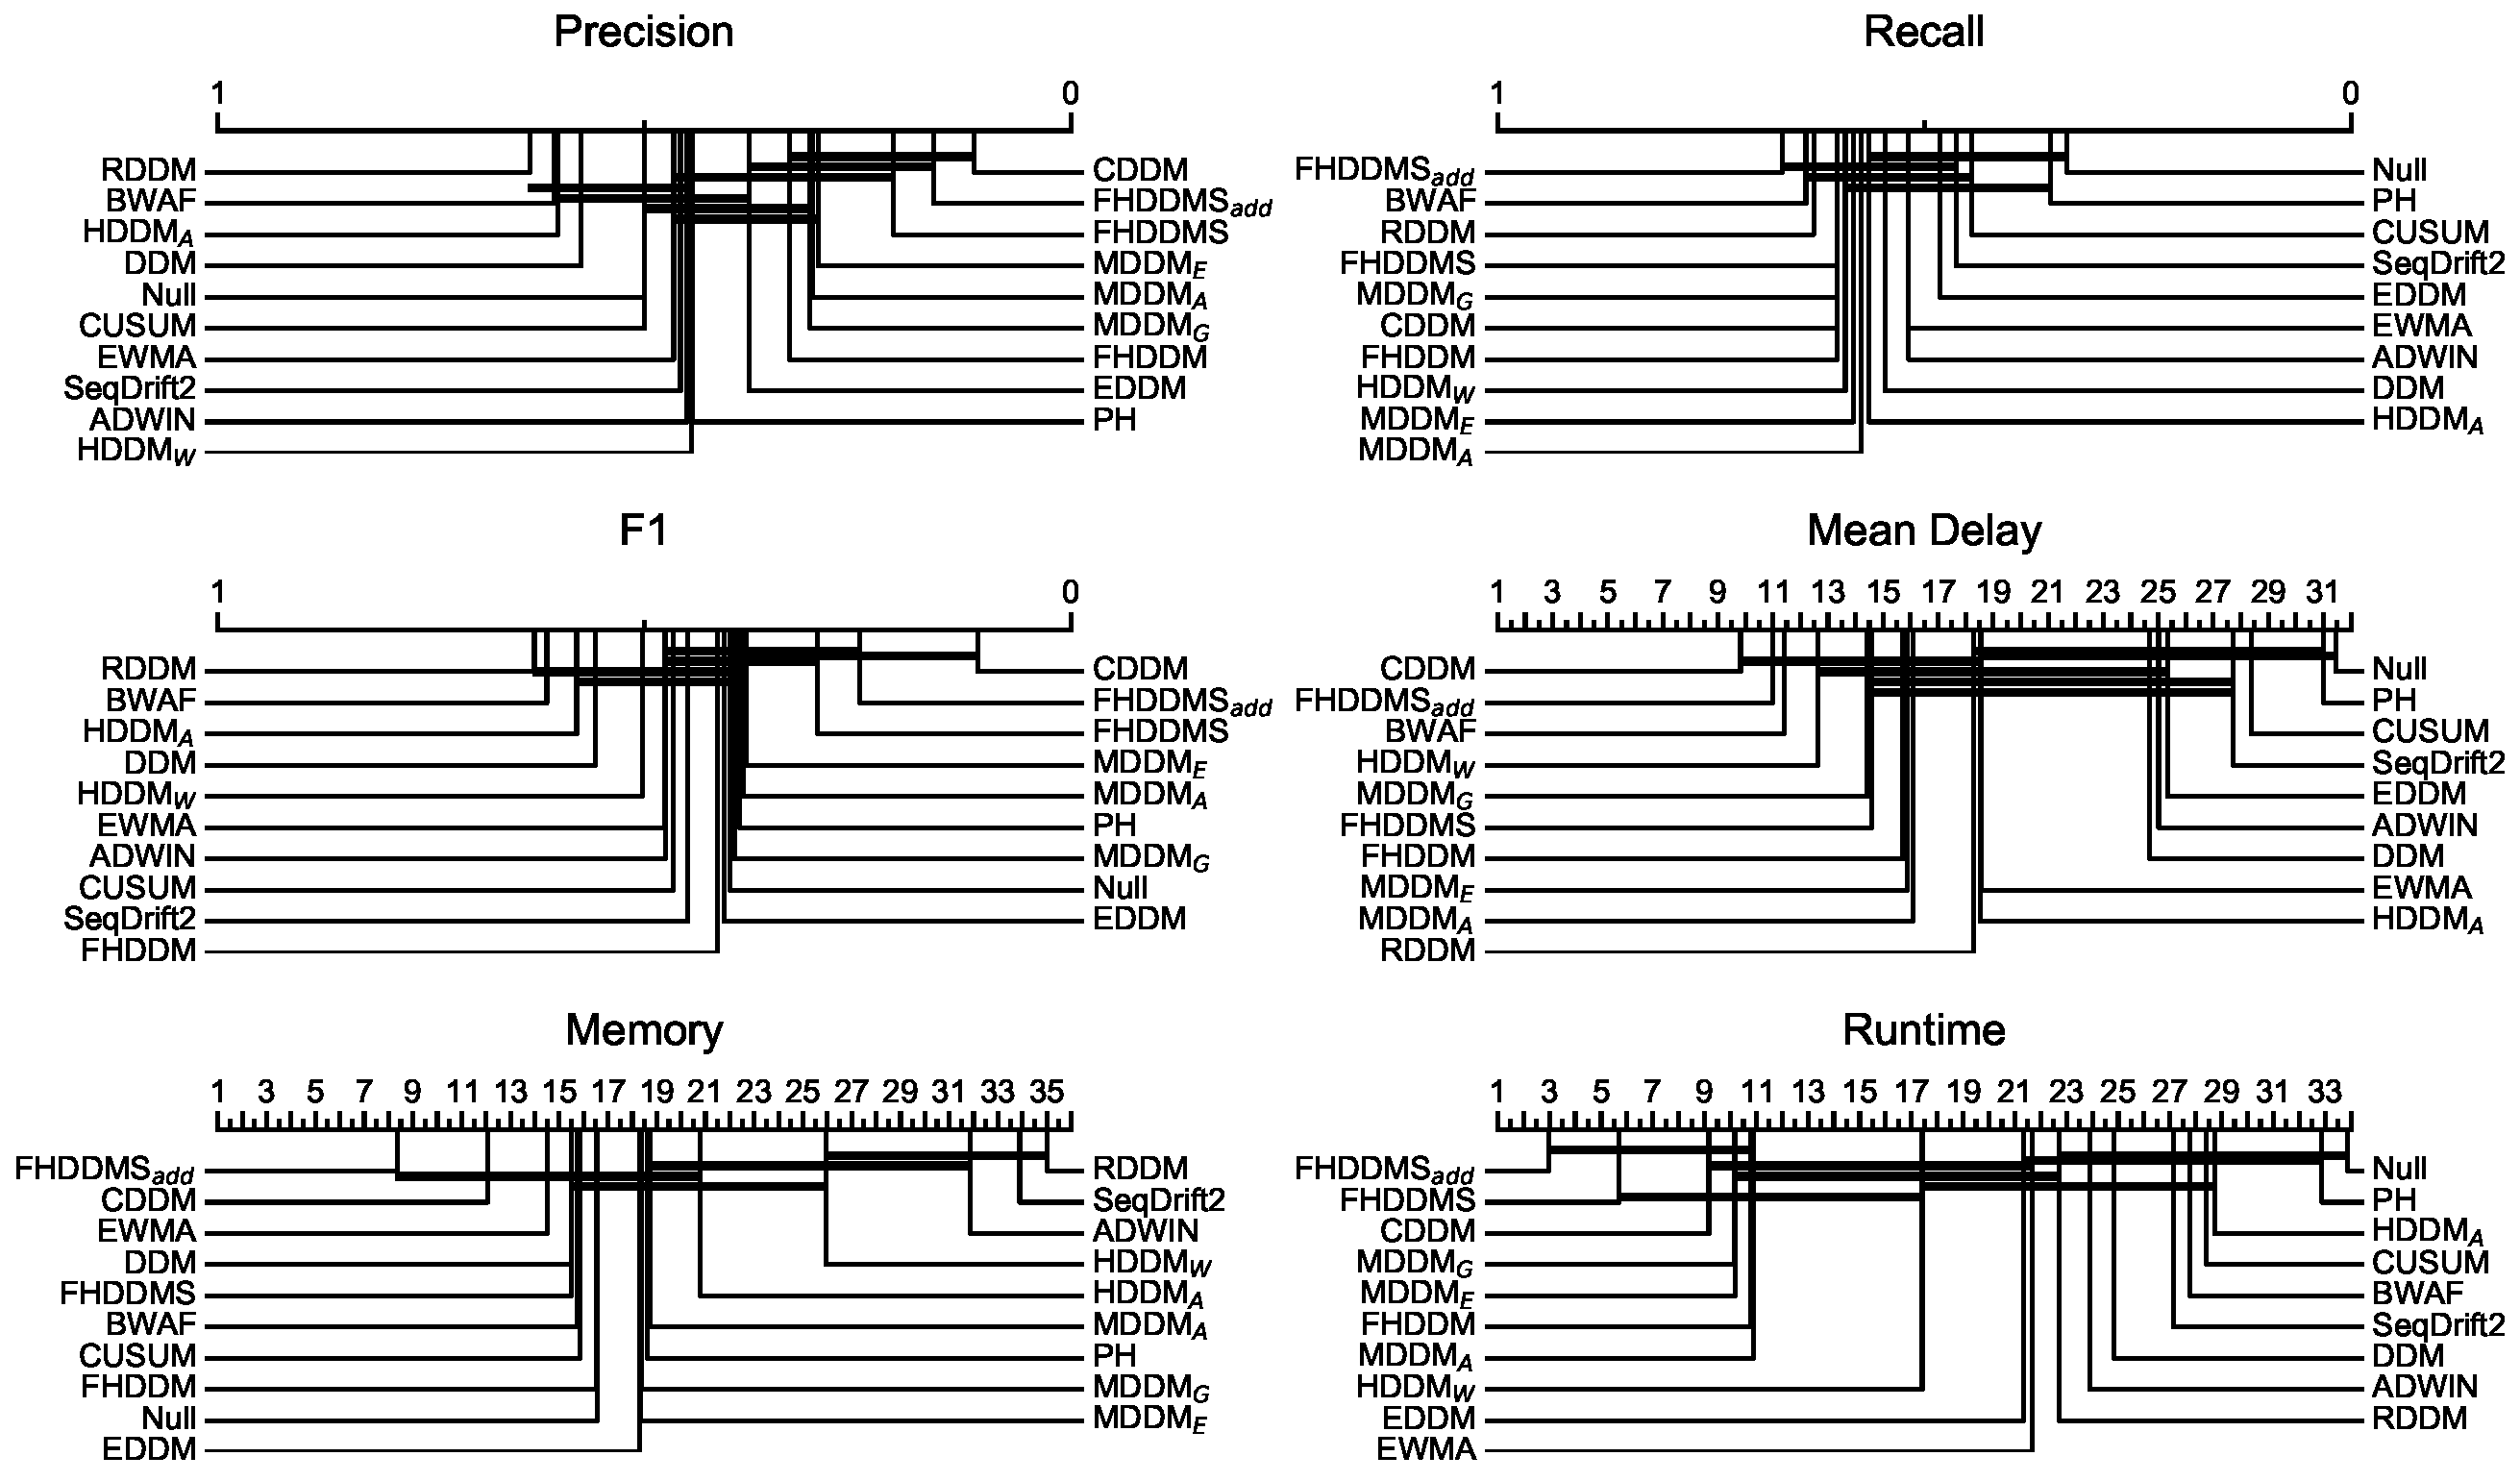
\includegraphics[width=\textwidth]{images/cd_diagrams/mimic.pdf}
    \caption{CD diagram of synthetic triage data streams.}
    \label{fig:triage}
\end{figure}

Similar to Section \ref{Experiments:benchmark}, we see competitive performance from BWAF. It achieves the second highest precision, recall, and F$_1$ score, as well as the third best mean delay (none of which is significantly worse than the best detector at $p<0.05$). The memory consumption is sixth best (not significantly less than the best detector at $p<0.05$), although the runtime is fifth worst.

As in Section \ref{Experiments:benchmark}, the performance of CDDM is poor. CDDM achieved the worst precision and F$_1$ of all the detectors, although it achieved the sixth best recall, the best mean delay, the second best memory consumption, and the third lowest runtime. As before, this poor performance can be attributed to the models being miscalibrated, a problem which is especially acute given the high dimensionality of the data. 

%-------------------------------------------------------------------
% CONCLUSION
%-------------------------------------------------------------------

\section{Conclusion} \label{Experiments:conclusion}

In this chapter we experimentally validated our novel drift, and investigated the performance of drift detectors on a synthetic medical triage dataset. We have seen that BWAF is a competitive drift detector on a battery of benchmark data streams, and a synthetic GP referrals triage data stream. It consistently achieved one of the best precision, recall, F$_1$, detection delays scores. BWAF's memory usage reasonable, consistently within the top quartile, although its runtime was generally not competitive. CDDM did not perform competitively in these experiments. We attribute this to the models being uncalibrated, thus affirming the claim made in Section \ref{CDDM:conclusion} that CDDM should be combined with online calibration for practical usage.
\chapter{Conclusion} \label{chapt:Conclusion}

In this chapter we summarise our work and promising future work. Section \ref{conclusion:achievements} highlights major achievements of this thesis. Section \ref{conclusions:limitations} identifies the main limitations of our work. Section \ref{conclusions:future_word} discusses the most promising future work.

%-------------------------------------------------------------------
% ACHIEVEMENTS
%-------------------------------------------------------------------

\section{Achievements} \label{conclusion:achievements}

The following list highlights the major achievements of our research:

\noindent{\bf Chapter \ref{chapt:MDD}}
\begin{itemize}
  \item We introduced multiple drift detector (MDD), a framework  for monitoring for several types of concept drift, specifically real drift, label drift, and feature drift.
  \item This allows users to receive early warnings that a model is no longer fit for purpose due to changes in the instance distribution, so that the model can be recalled if necessary.   
  \item MDD is flexible and can be implemented using any existing drift detection method.
  \item We also introduced a graphical interface for visualising the evolution of the data stream.
%   introduced a framework for providing early warnings that a model requires retraining or recall, the multiple drift detector (MDD). MDD monitors the instance distribution, the label distribution, {\it and} the instance-label joint distribution for signs of drift. MDD is constructed out of an ensemble of existing drift detectors, and has significant flexibility in its implementation. We also present a graphical interface for visualising the history of the status of MDD.
\end{itemize}
{\bf Chapter \ref{chapt:CDDM}}
\begin{itemize}
  \item We introduced calibrated drift detection method (CDDM), a drift detector which only detects reducible, and not irreducible, performance degradation. 
  \item CDDM is thus able to avoid false positives due to feature drift which do not change the decision boundary. In these cases, retraining the model is at best pointless and at worst detrimental due to reducing the size of the training data.
  \item We demonstrated the value of CDDM by achieving the highest F$_1$ score on a Bernoulli data stream with feature drift and variation in prediction difficulty.
\end{itemize}
{\bf Chapter \ref{chapt:BDD}}
\begin{itemize}
  \item We introduced Bayesian drift detection method (BDDM), a method for exactly calculating posterior probabilities of drift timing and performance degradation. 
  \item This allows user to make more rational decisions about model retraining, based on expected utility. 
  \item BDDM is able to accommodate uneven time series, by factoring the spaces between instances into prior values.
  \item We also introduce beta with adaptive forgetfulness (BWAF), an efficient heuristic approximation of BDDM. BWAF requires only four registers of memory, and has $O(1)$ computational complexity. It also does not require parameter selection. 
  \item BWAF was shown to be competitive on standard benchmarks, achieving the second highest F$_1$ score. It was also competitive on the synthetic triage data stream, again achieving the second highest F$_1$ score.
%   \item We introduced a drift detection method which calculates exact posterior probabilities of concept drift having occurred at each time step, Bayesian drift detection method (BDDM). It also calculates posterior distributions over the values of performance metrics both before and after the occurrence concept drift.
%   \item We also introduced beta with adaptive forgetfulness (BWAF), an efficient heuristic-based drift detection method inspired by BDDM. BWAF computes posterior probabilities of drift having occurred, although unlike BDDM, the posteriors for past time steps are not updated in light of new evidence. It is, however, very space and time efficient. It also does not require parameter tuning.
\end{itemize}

%-------------------------------------------------------------------
% LIMITATIONS
%-------------------------------------------------------------------

\section{Limitations} \label{conclusions:limitations}

We identify the following major limitations of this work.

\subsection{Multiple Drift Detector}

The purpose of this system was to provide early warnings of feature drift when label values are delayed compared to feature values. However, there are limitations to the types of feature drifts which can be detected. 

By representing free-text features as bags of words, all information about the arrangement of tokens is lost, and so only changes at the token-frequency level are detectable. MDD also assumes independence between features. Thus changes in the correlation between features are undetectable by MDD.

\subsection{Calibrated Drift Detection Method}

In Chapter \ref{chapt:CDDM}, we identified two limitations of CDDM. The first was that it cannot detect ``small" deviations from miscalibration. The minimum detectable deviation depends on the window size and the detection threshold, as specified in Equation \ref{eq:window_size}. 

The second limitation is that CDDM requires its model to be calibrated. Most machine learning methods require post-processing of probabilistic predictions to become calibrated \cite{calibrating}, and these can require large amounts of training data to achieve \cite{beyond_sigmoids} and are not necessarily robust against dataset drift \cite{dataset_drift}. CDDM will therefore not be practical until progress has been made on the problem of online calibration. 

\subsection{Bayesian Concept Drift Detection}

The main limitation of BDDM is that it scales poorly, being $O(t^2)$ in time and $O(t)$ in space. It is thus impractical for high-volume data streams. 

The main limitation of BWAF is that the heuristics it uses to approximate BDDM are not well motivated theoretically. It is not known if they introduce biases or inefficiencies.  

%-------------------------------------------------------------------
% FUTURE WORK
%-------------------------------------------------------------------

\section{Future Work} \label{conclusions:future_word}

We suggest the follow as promising directions for future work.

\subsection{User Testing}

In Chapter \ref{chapt:Introduction}, we motivated our work as bridging a gap between academic research on concept drift and real data science applications. We used GP referrals triage as a motivating example for this discussion. However, we have not yet shown that our algorithms actually help users in real applications.

It would therefore be valuable to evaluate our algorithms and frameworks with user tests and case studies. Are users able to effectively interpret the early warnings from MDD? How often do the kinds of false positives and false negatives that CDDM prevents come up in real data streams? We have argued that the probability distributions provided by BDDM and BWAF will help experts make expected utility calculations, but are real application domains to well-specified enough for this to be possible?

\subsection{Online Calibration}

CDDM assumes that models are calibrated, which is not true of most learning algorithms. Calibration can be achieved off-line via techniques such as calibration maps \cite{beyond_sigmoids}\cite{calibrating}, but these can require large samples of data \cite{beyond_sigmoids}. 

It would therefore be beneficial to investigate avenues by which CDDM could be applied to models which are not automatically calibrated. One way to achieve this is via calibrating learners online, an area which has not been well studied. 

\subsection{Bayesian Drift Detection}

BWAF has shown promise as a drift detector, achieving the second highest F$_1$ score of the detectors tested in the benchmark data streams. It would be worthwhile conducting further theoretical and experimental investigations into BWAF's performance. 

Specifically, it would be worth investigating whether it is possible to prove theoretical guarantees on the false positive and false negative rate of BWAF. Additionally, experimentally determining under what circumstances BWAF tends to perform well or perform poorly. Can the computational efficiency of BWAF be significantly improved? Are there other heuristic approaches to Bayesian drift detection which achieve even better performance than BWAF?

\backmatter
\bibliographystyle{plain}
\bibliography{bibliography}

\end{document}